%%
%% memoria.tex
%% 
%\documentclass[a4paper,12pt,titlepage,halfparskip, cleardoubleempty]{scrbook}
\documentclass[a4paper,12pt]{scrbook}
\pagestyle{headings}

% Referencias externas
\usepackage{xr-hyper}
%\usepackage[pdftex, breaklinks=false]{hyperref}
\usepackage[pdftex, breaklinks=false, colorlinks=true, linkcolor=black, anchorcolor=black, urlcolor=blue, citecolor=red]{hyperref}

%\usepackage[T1]{fontenc}
\usepackage[spanish]{babel}
\usepackage[utf8]{inputenc}

\usepackage[printonlyused]{acronym-custom}

%\usepackage{titlesec}



%%%%%%%%%%%%%%%
% Paquetes para fuentes

% Paquete para la fuente charter
\usepackage{charter}

% Paquete para la fuente helvética
\usepackage[scaled=0.92]{helvet}

% Paquete para la fuente Courier
% \usepackage{courier}

% Guiones de hyphenado
\usepackage{hyphenat}

% Paquete para hacer un índice
\usepackage{makeidx}

% Extra ToC listings
\usepackage{tocbibind}

% Gráficos
\usepackage{graphicx}

% Extensión para el entorno enumerate ¿?
\usepackage{enumerate}

% Paquete para cosas rotatorias ¿?¿?
\usepackage{rotating}

% Paquete de matemáticas
\usepackage{amstext}

% Define el entorno altt, como un verbatim pero se pueden utilizar fórmulas matemáticas
\usepackage{alltt}

% Listados de código
\usepackage{listings}

% Herramientas para alinear las comas decimales en columnas en un entorno tabular o array
\usepackage{dcolumn}
\usepackage{array}

% Extensión para el entorno tabular
\usepackage{tabularx}

% Entornos wrapfigure y wraptable para poner texto alrededor de figuras
\usepackage{wrapfig}



%\usepackage{xspace}

% Inclusión de pequeñas figuras ¿?¿?¿
\usepackage{subfigure}
\makeindex
\begin{document}



%% PRODUCTOS
\newcommand{\nombrepostprocesador}{ACL2:\colonhyp{}Procesador}
\newcommand{\nombrevisor}{XMLEye}
\newcommand{\nombreyaxml}{YAXML:\colonhyp{}Reverse}
\newcommand{\postprocesador}{\texttt{\nombrepostprocesador}\xspace}
\newcommand{\visor}{\nombrevisor\xspace}
\newcommand{\yaxml}{\texttt{\nombreyaxml}\xspace}

\newcommand{\biblioteca}[1]{\index{#1}\texttt{#1}}

% YAML/YAXML
\newcommand{\etiqueta}[1]{{\bfseries \ttfamily #1}}

% ACL2

\newcommand{\orden}[1]{\texttt{#1}}   % Nombre de orden ACL2
\newcommand{\fichero}[1]{\texttt{#1}} % Nombre de fichero
\newcommand{\evento}[1]{\texttt{#1}}  % Nombre de un evento
\newcommand{\lisp}[1]{\textit{#1}}    % Trozo de c�digo Lisp
\newcommand{\libro}[1]{\textsc{#1}}   % Libro ACL2

% PERL

\newcommand{\modulo}[1]{\index{m�dulo Perl!#1}\index{#1|see{m�dulo Perl!#1}}\texttt{#1}}
\newcommand{\funcion}[1]{\textit{#1}}

% JAVA

\newcommand{\clase}[1]{\textit{#1}}   % Clase Java
\newcommand{\metodo}[1]{\texttt{#1}}  % M�todo (tambi�n Perl)
\newcommand{\paquete}[1]{\texttt{#1}}

%% MANUALES

\newcommand{\accesoteclado}[1]{\textsc{#1}} % Acceso de teclado

%% OTROS

\newcommand{\patron}[1]{\emph{#1}}

\newcolumntype{,}{>{$}r<{$}}
\newcommand{\Index}[1]{#1\emph{\index{#1}}}

\newcounter{pasoacept}

\newenvironment{pruebaaceptacion}{
  \setcounter{pasoacept}{0}
  \begin{center}
  \begin{tabular}{| >{\stepcounter{pasoacept}\arabic{pasoacept}. }p{.4\linewidth} | p{.5\linewidth}|}
    \hline
    \multicolumn{1}{| c |}{\textbf{Paso seguido}} & \multicolumn{1}{c|}{\textbf{Resultado esperado}} \\
    \hline
    \hline
}{
  \hline
  \end{tabular}
  \end{center}
}

% http://www.tex.ac.uk/cgi-bin/texfaq2html?label=chngmargonfly

\newenvironment{changemargin}[2]{%
  \begin{list}{}{%
    \setlength{\topsep}{0pt}%
    \setlength{\leftmargin}{#1}%
    \setlength{\rightmargin}{#2}%
    \setlength{\listparindent}{\parindent}%
    \setlength{\itemindent}{\parindent}%
    \setlength{\parsep}{\parskip}%
  }%
  \item[]}{\end{list}}

\newenvironment{nota}{
  \begin{changemargin}{2em}{2em}
    \textbf{\textsc{Nota: }}
}{
  \end{changemargin}
}

\renewcommand{\lstlistlistingname}{Listados}
\renewcommand{\lstlistingname}{Listado}

\newcommand{\CPP}
{\mbox{C\hspace{-.1em}\raise.2ex\hbox{+\hspace{-.1em}+}}\xspace}

\setlength{\extrarowheight}{4pt}

\lstset{
  extendedchars,
  flexiblecolumns,
  stringstyle=\ttfamily,
  showstringspaces=false,
  frame=tb
}

%% PARTE DE DOCBOOK

\newcommand{\application}[1]{\index{#1}\emph{#1}}
\newcommand{\cmdsynopsis}[1]{\nohyphens{\texttt{#1}}}
\newcommand*{\command}[1]{\nohyphens{\textbf{\texttt{#1}}}}
\newcommand{\constant}[1]{\texttt{#1}}
\newcommand{\computeroutput}[1]{#1}
\newcommand*{\email}[1]{\nohyphens{\texttt{#1}}}
\newcommand*{\envar}[1]{\nohyphens{\texttt{#1}}}
\newcommand*{\filename}[1]{\texttt{#1}}
\newcommand*{\guibutton}[2][]{\emph{#2}}
\newcommand*{\guilabel}[2][]{\emph{#2}}
\newcommand*{\guimenuitem}[2][]{\emph{#2}}
\newcommand*{\guimenu}[2][]{\emph{#2}}
\newcommand*{\keycombo}[1]{\textsc{#1}}
\newcommand*{\keysym}[1]{\textsc{#1}}
\newcommand*{\option}[1]{\nohyphens{\texttt{#1}}}
\newcommand{\prompt}[1]{#1}
\newcommand{\varname}[1]{\nohyphens{\texttt{#1}}}

\newcommand{\note}[1]{\vskip 1em
    \fbox{\parbox{\textwidth}{\textsc{Nota}
    \vskip 1em #1}} \vskip 1em}


%%% Local Variables: 
%%% mode: latex
%%% TeX-master: "memoria"
%%% End: 


% Portada
\begin{titlepage}
  \centering
  
\includegraphics[width=.3\textwidth]{logo_uca}

  \bigskip
  \bigskip
  \bigskip
  
%  \begin{changemargin}{3em}{3em}
    \centering

    {\Huge \textsc{\nohyphens{Escuela Superior de Ingeniería}}}
    
    \bigskip
    \bigskip
    \bigskip

    {\huge \nohyphens{Ingeniería Técnica en Informática de Sistemas}}

    \bigskip
    \bigskip
    \bigskip
    \bigskip
    \bigskip
    \bigskip

    {\LARGE \nohyphens{oFlute}}

    \bigskip
    \bigskip
    \bigskip
    \bigskip

    {\large Curso 2009-2010}

    \bigskip
    \bigskip
    \bigskip
    \bigskip
    \bigskip
    \bigskip
    \bigskip
      
%  \end{changemargin}

  {\Large José Tomás Tocino García \\}
  {\large Cádiz, \today}

\end{titlepage}

\cleardoublepage

% Segunda portada ¿?¿?
{
  \thispagestyle{empty}
  \centering
  
\includegraphics[width=.2\textwidth]{logo_uca}

  \bigskip
  \bigskip
  \bigskip
  
  \begin{changemargin}{3em}{3em}

    \begin{center}
      {\Huge \textsc{\nohyphens{Escuela Superior de Ingeniería}}}
      
      \bigskip
      \bigskip
      
      {\huge \nohyphens{Ingeniería Técnica en Informática de Sistemas}}
      
      \bigskip
      \bigskip
      \bigskip
      \bigskip
      
      {\LARGE \nohyphens{oFlute}}
      
      \bigskip
      \bigskip
      \bigskip
      \bigskip
      
    \end{center}
  \end{changemargin}
  \begin{changemargin}{3em}{1em}
  \begin{flushleft}
    \Large

    \textsc{Departamento}: \nohyphens{Lenguajes y Sistemas Informáticos.} \\
    \textsc{Director del proyecto}: \nohyphens{Manuel Palomo Duarte.} \\
    \textsc{Autor del Proyecto}: \nohyphens{José Tomás Tocino García}. \\
  \end{flushleft}

  \end{changemargin}  

  \bigskip
  \bigskip
  \bigskip
  
  \begin{flushright}
    \large
    Cádiz, \today
    
    Fdo.: José Tomás Tocino García
    
  \end{flushright}

}


\cleardoublepage
\bigskip
\bigskip

Este documento se halla bajo la licencia \ac{FDL}. Según estipula la
licencia, se muestra aquí el aviso de copyright. Se ha usado la
versión inglesa de la licencia, al ser la única reconocida
oficialmente por la \ac{FSF}.

\begin{quote}
  Copyright \copyright  2010 José Tomás Tocino García.
  
  Permission is granted to copy, distribute and/or modify this document
  under the terms of the GNU Free Documentation License, Version 1.2
  or any later version published by the Free Software Foundation;
  with no Invariant Sections, no Front-Cover Texts, and no Back-Cover Texts.
  A copy of the license is included in the section entitled "GNU
  Free Documentation License".
\end{quote}

\cleardoublepage

\section*{Agradecimientos}

A Julian Raschke por crear y mantener Gosu

\cleardoublepage

\tableofcontents
\listoffigures
\listoftables

\chapter{Introducción}
\section{Contexto y motivación}
Las nuevas tecnologías van filtrándose gradualmente en los centros
educativos, y las técnicas de enseñanza se están adaptando a las
opciones que ofrecen. El reparto de ordenadores portátiles a los
alumnos andaluces de 5º y 6º de primaria, dentro del marco de la
Escuela TIC 2.0, es buena muestra de ello. 

Por otro lado, las nuevas generaciones están en plena simbiosis con
las tecnologías de la información, cada vez más acostumbradas al
empleo de dispositivos electrónicos, y su uso ya les es prácticamente
instintivo. Por tanto, es beneficioso buscar nuevos métodos educativos
que hagan uso de las nuevas tecnologías.

En la búsqueda de materias educativas en las que aplicar el uso de las
nuevas tecnologías, la música, parte fundamental del programa
curricular en la educación primaria, ofrece una gran variedad de
aspectos que podrían desarrollarse utilizando tecnologías de la
información. Es ahí donde este proyecto hace su aportación.

\section{Objetivos}
A la hora de definir los objetivos de un sistema, podemos agruparlos
en dos tipos diferentes: \textbf{funcionales} y
\textbf{transversales}. Los primeros se refieren a \textit{qué} debe
hacer la aplicación que vamos a desarrollar, e inciden
directamente en la experiencia del usuario y de potenciales
desarrolladores.

Por otro lado, los objetivos transversales son aquellos invisibles al
usuario final, pero que de forma inherente actúan sobre el resultado
final de la aplicación y sobre la experiencia de desarrollo de la misma.

\subsection{Funcionales}
\begin{itemize}
\item Crear un módulo de análisis del sonido en el dominio de la
  frecuencia para poder identificar las notas capturadas por el
  micrófono en tiempo real.
\item Crear una aplicación de usuario que identifique y muestre en
  pantalla las notas que toca el usuario en cada momento.
\item Reutilizar el módulo de análisis en un juego en el que el
  usuario debe tocar correctamente las notas que aparecen en pantalla
  siguiendo un pentagrama.
\item Incluir un sistema de lecciones multimedia individuales que
  sirvan al alumno de referencia y fuente de aprendizaje.
\item Potenciar el uso de interfaces de usuario amigables, con un
  sistema avanzado de animaciones que proporcione un aspecto fluido y
  evite saltos bruscos entre secciones.
\end{itemize}

\subsection{Transversales}
\begin{itemize}
\item Obtener una base teórica sobre cómo se representa y caracteriza
  digitalmente el sonido.
\item Conocer las bases del \ac{DSP}, y su uso en aplicaciones de
  reconocimiento básico de sonidos, tales como sintonizadores y
  afinadores de instrumentos.
\item Introducirme en la programación de audio en sistemas GNU/Linux.
\item Entender las bases del análisis de sonidos en el dominio de la
  frecuencia. 
\item Utilizar un enfoque de análisis, diseño y codificación orientado
  a objetos, de una forma lo más clara y modular posible, para
  permitir ampliaciones y modificaciones sobre la aplicación por
  terceras personas.
\item Hacer uso de herramientas básicas en el desarrollo de software,
  como son los \textbf{Sistemas de Control de Versiones} para llevar
  un control realista del desarrollo del software, así como hacer de
  las veces de sistema de copias de seguridad.
\end{itemize}


\section{Alcance}
\textbf{oFlute} se modela como una herramienta lúdico-educativa para
alumnos que comiencen a aprender a usar la flauta dulce,
proporcionando un entorno atractivo y ameno para el estudiante. Éstos
tendrán la posibilidad de recorrer una serie de pequeñas lecciones
sobre música en general, y el uso de la flauta dulce en particular.

Además, el usuario tendrá la posibilidad de comprobar sus
conocimientos sobre el uso de la flauta practicando, gracias a las
secciones de análisis de notas y de canciones, en las que la
aplicación valorará la pericia del estudiante con la flauta.  

\subsection{Limitaciones del proyecto}
El proyecto se limita al uso de la flauta dulce y no a otros
instrumentos por la enorme variabilidad de timbre entre ellos, lo que
supondría un enorme esfuerzo a la hora de generalizar el analizador de
frecuencias.

El sistema de lecciones se basa en plantillas XML en las que es
posible definir imágenes y texto para formar una pantalla
de información. En un futuro se ampliará para incluir otros elementos
multimedia así como lecciones con varias pantallas consecutivas.

Los sistemas de audio son una de las áreas en las que menos consenso hay entre
plataformas informáticas, por lo que la transportabilidad de las aplicaciones
suele ser compleja. El presente proyecto utiliza la API Simple de PulseAudio
como subsistema de sonido, que es en teoría compatible con plataformas Win32,
pero en la práctica su complejidad hace prácticamente inviable la portabilidad
de la aplicación.

\subsection{Licencia}
El proyecto está publicado como software libre bajo la licencia
\ac{GPL} versión 2. El conjunto de bibliotecas y módulos utilizados
tienen las siguientes licencias:
\begin{itemize}

\item A lo largo del proyecto se utilizan diferentes partes de las
  bibliotecas \textbf{Boost}~\cite{boost}, que utilizan la licencia
  \textit{Boost Software License}~\footnote{\url{http://www.boost.org/LICENSE_1_0.txt}}.
  Se trata de una licencia de software libre, compatible con la GPL, y
  comparable en permisividad a las licencias BSD y MIT.

\item \textbf{Gosu}~\cite{gosu}, la biblioteca de desarrollo de
  videojuegos que ha proporcionado el subsistema gráfico, utiliza la
  licencia \ac{MIT}. Cuando se compila en sistemas Windows, utiliza la
  biblioteca FMOD que es gratuita pero de código cerrado; en sistemas
  GNU/Linux, utiliza SDL\_mixer, que utiliza la licencia \ac{LGPL}.

\item \textbf{Kiss FFT}~\cite{kissfft}, la biblioteca utilizada para
  hacer el análisis de frecuencias, utiliza una licencia \ac{BSD}.

\item \textbf{PugiXML}~\cite{pugixml}, biblioteca de procesamiento de
  ficheros XML, se distribuye bajo al licencia MIT.

\item \textbf{PulseAudio}~\cite{pulseaudio} utiliza una licencia LGPL 2.1.
\end{itemize}

\section{Estructura del documento}
El presente documento se rige según la siguiente estructura:

\begin{itemize}
\item \textbf{Introducción}. Se exponen las motivaciones y objetivos detrás del
  proyecto \textbf{oFlute}, así como información sobre las licencias de sus
  componentes, glosario y estructura del documento.
\item \textbf{Desarrollo del calendario}, donde se explica la planificación del
  proyecto, la división de sus etapas, la extensión de las etapas a lo largo del
  tiempo y los porcentajes de esfuerzo.
\item \textbf{Investigación preliminar}, que explica las labores de
  documentación y experimentación previas al desarrollo, que han servido para
  labrar una base de conocimientos que nos diera las suficientes garantías para
  afrontar el proyecto.
\item \textbf{Análisis}. Se detalla la fase de análisis del sistema, explicando
  los requisitos funcionales del sistema, los diferentes casos de uso, así como
  las principales operaciones con sus diagramas de secuencia y contratos.
\item \textbf{Diseño}. Seguido del análisis, se expone en detalle la etapa de
  diseño del sistema, con los diagramas de clases.
\item \textbf{Implementación}. Una vez analizado el sistema y definido su
  diseño, en esta parte se detallan las decisiones de implementación más
  relevantes que tuvieron lugar durante el desarrollo del proyecto.
\item \textbf{Pruebas}. Listamos y describimos las pruebas que se han llevado a
  cabo sobre el proyecto para garantizar su fiabilidad y consistencia.
\marginpar{RELLENAR}
\end{itemize}

Tras una revisión del calendario seguido, detallaremos a lo largo del
resto de la memoria el proceso de análisis, diseño, codificación y
pruebas que se siguió al realizar el proyecto.  

Los manuales de usuario y de instalación se incluyen tras un resumen
de los aspectos más destacables de proyecto y las conclusiones. En
dicho manual, se hallan dos apartados dirigidos a la ampliación de la
aplicación mediante la creación de nuevas lecciones y de nuevas
canciones, respectivamente.



\chapter{Desarrollo del calendario}
El proyecto no se ha desarrollado siguiendo un calendario estricto,
dado que era imposible cuantificar el tiempo que tomaría el adquirir
las bases teóricas necesarias para poder afrontarlo con garantías. Su
desarrollo se ha compaginado con los estudios del último curso de
Ingeniería Técnica en Informática de Sistemas y las labores como
becario en la Oficina de Software Libre y Conocimiento Abierto de la
Universidad de Cádiz~\cite{osluca}.

\section{Iteraciones}

Para la realización del presente proyecto se ha utilizado un modelo de
desarrollo iterativo incremental. A continuación se detallan cada una
de las etapas por las que ha ido pasando el software, y se observará
como conforme se iba avanzando se añadían nuevas funcionalidades y se
pulían las existentes.

\section{Diagrama de Gantt}

\section{Porcentajes de esfuerzo}


 
\chapter{Descripción general del proyecto}

\section{Perspectiva del producto}

\section{Funciones}

Lista de funciones

\section{Características de los usuarios}

\section{Restricciones generales}

\section{Suposiciones y dependencias}


\section{Requisitos para futuras versiones}








 
\chapter{Desarrollo del proyecto}
\begin{frame}{Analizador básico}
  \begin{block}{Objetivo}
    Desarrollar un módulo que capture el sonido del micrófono, lo analice y
    detecte la nota que se está tocando.
  \end{block}

  \pause

  \begin{block}{Primer paso: capturar el audio}
    \begin{itemize}
    \item Se utilizó la API de PulseAudio.
    \item Abrimos un flujo de entrada.
    \item Creamos un búffer para recoger los datos.
    \item Procesamos los datos cuando se llena el búffer.
    \end{itemize}
    
  \end{block}
\end{frame}

\begin{frame}{Analizador básico}
  \begin{block}{Segundo paso: analizar el sonido}
    \begin{itemize}
    \item Trabajamos con el contenido del búffer.
    \item Aplicamos el algoritmo DFT.
    \item Aislamos la frecuencia fundamental.
    \item Comparamos la frecuencia fundamental con una tabla de frecuencias para
      la flauta dulce.
    \item Devolvemos la nota detectada.
    \end{itemize}
  \end{block}  
\end{frame}

\begin{frame}[fragile]{Carga de fuentes TrueType}
  \begin{center}
    oFlute utiliza \textbf{Gosu} como sistema gráfico.
    
    \pause
    \medskip
    
    \textcolor{red}{\textbf{Problema:}} Gosu no permite cargar fuentes TrueType
    en GNU/Linux.

    \pause
    \medskip
    
    \textcolor{dgreen}{\textbf{Solución:}} se implementa un módulo propio para
    carga y pintado de fuentes TrueType. \pause\\[1em]Este módulo se liberó y pasó a
    formar \textbf{parte oficial} de Gosu.
  \end{center}
  \begin{minted}{cpp}
// Used for custom TTF files
// Adapted from customFont class by Jose Tomas Tocino Garcia (TheOm3ga)
class SDLTTFRenderer : boost::noncopyable
  \end{minted}
\end{frame}

\begin{frame}{Animaciones dinámicas}
  \begin{center}
    \textcolor{red}{\textbf{Problema:}} uno de los objetivos era tener
    interfaces amigables, fluidas y minimalistas.

    \pause \medskip

    \textcolor{dgreen}{\textbf{Solución:}} se desarrolla un sistema de
    animaciones mediante interpolaciones de movimiento.

    \pause\medskip

    Permite movimientos de aceleración, deceleración, uniformes, etcétera. Es
    extensible a un número arbitrario de atributos.

    \pause\medskip

    Se basó en las ecuaciones de Robert Penner, \\liberadas bajo licencia BSD.
    
  \end{center}  
\end{frame}

%%% Local Variables: 
%%% mode: latex
%%% TeX-master: "../presentacion"
%%% End: 


\chapter{Resumen}
%\documentclass[a4paper,11pt]{article}

\usepackage{estiloBase}
\usepackage{colores}
\usepackage{bera}
\usepackage{comandos}

\addto\captionsspanish{
\renewcommand\bibname{Bibliografía y referencias}
}

\def \titulo{oFlute: reconocimiento de señales aplicado al aprendizaje de la flauta dulce}
\def \autor{Alumno: José Tomás Tocino García\\Tutores: Manuel Palomo Duarte, Antonio García Domínguez}
\def \fecha{Agosto de 2010}

%\margenes

% Directorio de imágenes
%\graphicspath{{../img/}}

\begin{document}
\portada

\abstract{\textbf{oFlute} se modela como una herramienta lúdico-educativa para
  alumnos que comiencen a aprender a usar la flauta dulce, proporcionando un
  entorno atractivo y ameno para el estudiante. Éstos tendrán la posibilidad de
  comprobar sus conocimientos sobre el uso de la flauta de forma totalmente
  práctica, gracias a un motor de análisis del sonido capaz de detectar las
  notas que emite el jugador con la flauta, capturadas por un micrófono,
  mediante el que la aplicación valorará la pericia del estudiante con la
  flauta.

  Además, los jugadores podrán recorrer una serie de pequeñas lecciones sobre
  música en general, y el uso de la flauta dulce en particular. Estas lecciones
  son totalmente ampliables, dando al usuario la posibilidad de crear las suyas
  propias. Liberado bajo una licencia open-source y desarrollado utilizando
  software libre, oFlute está abierto a cualquier clase de ampliación o aporte
  de terceros, facilitando para ello el código fuente y sus recursos de manera
  libre. }

\vspace{0.5cm}

\begin{center}
{\footnotesize Este documento se halla bajo la licencia FDL de GNU (Free Documentation
  License)\\ \url{http://www.gnu.org/licenses/fdl.html} }   
\end{center}



\tableofcontents

\lstset{style=C++}

%\setlength{\parskip}{0.3cm plus 3mm}
\setlength{\parindent}{0.3cm}
\setlength{\parskip}{1.2ex plus 0.4ex minus 0.2ex}

\section{Introducción}

\subsection{Contexto y motivación}
Las nuevas tecnologías van filtrándose gradualmente en los centros
educativos, y las técnicas de enseñanza se están adaptando a las
opciones que ofrecen. El reparto de ordenadores portátiles a los
alumnos andaluces de 5º y 6º de primaria, dentro del marco de la
Escuela TIC 2.0, es buena muestra de ello. 

Por otro lado, las nuevas generaciones están en plena simbiosis con las
tecnologías de la información, cada vez más acostumbradas al empleo de
dispositivos electrónicos interactivos, y su uso ya les es prácticamente
instintivo. Por tanto, es beneficioso buscar nuevos métodos educativos que hagan
uso de las nuevas tecnologías.

En la búsqueda de materias educativas en las que aplicar el uso de las nuevas
tecnologías, la música, parte fundamental del programa curricular en la
educación primaria, ofrece una gran variedad de aspectos que podrían
desarrollarse utilizando tecnologías de la información. Es ahí donde este
proyecto hace su aportación, en la flauta dulce, un instrumento económico y
fácil de aprender que se usa tradicionalmente en la educación musical
obligatoria en España.

\textbf{oFlute} se modela como una herramienta lúdico-educativa para alumnos que
comiencen a aprender a usar la flauta dulce, proporcionando un entorno atractivo
y ameno para el estudiante. Éstos tendrán la posibilidad de comprobar sus
conocimientos sobre el uso de la flauta de forma totalmente práctica, gracias a
un motor de análisis del sonido capaz de detectar las notas que emite el jugador
con la flauta, capturadas por un micrófono, mediante el que la aplicación
valorará la pericia del estudiante con la flauta.

\subsection{Objetivos}
Los principales objetivos a alcanzar con \textbf{oFlute} son los siguientes:

\begin{itemize}
\item Crear un \textbf{módulo de análisis del sonido} en el dominio de la
  frecuencia para poder identificar las notas emitidas por una flauta dulce y
  capturadas mediante un micrófono en tiempo real.
\item Crear una \textbf{aplicación} de usuario que identifique y muestre en
  pantalla las notas que toca el usuario con la flauta dulce en cada momento.
\item Reutilizar el módulo de análisis en un juego en el que el usuario debe
  \textbf{ interpretar una canción} tocando correctamente las notas que aparecen
  en pantalla sobre un pentagrama.
\item Incluir un \textbf{sistema de lecciones} multimedia individuales que
  sirvan al alumno de referencia y fuente de aprendizaje.
\item Potenciar el uso de \textbf{interfaces de usuario amigables}, con un
  sistema avanzado de animaciones que proporcione un aspecto fluido y evite
  saltos bruscos entre secciones.
\item Obtener una \textbf{base teórica} sobre cómo se representa y caracteriza
  digitalmente el sonido.
\item Conocer las \textbf{bases del DSP}, y su uso en aplicaciones de
  reconocimiento básico de sonidos, tales como sintonizadores y afinadores de
  instrumentos.
\item Adquirir soltura en la \textbf{programación de audio} bajo sistemas
  GNU/Linux.
\item Utilizar un enfoque de análisis, diseño y codificación \textbf{orientado a
    objetos}, de una forma lo más clara y modular posible, para permitir
  ampliaciones y modificaciones sobre la aplicación por terceras personas.
\item Hacer uso de herramientas básicas en el desarrollo de software, como son
  los Sistemas de Control de Versiones para llevar un control realista del
  desarrollo del software, así como hacer de las veces de sistema de copias de
  seguridad.

\end{itemize}

\section{Planificación}
El proyecto se ha desarrollado siguiendo un calendario basado en fases,
utilizando un modelo de desarrollo iterativo incremental.

\subsection{Primera iteración: conocimientos preliminares}
En esta etapa se adquirieron los fundamentos teóricos para poder afrontar el
desarrollo con todas las garantías. Se llevaron a cabo labores de documentación
y aprendizaje autodidacta con las que se asentaron los conocimientos necesarios.

\subsection{Segunda iteración: analizador básico}
La segunda iteración se basó en el diseño de un analizador de notas básico, que
sería el corazón del programa. Del éxito del desarrollo temprano del módulo que
se encargaría del análisis de sonidos dependería la viabilidad completa del
proyecto.

\subsection{Tercera iteración: interfaz gráfica de usuario}
En esta tercera iteración se propusieron numerosos diseños para la interfaz
gráfica de usuario y se comenzó el desarrollo de los elementos de la interfaz,
haciendo énfasis en conseguir un aspecto dinámico y jovial.

\subsection{Cuarta iteración: motor de lecciones}
En esta iteración se llevó a cabo el motor de lecciones, que presenta una serie
de unidades didácticas en formato multimedia, compuestas de imágenes y
textos. El sistema resultante es muy sencillo de ampliar y utilizar.

\subsection{Quinta iteración: motor de canciones}
Durante la quinta iteración se elaboró el sistema de canciones, encargado de
listar y cargar las diferentes canciones, y puntuar al usuario según cómo
interprete, mediante la flauta, las canciones que aparece en pantalla.. Es la
parte de la aplicación con mayor interactividad.

\subsection{Diagrama de Gantt}
Se ha diseñado un diagrama de Gantt para reflejar la distribución de las tareas
a lo largo del tiempo (figura~\ref{fig:gantt} en la página~\pageref{fig:gantt}).

\section{Descripción general}
\textbf{oFlute} se modela como una herramienta lúdico-educativa para alumnos que
comiencen a aprender a usar la flauta dulce, proporcionando un entorno atractivo
y ameno para el estudiante. Éstos tendrán la posibilidad de comprobar sus
conocimientos sobre el uso de la flauta de forma totalmente práctica, gracias a
un motor de análisis del sonido capaz de detectar las notas que emite el jugador
con la flauta, capturadas por un micrófono, mediante el que la aplicación
valorará la pericia del estudiante con la flauta.

Además, los jugadores podrán recorrer una serie de pequeñas lecciones sobre
música en general, y el uso de la flauta dulce en particular. Estas lecciones
son totalmente ampliables, dando al usuario la posibilidad de crear las suyas
propias.

La aplicación cuenta con varias funcionalidades bien diferenciadas. A
continuación se detallan cada una de ellas.

\begin{figure}[htp!]
  \vspace{1cm}
  \centering
  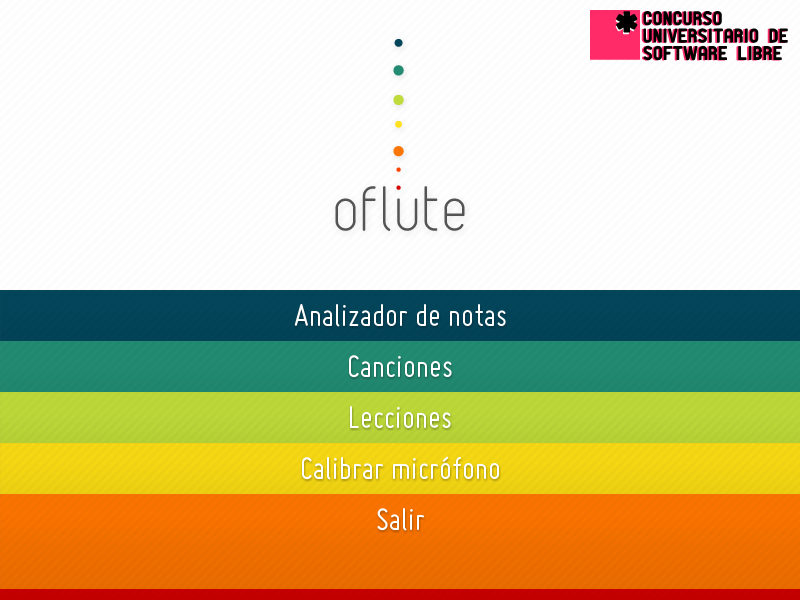
\includegraphics[width=0.8\textwidth]{imagen_menuPrincipal}
  \caption{Pantalla del menú principal}
\end{figure}

\pagebreak

\begin{figure}[htp!]
  \centering
  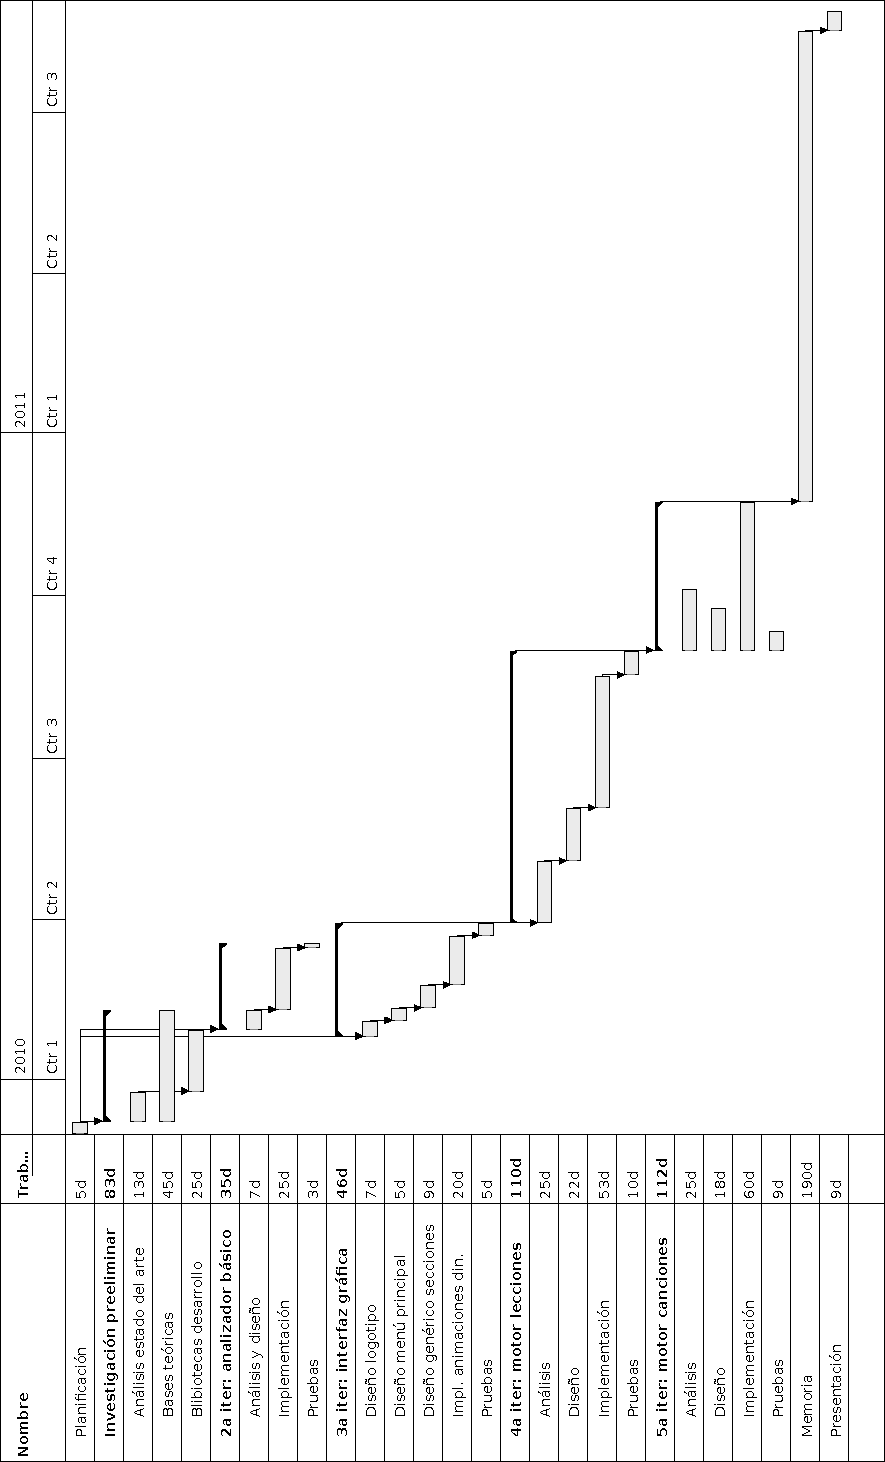
\includegraphics[width=0.95\textwidth]{imagen_diagrama_gantt}
  \caption{Diagrama Gantt de iteraciones}
  \label{fig:gantt}
\end{figure}

\pagebreak

\subsection{Análisis de notas}
Permite a los usuarios comprobar, de manera individual y pausada, que la
interpretación de cada una de las notas en la flauta es correcta. Para ello, se
presenta un pequeño analizador que responderá al sonido emitido por el usuario
con la flauta mostrando la nota tocada en pantalla.

\begin{figure}[h!]
  \centering
  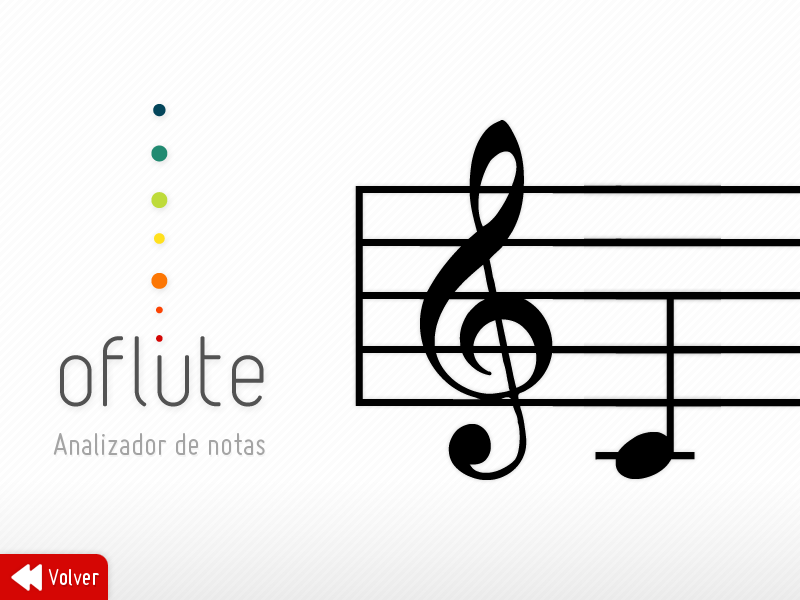
\includegraphics[width=0.8\textwidth]{imagen_seccionAnalizador}
  \caption{Pantalla del analizador de notas}
\end{figure}

\subsection{Motor de canciones}
Mediante este sistema, el usuario tendrá la oportunidad de interpretar canciones
completas a la vez que el computador analiza la eficacia del jugador,
otorgándole una puntuación en tiempo real. Además, el motor de canciones es
fácilmente expansible mediante ficheros de definición de canciones.

\subsection{Motor de lecciones}
Este sistema ofrece al usuario una serie de lecciones multimedia, con las que
podrá aprender sobre diferentes aspectos de la música en general y la flauta en
particular. Las lecciones cuentan con imágenes, texto y animaciones, que harán
que el aprendizaje sea entretenido y ameno. También es posible añadir nuevas
lecciones al sistema de forma sencilla.

\begin{figure}[h!]
  \centering
  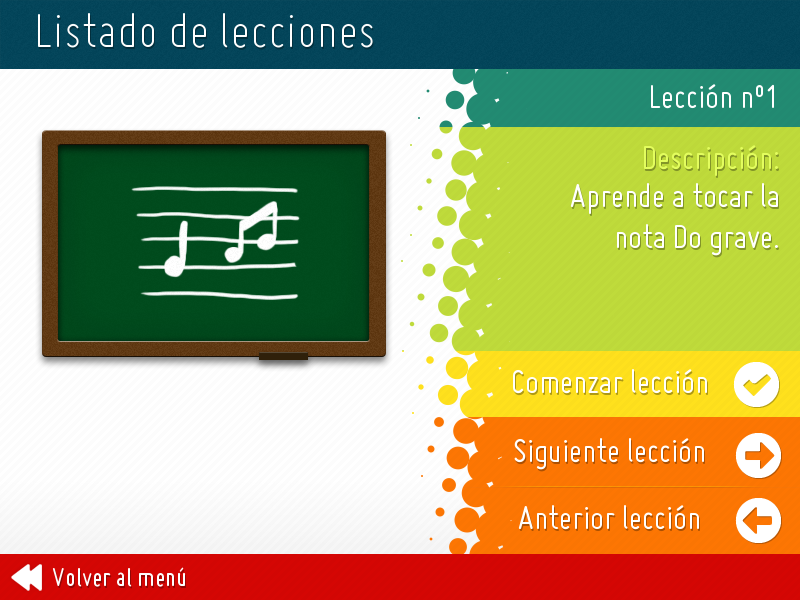
\includegraphics[width=0.8\textwidth]{imagen_seccionLecciones1}
  \caption{Pantalla del menú de selección de lecciones}
\end{figure}

\subsection{Calibración del micrófono}
\textbf{oFlute} ofrece la posibilidad de calibrar el micrófono, de forma que el
sistema se adapte al ruido ambiental y el análisis del sonido capturado sea lo
más exacto posible

\section{Implementación}
Durante el desarrollo del proyecto surgieron numerosas cuestiones y decisiones
de implementación. A continuación se presenta una selección de las que más
interés han generado. En la memoria del proyecto se desarrollan en mayor
extensión.

\subsection{Implementación del analizador básico}
La creación del analizador básico de notas era crucial para el buen transcurso
del resto del proyecto, por lo que fue uno de los objetivos que antes se
abordaron. El desarrollo se dividió en dos partes. Por un lado, había que
iniciar la captura de audio, lanzando el subsistema de sonido y empezando a
capturar datos. Por otro lado, se tenía que hacer el análisis de los datos
leídos para determinar qué nota se estaba tocando.

La gestión del subsistema de audio se hizo mediante la \textit{Simple API} de
PulseAudio, la biblioteca de audio que se empleó en oFlute. Se utilizó para la
configuración y creación de un flujo de audio de entrada que permitiera captar,
muestrear y samplear el sonido del micrófono, ofreciéndolo en forma de datos en
punto flotante en un búffer.

El siguiente paso fue el análisis del audio capturado. Para ello, utilizamos la
Transformada Rápida de Fourier mediante su implementación en la biblioteca
KissFFT. De forma iterativa, se iba analizando el búffer de sonido cada vez que
éste se llenaba, dando lugar a una aproximación de la frecuencia fundamental
capturada y, por ende, la nota que se estaba interpretando con la flauta.

Una vez implementado y probado el sistema, se dió por bueno el analizador y se
siguió construyendo el resto de la aplicación

\subsection{Carga y uso de fuentes TrueType en Gosu}
La biblioteca principal utilizada en la implementación del proyecto es Gosu, una
librería de desarrollo de videojuegos 2D, multi-plataforma y con numerosas
características. Desafortunadamente, no era posible utilizar fuentes TrueType
cuando se utilizaba la biblioteca en GNU/Linux.

Utilizando los conocimientos de otra popular biblioteca, SDL, se consiguió
implementar un sistema para cargar y usar fuentes TrueType en Gosu de forma
eficiente. Esta implementación finalmente acabó formando parte oficial de la
biblioteca Gosu.

\subsection{Animaciones dinámicas}
Una de las decisiones iniciales de diseño fue la de hacer la interfaz gráfica de
usuario lo más atractiva posible, intentando utilizar gráficos amigables y, en
la medida de lo posible, animaciones y efectos dinámicos.

Con esto, se tornaba necesario crear un sistema de animaciones lo más versátil
posible, de forma que dotar a los elementos de la interfaz de movimiento fuera
un proceso sencillo. 

Para satisfacer este objetivo se ideó una serie de clases de animación que
permiten animar las propiedades de los objetos de manera muy sencilla. Mediante
el uso de las ecuaciones de animación de Robert Penner, el sistema creado cuenta
con un gran número de opciones y diferentes formas de movimiento, según el tipo
de función utilizada para calcular los valores: cuadrático, cúbico, etcétera.

Gracias a este sistema, la interfaz de usuario de oFlute cuenta con un gran
dinamismo y vistosidad.

\subsection{Gestión de estados}
La gestión de estados es uno de los retos principales a la hora de desarrollar
un videojuego. Es necesario contar un sistema de gestión de estados robusto, que
permita pasar de un estado a otro de forma sencilla, sin errores, y manteniendo
información entre transiciones si fuera necesario.

En el caso de oFlute, se creó un gestor de estados que permitió modularizar
fácilmente el programa, haciendo una clara división entre secciones y
facilitando la transición entre ellas. Además, mediante pruebas exhaustivas y el
uso de herramientas de depuración, el gestor está implementado de forma que la
carga y descarga de estados sea limpia y sin errores, evitando fugas de memoria.

\subsection{Internacionalización}
Durante el desarrolllo del proyecto surgió la necesidad de preparar el proyecto
para su traducción. Inicialmente se optó por utilizar un sistema propio de
traducción, basado en un script en Python y en una pequeña clase que generaba un
diccionario según el idioma elegido. Sin embargo, esta opción resultó
ineficiente y, sobre todo, alejada del resto de soluciones estándar a la hora de
traducción de proyectos. 

Por ello, se decidió investigar sobre las tecnologías de traducción más
utilizadas en el panorama del software libre, y finalmente se optó por
\textbf{GNU Gettext}~\cite{refgettext}. Para afianzar los conocimientos y
facilitar el aprendizaje a otros desarrolladores, se editó un conciso manual
sobre internacionalización de proyectos, presente como apéndice en la memoria del proyecto fin de



\section{Conclusiones y difusión}
Durante el transcurso del desarrollo de oFlute, y sobre todo al término del
mismo, se han obtenido unas conclusiones y unos resultados, tanto de forma
personal como para con la comunidad, que se resumen en esta sección y se tratan
más en profundidad en el capítulo dedicado a tal efecto en la memoria principal.

\subsection{Objetivos}
Al término del desarrollo del proyecto, el proyecto ha completado todos los
objetivos a cumplir, detallados en el planteamiento inicial. En particular:

\begin{itemize}
\item Se llevó a cabo la creación del módulo de análisis de sonido, consiguiendo
  una efectividad en la detección de las notas muy alta.
\item Se hizo uso del módulo en una sección de análisis de notas y en el propio
  juego de interpretación de canciones, con resultados muy satisfactorios y
  funcionamiento correcto.
\item Además, el sistema de lecciones planteado se llevó a cabo correctamente,
  consiguiendo un motor dinámico bastante potente y fácilmente ampliable, con
  opción a añadir nuevas lecciones al sistema.
\item Finalmente, todos los objetivos se llevaron a cabo respetando la premisa
  de mantener una interfaz de usuario amigable y fluida, agradable a la vista y
  sencilla de usar.
\end{itemize}

\subsection{Posibles mejoras}
Hay un gran número de posibles mejoras y extensiones de la funcionalidad de
oFlute, en unos casos descubiertas de forma personal y en otros casos aportadas
por terceras personas. Algunas de las más interesantes son las siguientes:
\begin{itemize}
\item Extensión del sistema de lecciones para permitir lecciones de varios
  pasos, así como integrar las lecciones con el analizador de audio para
  comprobar los conocimientos in-situ.
\item Mejora de la jugabilidad del sistema de canciones, añadiendo bonus y
  puntos extra.
\item Intentar extender el sistema a otros instrumentos o a la voz humana.
\item Portar el videojuego a la plataforma Windows.
\end{itemize}

\subsection{Conclusiones personales}

oFlute ha sido el proyecto más longevo al que me he enfrentado hasta ahora. A
pesar de tener conciencia de la envergadura del mismo desde el principio, el
tiempo para completarlo ha superado todas mis expectativas, sobre todo en lo que
a documentación se refiere. 

Gracias a oFlute he aprendido las técnicas básicas de la programación de audio,
sobre todo en la parte técnica más que teórica. Es esta parte teórica, sobre
todo la de análisis, la que me gustaría reforzar en un futuro, ahora que cuento
con las bases para conseguirlo. Los videojuegos relacionados con el audio
son un nicho aún poco explorado y que puede dar muchas satisfacciones, sobre
todo cuando el producto se orienta a un público joven.

Por otro lado, oFlute también me ha ayudado a aprender a usar bastantes
tecnologías auxiliares, en algunos casos meras herramientas que han facilitado
el trabajo y, en otros casos, elementos que resultaron ser de inestimable ayuda
e imprescindible uso al término del proyecto.

Una de estas tecnologías es \textbf{Boost}~\cite{boost}, un conjunto de
bibliotecas para C++ que amplían en gran medida la biblioteca estándar del
lenguaje. Un amplio número de componentes de Boost formarán parte del nuevo
estándar C++0x, por lo que me ha servido para ponerme al día en las novedades
que están por llegar.

Al tratarse de la principal biblioteca utilizada durante el desarrollo, oFlute
me ha provisto de un profundo conocimiento de \textbf{Gosu}~\cite{gosu},
permitiéndome implementar videojuegos con mucha más fluidez y labrándome un
pequeño \textit{framework} personal que utilizar de base en próximos
proyectos. 

Otra de las tecnologías que he aprendido ha sido \textbf{GNU Gettext}, que ha
servido para internacionalizar el proyecto. Aunque inicialmente se pensó en
utilizar una solución propia para la internacionalización el proyecto,
posteriormente se decidió usar esta tecnología, ampliamente conocida y
utilizada.

\subsection{Difusión}

\subsubsection{Conocimiento generado}

Además de servir como recurso para el correcto transcurso del proyecto, los
conocimientos adquiridos me permitieron, en numerosos casos, generar
documentación adicional e impartir talleres relacionados las tecnologías
previamente mencionadas.

En cuanto a Boost, se llevó a cabo un taller durante los \textit{Cursos de
  Verano de la OSLUCA}~\cite{cursosverano}, en el que se explicaron las partes
más importantes de esta colección de bibliotecas, con numerosos ejemplos de
muchas de ellas. Toda la documentación es libre~\cite{materialesCursoBoost}.

Por otro lado, impartí un taller~\cite{tallergosu} sobre la biblioteca Gosu en
colaboración con la ADVUCA~\cite{advuca}, cuya afluencia superó las 50
personas. Los materiales pueden descargarse
libremente~\cite{tallergosumateriales}.

Por último, tras la aplicación de GNU Gettext en oFlute, escribí una guía
concisa sobre traducción de proyectos con esta herramienta, que se puede
encontrar en uno de los apéndices de la memoria, así como de forma online en la
url \url{http://hdl.handle.net/10498/10772}.


\subsubsection{Freegemas}

Uno de los proyectos \textit{``hijos''} de oFlute ha sido
\textbf{Freegemas}~\cite{freegemas}, un clon libre del popular juego tipo puzzle
\textit{Bejeweled}. Freegemas es multiplataforma, funciona tanto en GNU/Linux
como en Windows, y además forma parte oficial de Guadalinex~\cite{guadalinex},
por lo que es posible encontrarlo en los repositorios oficiales.

Además, Freegemas sirvió como base para una serie de tres artículos que
publiqué, junto al director del presente PFC, en la revista Linux
Magazine~\cite{linuxmagazine} sobre desarrollo de videojuegos en C++. Es posible
encontrar estos artículos en el archivo de la
revista~\cite{refarticulo1}~\cite{refarticulo2}~\cite{refarticulo3} bajo una
licencia Creative Commons.

\subsubsection{IV Concurso Universitario de Software Libre}

Por otro lado, gracias a oFlute tuve la oportunidad de participar en el IV
Concurso Universitario de Software Libre~\cite{cusl}. En el transcurso del
concurso formé parte de una comunidad muy unida, en la que reinó el apoyo y la
ayuda entre los concursantes. La final del concurso se celebró en la Escuela
Superior de Ingeniería de Cádiz, en la que oFlute obtuvo una mención
especial~\cite{cusl2}.

Previa a la final nacional tuvo lugar la fase local del concurso, en el que el
proyecto también recibió un accésit al mejor proyecto de
innovación~\cite{cusllocal}.

\bibliographystyle{hispa-annote}
\bibliography{bibliografia}

\end{document}

 
\chapter{Conclusiones}
%\begin{frame}{Conclusiones a nivel de proyecto}
  \begin{block}{Objetivos cumplidos}
    Se completaron todos los objetivos propuestos:
    \begin{itemize}
    \item Se creó un módulo de análisis de notas eficiente.
    \item El sistema de canciones integró el módulo de análisis de forma
      efectiva.
    \item Desarrollamos un sistema de lecciones muy completo.
    \item Se mantuvo en todo momento una interfaz agradable y fluida.
    \end{itemize}    
  \end{block} 
\end{frame}

\begin{frame}{Conclusiones a nivel de proyecto}
  \begin{block}{Posibles mejoras}
    Hay lugar para ampliar el proyecto:
    \begin{itemize}
    \item Extender el sistema de lecciones para añadir, por ejemplo, vídeos y
      otros elementos multimedia.
    \item Mejorar la jugabilidad del sistema de canciones.
    \item Portar el juego a otras plataformas.
    \end{itemize}
  \end{block}  
\end{frame}

\begin{frame}{Conclusiones a nivel personal}
  \begin{itemize}
  \item Proyecto muy longevo.
  \item Mucho conocimiento nuevo adquirido: DSP, programación de audio, hilos,
    matemáticas...
  \item Mucho conocimiento generado.
  \item Cercano a proyectos comerciales.
  \end{itemize}
\end{frame}

\begin{frame}{Conocimiento generado}
  \pause

  \begin{block}{Taller de Boost}
    Se explicaron las partes más importantes de esta colección de bibliotecas,
    con numerosos ejemplos.
  \end{block}

  \pause

  \begin{block}{Taller de Gosu}
    Más de 50 asistentes, desarrollo de un clon del Arkanoid.
  \end{block}

  \pause

  \begin{block}{Tutorial de Gettext}
    Completo manual de internacionalización de proyectos. También se hizo un
    taller sobre el mismo tema.
  \end{block}
\end{frame}

\begin{frame}{Proyectos derivados}

  \begin{center}
    A partir del código de oFlute se desarrolló \textbf{Freegemas}, clon
    libre y multiplataforma de Bejeweled.

    \medskip

    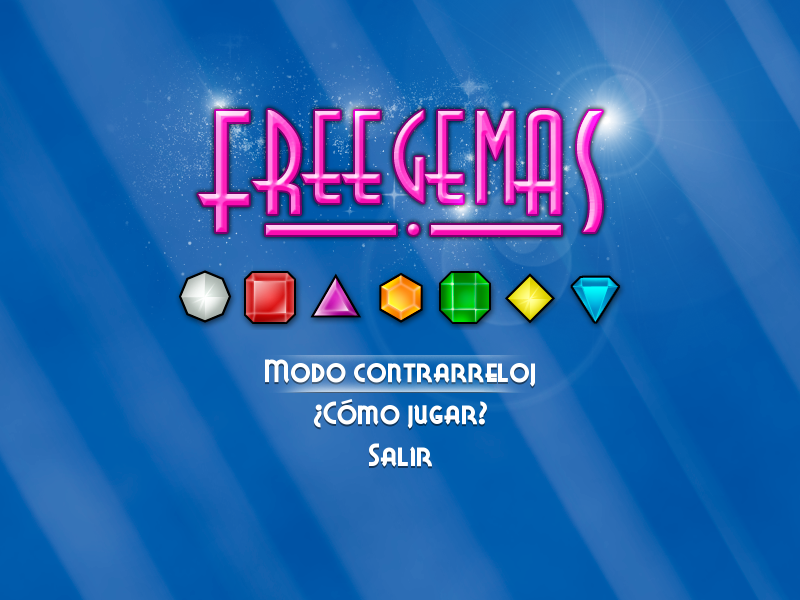
\includegraphics[width=0.49\textwidth]{imagenes/imagen_freegemas1}\hspace{0.1cm}
    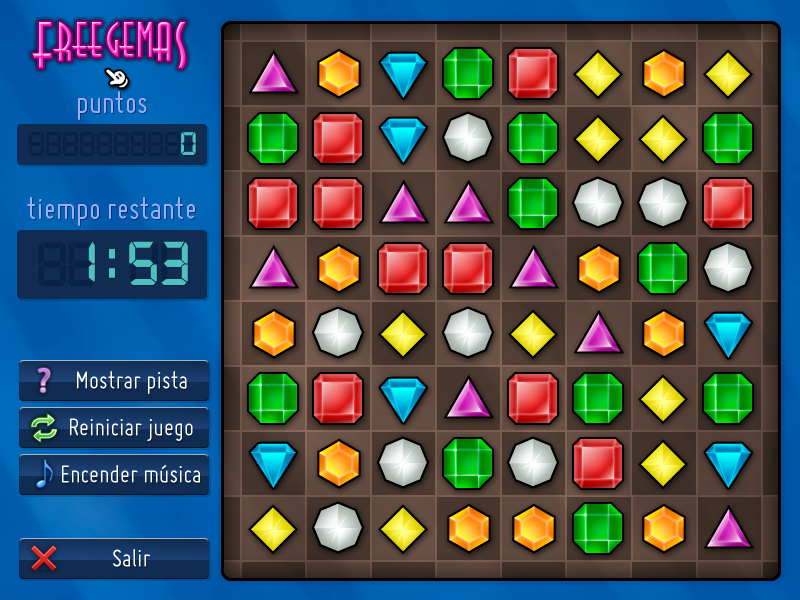
\includegraphics[width=0.49\textwidth]{imagenes/imagen_freegemas2}

    \medskip

    \begin{itemize}
    \item \textbf{Tres publicaciones} en Linux Magazine.
    \item \textbf{Inclusión oficial} en Guadalinex v8.
    \end{itemize}
  \end{center}
\end{frame}

\begin{frame}{Difusión}
  \begin{block}{Social media}
    \begin{itemize}
    \item Blog: \url{oflute.wordpress.com}, 5500 visitas en total.
    \item 3 vídeos en YouTube, aprox. 700 reproducciones.
    \end{itemize}    
  \end{block}

  \pause

  \begin{block}{Forja}
    \begin{itemize}
    \item \url{http://oflute.googlecode.com}
    \item Más de 270 revisiones.
    \item Aprox. 8000 líneas de código.
    \end{itemize}
  \end{block}

  \pause

  \begin{block}{Referencia del código}
    \begin{itemize}
    \item Generada con \textbf{Doxygen}.
    \item Disponible en la forja.
    \item Accesible en \url{http://www.josetomastocino.com/oflute}.
    \end{itemize}
  \end{block}
\end{frame}

\begin{frame}{Difusión}
  \begin{block}{Concurso Universitario de Software Libre}
    \begin{itemize}
    \item Mención especial a nivel nacional.
    \item Accésit al mejor proyecto de innovación en la fase local.
    \end{itemize}
  \end{block}
  
  \pause

  \begin{block}{Guadalinex}
    \begin{itemize}
    \item oFlute se encuentra  en los repositorios de \textbf{Guadalinex}.
    \end{itemize}
  \end{block}
\end{frame}
%%% Local Variables: 
%%% mode: latex
%%% TeX-master: "../presentacion"
%%% End: 


\chapter{Manual del usuario}
%%
% Generado autom�ticamente por las hojas de estilo XSLT
% Modificado posteriormente a mano
%
% Antonio Garc�a Dom�nguez, (C) 2008
% nyoescape@gmail.com
% $Id$
%

\section{Instalaci�n de XMLEye}
\label{instPrograma}

 En este apartado cubrir� la instalaci�n de XMLEye en sus diferentes formas, tanto a nivel de usuario local como a nivel de sistema. Para instalar los conversores asociados y sus hojas de usuario y descriptores de formato, referirse al apartado~\ref{instHojas} (p�gina~\pageref{instHojas}). 

\subsection{Requisitos previos}

 Se necesita tener instalado un entorno Java compatible con J2SE 5.0 o superior. Su instalaci�n se realiza autom�ticamente si utilizamos los paquetes Debian. 

\subsubsection{Windows}

 Tendremos que ir a \url{http://java.sun.com/javase/downloads/index.jsp} y descargar una edici�n reciente del JRE de acuerdo a nuestro sistema operativo. Tanto si hemos obtenido la versi�n que no requiere conexi�n como la que descarga s�lo lo necesario a trav�s de Internet, todo lo que tendremos que hacer es ejecutar el instalador y seguir las instrucciones. 

\subsubsection{GNU/Linux}

 Si utilizamos una distribuci�n basada en Debian, podemos probar a instalar los paquetes \filename{icedtea\hyp{}7\hyp{}jre} o \filename{openjdk\hyp{}6\hyp{}jre}. OpenJDK es la iniciativa de Sun, que a fecha de hoy (03/07/2008) es pr�cticamente 100 \% libre salvo por algunas peque�as partes que el proyecto IcedTea ha reemplazado utilizando c�digo del proyecto GNU Classpath. Podemos instalar una versi�n de OpenJDK 6.0 con los reemplazos de IcedTea en Ubuntu 8.04 "Hardy Heron" y usarla como entorno Java por defecto con estas �rdenes: 

\begin{alltt}
	\command{sudo aptitude install openjdk-6-jre}
	\command{sudo update-alternatives --config java}
\end{alltt}

 Escogeremos la entrada de \filename{openjdk\hyp{}6\hyp{}jre} y pulsaremos Intro, terminando con este paso. Si estamos utilizando openSUSE 10.3, podemos usar sin problemas el entorno J2SE 5.0 de Sun que incluye de f�brica. En caso de que no estuviera instalado por alguna raz�n, tendr�amos que instalar los paquetes \filename{java\hyp{}1\_5\_0\hyp{}sun*} a trav�s del gestor de paquetes de YaST. 

\note{ Actualmente, OpenJDK sigue teniendo peque�os defectos en la forma en que sit�a los componentes Swing. Es posible que algunos di�logos tengan un aspecto distinto al normal, con botones demasiado grandes, por ejemplo. El JRE original de Sun no tiene estos problemas, pero no es 100 \% libre. De todas formas, los efectos de este problema son puramente est�ticos. }

\subsection{Instalaci�n desde distribuciones precompiladas}

\note{ Si se usa una distribuci�n basada en Debian, se deber�a considerar el uso de los paquetes Debian, que son mucho m�s c�modos de usar. }

\subsubsection{Un �nico usuario, GNU/Linux}

 El proceso es muy sencillo: s�lo hay que descargar el \filename{\hyp{}dist\hyp{}tar.gz} m�s reciente de XMLEye de \url{https://forja.rediris.es/frs/?group_id=233} y descomprimirlo bajo nuestro directorio personal. Para ejecutar XMLEye, basta con ejecutar el gui�n \filename{/home/\-\emph{usuario}/\-xmleye/\-xmleye} tras pulsar la combinaci�n \keycombo{ALT + F2}. Una opci�n m�s c�moda para los habituales de la l�nea de �rdenes es a�adir la siguiente l�nea a \filename{\~\{\}/\-.bashrc}: 

\begin{alltt}
export PATH=\$PATH:\~{}/xmleye
\end{alltt}

 Haciendo esto, se puede abrir cualquier documento compatible desde la l�nea de �rdenes mediante: 

\begin{alltt}
xmleye \emph{(ruta absoluta o relativa)}
\end{alltt}

 Seg�n este procedimiento, las hojas de usuario se instalar�n en \filename{/home/\-\emph{usuario}/\-xmleye/\-xslt}, y los descriptores de formatos en \filename{/home/\-\emph{usuario}/\-xmleye/\-formats}. Las opciones se guardar�n en \filename{/home/\-\emph{usuario}/\-xmleye}. 

\subsubsection{M�ltiples usuarios, GNU/Linux}

 Un caso m�s complejo es cuando queremos instalarlo para varios usuarios, pero queremos tener ajustes distintos para cada usuario (las hojas son comunes a todos). Al igual que en el caso anterior, deberemos tener instalado un JRE compatible con J2SE 5.0 o superior antes que nada, pero despu�s usaremos una distribuci�n diferente de los ficheros. 

 La distribuci�n "ideal" ser�a la del paquete Debian, pero como es un poco m�s compleja de lo que necesitamos, nos limitaremos a un t�rmino medio. Primero descomprimiremos la �ltima distribuci�n de XMLEye (el enlace de descarga est� en la secci�n anterior) a \filename{/opt}, que crearemos si no existe ya: 

\begin{alltt}
sudo mkdir /opt
cd /opt
sudo tar xjf \emph{(ruta a distribuci�n)}

\end{alltt}

 Tendremos que retocar el gui�n de lanzamiento un poco. XMLEye cuenta con dos variables de entorno, \envar{XMLEYE\_PREF\_DIR} y \envar{XMLEYE\_FORMATS\_DIR}, que indican la ruta en la que se guardar�n las preferencias y los formatos personalizados por el usuario. Adem�s, XMLEye supone que las hojas de usuario se hallan bajo el subdirectorio \filename{xslt} de la ruta sobre la cual es lanzado. 

 Teniendo todo esto en cuenta, habr� que sustituir las l�neas que afectan a \envar{PROGRAM\_DIR} y \envar{PROGRAM\_JAR} por: 

\begin{alltt}
PROGRAM\_DIR=/opt/xmleye
PROGRAM\_JAR=xmleye.jar
export XMLEYE\_PREF\_DIR=\${HOME}/.xmleye
export XMLEYE\_FORMATS\_DIR=\${HOME}/.xmleye
mkdir -p \${XMLEYE\_PREF\_DIR}
\end{alltt}

 De forma similar a la secci�n anterior, los usuarios podr�an directamente ejecutar XMLEye a trav�s de la ruta completa. Para que todos los usuarios puedan ejecutar XMLEye por nombre, se puede a�adir esta l�nea a \filename{/etc/\-environment}: 

\begin{alltt}
export PATH=\$PATH:/opt/xmleye
\end{alltt}

 Si queremos que aparezca una entrada de men� y que se asocien los ficheros XML con XMLEye, entonces tendremos que, adem�s de seguir el paso anterior, crear el fichero \filename{/usr/\-share/\-applications/\-xmleye.desktop} con este contenido: 

\begin{alltt}
[Desktop Entry]
Encoding=UTF-8
Version=1.0
Type=Application
Terminal=false
Exec=xmleye  \%U
Comment[es]=Visor gen�rico de XML dirigido por datos
Name=XMLEye
Comment=Generic data-driven XML Viewer
GenericName=Generic XML viewer
GenericName[es]=Visor gen�rico de XML
Icon=accessories-text-editor
Categories=Utility;TextEditor;
MimeType=application/xml;
\end{alltt}

 Actualizaremos las bases de datos y reiniciaremos los men�s de GNOME con: 

\begin{alltt}
sudo update-desktop-database
sudo update-menus
sudo killall gnome-panel nautilus
\end{alltt}

 Ya deber�a de aparecer la entrada de XMLEye en el men� principal de GNOME. 

 Las hojas de usuario estar�n bajo \filename{/opt/\-xmleye/\-xslt}, y los descriptores de formato en \filename{/opt/\-xmleye/\-formats}. 

\subsubsection{Windows}

 Descargamos y descomprimimos en alguna carpeta el \filename{\hyp{}dist\hyp{}tar.gz} m�s reciente de XMLEye de \url{https://forja.rediris.es/frs/?group_id=233}. 

 Para ejecutar XMLEye, haremos doble clic en el fichero \filename{xmleye.jar} de la carpeta en que hemos descomprimido la distribuci�n. 

\subsection{Instalaci�n desde paquetes Debian}

 Esta es la opci�n a seguir siempre que sea posible, ya que adem�s de ser m�s sencilla, permitir� recibir actualizaciones de forma autom�tica. 

 Los paquetes han sido desarrollados para Ubuntu Gutsy, pero deber�an funcionar en cualquier distribuci�n basada en Debian reciente. 

 Los pasos a seguir son: 

\begin{enumerate}
\item Descargaremos la firma digital de los paquetes disponible bajo \url{http://www.shoyusauce.org/packages/claveDebian.asc}.

\item  A�adiremos la firma al anillo de confianza de Apt. En primer lugar lanzaremos la opci�n \emph{Sistema $\rightarrow$ Administraci�n $\rightarrow$ Or�genes
	  de software} bajo el men� principal de GNOME. 

 Hecho esto, seleccionaremos la pesta�a \guilabel[moreinfo = none]{Autentificaci�n} y pulsaremos en el bot�n \guibutton[moreinfo = none]{Importar clave...}, tras lo cual seleccionaremos la firma que antes descargamos. 

 A�n no cerraremos la ventana: nos queda una cosa por hacer. 

\item  Ahora a�adiremos los repositorios de paquetes binarios y paquetes de fuentes de \application{XMLEye} y sus hojas de estilos. Esta vez iremos a la pesta�a \guilabel[moreinfo = none]{Software de terceros}. 

 Pulsaremos en \guibutton[moreinfo = none]{A�adir} e introduciremos esta l�nea tal y como est�: 

\begin{alltt}
deb http://www.shoyusauce.org/packages/ubuntu/ gutsy main
\end{alltt}

 Volvemos a pulsar en \guibutton[moreinfo = none]{A�adir}, pero esta vez introducimos esta l�nea: 

\begin{alltt}
deb-src http://www.shoyusauce.org/packages/ubuntu/ gutsy main
\end{alltt}

 Ya podemos pulsar en \guibutton[moreinfo = none]{Cerrar} para cerrar este di�logo, y solicitar la actualizaci�n de nuestras listas de paquetes en el di�logo subsecuente pulsando en \guibutton[moreinfo = none]{Recargar}. Una vez haya terminado, estaremos listos para instalar \application{XMLEye} y otros paquetes de apoyo, como \application{pprocACL2}. 

\item  Lanzaremos \emph{Sistema $\rightarrow$ Administraci�n $\rightarrow$ Gestor
	  de paquetes Synaptic} y pulsaremos en el bot�n \guibutton[moreinfo = none]{Buscar} de la barra de herramientas. 

 Introduciendo "xmleye" en el campo de b�squeda obtendremos un �nico resultado en el que podremos hacer doble clic para marcar para su instalaci�n. Tambi�n podr�amos seleccionar otros paquetes con los conversores, descriptores y hojas de estilos espec�ficas de otros formatos, como "libacl2-procesador-perl" o "libyaxml-reverse-perl", de la misma forma. 

 Una vez todos los paquetes que deseamos instalar se hallen marcados, pulsaremos en \guibutton[moreinfo = none]{Aplicar} de la barra de herramientas para confirmar los cambios. 

\item  �Listo! Ya podemos lanzar XMLEye a trav�s de \emph{Aplicaciones $\rightarrow$ Accesorios $\rightarrow$ XMLEye} del men� principal de GNOME. 

\note{ S�lo un detalle: todas las opciones que establezcamos ir�n a parar al subdirectorio \filename{.xmleye} bajo nuestro directorio personal, es decir, \filename{/home/\-\emph{nombredeusuario}}. }

\end{enumerate}

 La ruta bajo la cual tendremos que instalar las hojas de usuario ser� \filename{/usr/\-share/\-xmleye/\-xslt}, y en \filename{/usr/\-share/\-xmleye/\-formats} se hallar�n los descriptores de formato. 

\subsection{Compilaci�n del c�digo fuente}

\note{ Aunque hay instant�neas disponibles del c�digo fuente, �stas son m�s para los usuarios que los desarrolladores. En caso de querer participar como desarrollador, recomiendo encarecidamente usar una copia de trabajo del repositorio Subversion. Bastar� con instalar el paquete \filename{subversion} y seguir algunas instrucciones sencillas. Para m�s informaci�n, v�ase el excelente libro~\cite{svnhandbook}. }

 Tras obtener un JDK compatible con J2SE 5.0 o superior, como el de OpenJDK 6.0 o 7.0, IcedTea 6.0 o 7.0, o los originales de Sun, tendremos que instalar adem�s la herramienta Apache Ant y el entorno de pruebas de unidad JUnit, en una de sus versiones 3.X. En Ubuntu 8.04 "Hardy Heron", esto se puede hacer mediante: 

\begin{alltt}
sudo aptitude install openjdk-6-jdk ant junit
\end{alltt}

 Ahora tendremos que crear una copia de trabajo local de la �ltima revisi�n de la rama principal de desarrollo del repositorio de RedIris: 

\begin{verbatim}
svn checkout \
  https://forja.rediris.es/svn/csl2-xmleye/XMLEye/trunk \
  xmleye
\end{verbatim}

 Ya podemos introducirnos en \filename{xmleye} y aprovechar los objetivos ya definidos en el fichero \filename{build.xml} de Ant. Si se desea instalar \filename{xmleye} a partir de fuentes, se recomienda usar el objetivo \varname{dist} e instalar la distribuci�n seg�n alguno de los m�todos antes expuestos. 

\begin{description}
\item[clean] \mbox{}
Limpia el �rbol de directorios existente.

\item[compile] \mbox{}
Compila todo el c�digo fuente.

\item[dist] \mbox{}
Compila las fuentes ,ejecuta las pruebas de unidad y genera una distribuci�n autocontenida en el subdirectorio \filename{dist}.

\item[dist-jar] \mbox{}
Tras compilar y ejecutar las pruebas de unidad, genera un fichero \filename{.jar} bajo \filename{dist}, pero no llega a empaquetarlo con todo lo dem�s.

\item[docs] \mbox{}
Genera la documentaci�n del API en formato HTML en el subdirectorio \filename{docs} a trav�s de Javadoc.

\item[run] \mbox{}
Se trata del objetivo por defecto (ejecutado a trav�s de \command{ant}). Compila el c�digo y ejecuta la versi�n as� compilada de XMLEye.

\item[run-about] \mbox{}
Compila el c�digo y ejecuta �nicamente la ventana de "Acerca de". �til a la hora de dise�ar la interfaz.

\item[run-find] \mbox{}
Como la anterior, pero para el di�logo de b�squeda.

\item[run-types] \mbox{}
M�s de lo mismo, pero para el di�logo de edici�n de tipos.

\item[test] \mbox{}
Ejecuta las pruebas de unidad. La salida de cada conjunto de pruebas se halla bajo el fichero \filename{TEST\hyp{}*} correspondiente.

\end{description}

 M�s cosas a tener en cuenta: esta aplicaci�n depende de InfoNode Tabbed Panel 1.5.0 (licenciado bajo la GPL para uso no comercial) y del look and feel JGoodies Looks 2.1.4 (licenciado bajo BSD), disponibles en \url{http://www.infonode.net/index.html?itp} y \url{https://looks.dev.java.net/} respectivamente. De todas formas, los ficheros \filename{.jar} necesarios se hallan en el propio repositorio, por lo que no hay que hacer nada al respecto. 

 Adem�s, el desarrollo puede hacerse mucho m�s c�modamente si se emplea el plugin Subclipse para Eclipse, disponible en \url{http://subclipse.tigris.org/}, y se importa a trav�s de �l el proyecto Eclipse desde el repositorio. As� podemos contar con sus funcionalidades de refactorizaci�n y notificaci�n de errores y avisos de compilaci�n en directo. 

\section{Instalaci�n de conversores asociados}

\label{instHojas}

\subsection{\nombrepostprocesador{}: convertidor de demostraciones de ACL2}

 Como muestra de las capacidades de XMLEye, desarroll� en paralelo un conjunto de hojas de usuario de preprocesado y visualizaci�n, junto con un tipo de documento para ACL2. Esto nos permite demostraciones para dicho sistema en formato \filename{.lisp} siguiendo una estructura arb�rea donde cada nodo se muestra como un hipertexto con enlaces a otras partes de la demostraci�n. 

 La subcarpeta \filename{t/\-testInputs} del fichero de fuentes con nombre de la forma \filename{ACL2\hyp{}Procesador\hyp{}*.tar.gz} m�s reciente contiene algunos ejemplos de inter�s, extra�dos de tutoriales reales de aprendizaje del uso de ACL2. 

 Primero nos ocuparemos de las dependencias, y luego veremos tres formas de instalar el convertidor, el descriptor de formato y las hojas de usuario. 

\subsubsection{Dependencias}

Las dependencias a instalar variar�n seg�n el m�todo de instalaci�n.

\paragraph{ACL2 2.9 o superior}

 Se ha depurado \postprocesador{} tambi�n con ACL2 3.1 y 3.3. 

\subparagraph{GNU/Linux}

En una distribuci�n basada en Debian, instalar ACL2 es tan sencillo como ejecutar la siguiente orden (necesitamos \application{gcc} para poder certificar libros):

\begin{alltt}
\command{sudo aptitude install acl2 gcc}
\end{alltt}

Otras distribuciones requerir�n del proceso manual de instalaci�n, documentado bajo \url{http://www.cs.utexas.edu/users/moore/acl2/v3-3/installation/installation.html}. Es sencillo, pero la compilaci�n de los libros puede llevar mucho tiempo (alrededor de 8-10 horas).

\subparagraph{Windows}

Descargaremos e instalaremos la distribuci�n completa de ACL2 preparada por Jared Davis, disponible en \url{http://www.cs.utexas.edu/users/moore/acl2/v3-3/distrib/windows/}. Incluye todo lo que podr�amos necesitar para trabajar con ACL2:

\begin{itemize}
\item ACL2 3.3

\item GCL 2.6.7, el entorno Lisp que necesitamos, junto con el compilador GCC necesario para certificar libros.

\item El editor GNU Emacs en su versi�n 21.3.

\item Documentaci�n de ACL2.

\item Una colecci�n de libros previamente certificados.

\end{itemize}

\paragraph{Perl 5.8.6 o superior}
\label{inst_perl}
\subparagraph{GNU/Linux}

 La gran mayor�a de las distribuciones lo incluyen de f�brica, pero en el caso en que no lo tuvi�ramos, podr�amos instalarlo en una distribuci�n basada en Debian con: 

\begin{alltt}
\command{sudo aptitude install perl}
\end{alltt}

Otra opci�n ser�a descargar el c�digo fuente de \url{http://www.perl.com/download.csp} y compilarlo, pero no se cubrir� dicha alternativa aqu�.

\subparagraph{Windows}

 Utilizaremos la edici�n 5.10 m�s reciente de Strawberry Perl, disponible bajo \url{http://strawberryperl.com/}. S�lo hemos de seguir los pasos del instalador. 

\paragraph{M�dulos Perl: \application{PAR}}
\label{inst_par}
 Una vez hayamos instalado Perl (v�ase la secci�n ), s�lo necesitamos ejecutar una orden m�s. No es necesario seguir la configuraci�n manual del acceso a CPAN en ninguno de los dos casos. 

\subparagraph{GNU/Linux}

\begin{alltt}
\command{sudo cpan PAR}
\end{alltt}

\subparagraph{Windows}

\begin{alltt}
\command{cpan PAR}
\end{alltt}

\paragraph{M�dulos Perl: \application{PAR::Packer}}
\label{inst_parpacker}
\subparagraph{GNU/Linux}

 Si estamos usando una distribuci�n basada en Debian reciente, podemos ejecutar: 

\begin{alltt}
\command{sudo aptitude install libpar-packer-perl}
\end{alltt}

 De lo contrario, ejecutaremos: 

\begin{alltt}
\command{sudo cpan PAR::Packer}
\end{alltt}

\subparagraph{Windows}

 Tendremos que obtener la �ltima copia del c�digo fuente de \application{PAR::Packer} del repositorio SVN, ya que la versi�n m�s reciente en el CPAN a d�a de hoy (03/07/2008), la 0.980, no incluye el arreglo de un defecto que imposibilitaba su instalaci�n en Strawberry Perl. Para ello, instalaremos el cliente Subversion TortoiseSVN, disponible bajo \url{http://tortoisesvn.tigris.org/}, y haremos un \emph{checkout} de la direcci�n \url{http://svn.openfoundry.org/par/PAR-Packer/trunk/}. 

 Una vez hayamos descargado el c�digo, abriremos una ventana del int�rprete de �rdenes, y dentro del directorio con el c�digo fuente, ejecutaremos: 

\begin{alltt}
\computeroutput{perl Makefile.PL
dmake
dmake test
dmake install
}
\end{alltt}

 Si se nos pide instalar alguna dependencia en alguno de los pasos, aceptaremos. 

\paragraph{Biblioteca \application{libxml2}}
\label{inst_xml}
\subparagraph{GNU/Linux}

 Si estamos usando una distribuci�n basada en Debian, ejecutaremos esta orden: 

\begin{alltt}
\command{sudo aptitude install libxml2-dev}
\end{alltt}

\subparagraph{Windows}

 No hay que hacer nada: viene ya incluida con Strawberry Perl. 

\subsubsection{Instalaci�n mediante paquetes Debian}

 Si instalamos XMLEye mediante el paquete Debian, s�lo tendremos que instalar el paquete \filename{libacl2\hyp{}procesador\hyp{}perl}. La pr�xima vez que iniciemos XMLEye tendremos todo lo necesario a nuestra disposici�n, incluido ACL2. 

\subsubsection{Instalaci�n desde distribuci�n monol�tica}
\label{inst_distrib_monolit}
 Necesitaremos previamente haber instalado ACL2, y haber instalado XMLEye descomprimiendo la distribuci�n de la forja. Descargaremos del �rea de ficheros (\url{http://forja.rediris.es/frs/?group_id=233}) de la forja de XMLEye el fichero \filename{ACL2\hyp{}Procesador\hyp{}*\hyp{}standalone\hyp{}*.tar.gz} m�s reciente que se corresponda con la microarquitectura de nuestra CPU y nuestro sistema operativo, y lo descomprimiremos sobre el directorio en el que instalamos XMLEye. 

\subsubsection{Instalaci�n desde distribuci�n basada en PAR}
\label{inst_distrib_par}
 Necesitaremos ACL2, Perl y el m�dulo PAR. El proceso es id�ntico al de~\ref{inst_distrib_monolit} (p�gina~\pageref{inst_distrib_monolit}), pero en este caso el fichero a descargar y descomprimir es \filename{ACL2\hyp{}Procesador\hyp{}*\hyp{}par\hyp{}noarch.tar.gz}, que es independiente de la CPU y el sistema operativo escogido. 

\subsubsection{Instalaci�n manual a partir de fuentes}
\label{inst_fuentes}
 Los pasos, tras instalar todas las dependencias, son los siguientes: 

\begin{enumerate}
\item Descomprimimos el fichero de fuentes bajo \filename{/tmp}, y nos introducimos en sus contenidos:

\begin{alltt}
cd /tmp
tar xzf \emph{(ruta a las fuentes)}
cd ACL2-Procesador-*
\end{alltt}

\item Instalamos el preprocesador tal y como instalar�amos cualquier paquete Perl. Este proceso resultar� muy familiar a cualquier usuario de las \application{autotools}:

\begin{alltt}
perl Makefile.PL
sudo make
make test
sudo make install
\end{alltt}

 Es muy probable que Perl nos solicite en la primera orden instalar algunas dependencias. Siempre le diremos que s�. La �ltima orden se podr�a sustituir por \command{sudo checkinstall} si deseamos poder desinstalarlo f�cilmente, instalando \postprocesador{} como un paquete Debian. 

\item  Lo siguiente es instalar las hojas de usuario, que es tan f�cil (suponiendo que la ruta de hojas de usuario es \filename{/home/\-\emph{tunombredeuaurio}/\-xmleye/\-xslt} como: 

\begin{alltt}
cp -r xslt/* \$HOME/xmleye/xslt
\end{alltt}

\item  Terminaremos instalando el descriptor de tipo a su sitio: 

\begin{alltt}
cp types/* \$HOME/xmleye/types
\end{alltt}

\end{enumerate}

\subsubsection{Ejecuci�n independiente de XMLEye}
\label{ejecucion}
 Podemos comproabr que todo va bien ejecutando el gui�n principal. La forma de hacerlo variar� seg�n el m�todo de instalaci�n usado: 

\begin{itemize}
\item Desde el paquete Debian, o desde fuentes: \command{pprocACL2} desde cualquier ruta.

\item Desde la distribuci�n monol�tica: \command{\emph{(ruta)}/\-pprocACL2}, utilizando la ruta bajo la cual se halla instalado XMLEye. Podr�amos a�adir esta ruta al PATH si quisi�ramos.

\item Desde la distribuci�n basada en PAR: \command{perl -MPAR (ruta)/\-pprocACL2.par}, utilizando la ruta bajo la cual se halla instalado XMLEye.

\end{itemize}

 Deber�amos obtener una salida como la que viene a continuaci�n. Por razones t�cnicas, es posible que en ciertos entornos la distribuci�n basada en PAR no produzca ninguna salida, pero esto no es un problema: seguir� funcionando de forma normal una vez le pasemos un fichero de entrada, imprimi�ndose el XML resultante por salida est�ndar, y los mensajes de estado por la salida de errores. 

\begin{alltt}
\computeroutput{Usage:
  pprocACL2 [opciones] [entrada Lisp ACL2]

Options:
  --help, -h, -?
          Se limita a mostrar un mensaje corto de ayuda.

  --man, -m
          Muestra un mensaje detallado de ayuda en formato man.}
\end{alltt}

\subsection{\nombreyaxml{}: conversor de documentos YAML a XML}

 Este otro conversor se desarroll� para abrir con XMLEye la familia completa de documentos con lenguajes basados en YAML 1.1 o JSON. Al igual que \postprocesador{}, incorpora las hojas de usuario y descriptores de formatos necesarios para su funcionamiento. Incluye soporte para anclias y alias de YAML. 

 Tambi�n en este caso se pueden ver algunos ejemplos de entradas aceptadas en \filename{t/\-testInputs} de las fuentes, disponibles como ficheros con nombres del estilo de \filename{YAXML\hyp{}Reverse\hyp{}*.tar.gz} en el �rea de ficheros de la forja (\url{http://forja.rediris.es/frs/?group_id=233}). 

 Para evitar repeticiones innecesarias, aprovecharemos las instrucciones de instalaci�n de algunas de las dependencias y algunos de los pasos de los m�todos de instalaci�n de \postprocesador{}. Comentaremos �nicamente los aspectos que cambian. 

\subsubsection{Dependencias}

Hay algunas dependencias de \application{YAXML::Reverse} cuyos m�todos
de instalaci�n ya se han mencionado en la secci�n \S\ref{inst_perl}
an�loga de \postprocesador{}:

\begin{description}
\item[Perl] \mbox{}
V�ase la p�gina~\pageref{inst_perl}.

\item[PAR] \mbox{}
V�ase la p�gina~\pageref{inst_par}.

\item[PAR::Packer] \mbox{}
V�ase la p�gina~\pageref{inst_parpacker}.

\item[Bibliotecas XML] \mbox{}
V�ase la p�gina~\pageref{inst_xml}.

\end{description}

\paragraph{Bibliotecas XSLT}

 Tambi�n puede que nos hagan falta las bibliotecas para XSLT. Dependiendo del sistema operativo sobre el que trabajemos, los m�todos de instalaci�n cambiar�n. 

\subparagraph{GNU/Linux}

 Necesitaremos instalar los paquetes de desarrollo para las bibliotecas \application{exslt}, \application{gdbm} y \application{gcrypt}. En una distribuci�n basada en Debian, usaremos: 

\begin{alltt}
\computeroutput{sudo aptitude install libexslt-dev \textbackslash{}
                      libgdbm-dev  \textbackslash{}
                      libgcrypt-dev}
\end{alltt}

\subparagraph{Windows}

 Como instalar manualmente las bibliotecas es demasiado complejo, usaremos una distribuci�n precompilada del m�dulo \application{XML::LibXSLT}. Para ello, ejecutaremos esta orden bajo la interfaz de l�nea de �rdenes: 

\begin{alltt}
\computeroutput{ppm install XML::LibXSLT}
\end{alltt}

\subsubsection{Instalaci�n mediante paquetes Debian}

Una vez instalemos XMLEye mediante el paquete Debian, s�lo habr� que instalar el paquete \filename{libyaxml\hyp{}reverse\hyp{}perl}, cerrar y volver a abrir XMLEye y todo quedar� listo.

\subsubsection{Instalaci�n desde distribuci�n monol�tica}

 En este caso utilizaremos el fichero m�s reciente que concuerde con nuestro entorno que siga el patr�n \filename{YAXML\hyp{}Reverse\hyp{}*\hyp{}standalone\hyp{}*.tar.gz}. 

\subsubsection{Instalaci�n desde distribuci�n basada en PAR}

 Esta vez las distribuciones (que siguen el patr�n \filename{YAXML\hyp{}Reverse\hyp{}*\hyp{}par\hyp{}*.tar.gz}) ser�n espec�ficas del entorno, pero por lo dem�s es todo igual. 

\subsubsection{Instalaci�n manual a partir de fuentes}

 El patr�n del nombre de fichero cambia a \filename{YAXML\hyp{}Reverse\hyp{}*.tar.gz} m�s reciente, y no se necesita ACL2, sino las bibliotecas de XSLT. El resto de las dependencias siguen siendo necesarias.

\subsubsection{Ejecuci�n independiente de XMLEye}

 El proceso es an�logo al de la secci�n~\ref{ejecucion} (p�gina~\pageref{ejecucion}), pero esta vez el gui�n principal es \filename{yaml2xml} (y el PAR es \filename{yaml2xml.par}), y la salida que deber�amos obtener tendr�a que ser similar a �sta: 

\begin{alltt}
\prompt{\$ yaml2xml}

\computeroutput{yaml2xml, using YAXML::Reverse 0.3.4
Usage: yaml2xml [path to .yaml]}
\end{alltt}

\subsection{Instrucciones gen�ricas}

 Estas instrucciones son las m�s detalladas, y sirven para cualquier hoja de usuario disponible actualmente y en el futuro, siempre que no var�e el dise�o de XMLEye. 

\subsubsection{Instalaci�n de hojas de usuario}

 Una hoja de usuario nos permite mejorar XMLEye en una de las siguientes formas: 

\begin{itemize}
\item Ver la estructura de un documento XML de otra forma. Un ejemplo ser�a ver s�lo un resumen del documento, cambiar el orden para su preprocesamiento, o decorar los nodos del �rbol con nuevas etiquetas e iconos.

\item Ver el contenido de un nodo del documento de otra forma. Podemos hacer cualquier cosa que se nos ocurra con XHTML 1.1 y CSS (no hay soporte para Javascript), y establecer v�nculos entre nodos del �rbol y nodos de otros documentos.

\end{itemize}

 Realmente, no son m�s que conjuntos de hojas XSLT que siguen una determinada estructura para permitir su localizaci�n y su integraci�n con otras hojas, ya que una hoja de usuario puede ser una especializaci�n de otra hoja. 

 La ruta donde se guardan las hojas de usuario variar� dependiendo del m�todo de instalaci�n que hayamos seguido. Para m�s detalles, referirse al apartado~\ref{instPrograma} (p�gina~\pageref{instPrograma}). Nos encontraremos bajo dicha ruta una serie de ficheros (s�lo de inter�s para desarrolladores) y dos subdirectorios, \filename{preproc} y \filename{view}, en cuyo interior habr� un subdirectorio por hoja de usuario de preprocesado o visualizaci�n, respectivamente. 

 Instalar una hoja de usuario no es m�s entonces que asegurarnos que su subdirectorio se halle en el lugar correcto, y reiniciar XMLEye. Encontraremos entradas con los mismo nombres que los subdirectorio correspondientes en las entradas \emph{Preferencias $\rightarrow$ Preprocesamiento} y \emph{Preferencias $\rightarrow$ Visualizaci�n} de XMLEye. Por defecto tendremos instalado como m�nimo las hojas de usuario de preprocesado y visualizaci�n \filename{xml}, y la hoja de visualizaci�n \filename{xmlSource} a partir de la versi�n 1.22. 

\subsubsection{Instalaci�n de nuevos formatos de documentos}

 A pesar de su nombre, XMLEye puede visualizar documentos de cualquier formato, usando un conversor si no se trata de un documento XML originalmente, e integrarse con su editor (monitorizando el fichero en busca de cambios) siempre que se le d� la informaci�n correspondiente. Esa informaci�n viene integrada en un \emph{descriptor de formato de documento}. 

 Dichos descriptores se nombran usando la extensi�n \filename{.format} y siguen un formato XML sencillo, en cuyos detalles no entraremos aqu� (v�ase el Manual del Desarrollador). Lo �nico que nos importa es su instalaci�n, que es tan sencilla como copiar el fichero \filename{.format} correspondiente a la ruta de tipos que le corresponde seg�n el tipo de instalaci�n que hayamos realizado. 

 Una vez instalado y reiniciado XMLEye, podremos abrir cualquier documento que tenga las extensiones especificadas en el tipo de documento instalado sin m�s problemas, siempre que su editor y preprocesador (si tiene alguno) se hallen debidamente instalados y tengan �rdenes que puedan ejecutarse desde el directorio principal de XMLEye (posiblemente usando ejecutables bajo los directorios dentro de la variable de entorno \envar{PATH}). 

\section{Uso y configuraci�n}
\label{uso}
Este apartado de la gu�a trata acerca del empleo de XMLEye y de su configuraci�n. Para cuestiones relacionadas con la instalaci�n o con detalles de implementaci�n, referirse a los apartados anteriores o al Manual del Desarrollador, respectivamente.

A lo largo de esta gu�a nos referiremos exclusivamente a las opciones de los men�s, pero pr�cticamente toda acci�n tiene una combinaci�n equivalente en el teclado,indicada en la parte derecha del elemento del men� correspondiente (y si no, es un fallo del que se agradecer�a una notificaci�n ;-): informe de �l en \url{https://forja.rediris.es/tracker/?group_id=233} ). Adem�s, las opciones m�s comunes poseen un bot�n en la barra de herramientas, cuyo icono es una versi�n ampliada del icono de la entrada de men� correspondiente.

Podemos cambiar entre los botones de la barra de herramientas, el �rbol y el navegador mediante \keycombo{Ctrl + Tab} en de izquierda a derecha y de arriba abajo, o mediante \keycombo{Shift + Ctrl + Tab} en direcci�n inversa.\keycombo{Tab} y \keycombo{Shift + Tab} siguen funcionando tambi�n de la forma usual, pero se hallan redefinidos en el navegador para navegar por los hiperv�nculos.

La forma de lanzar el programa se detalla en la gu�a de instalaci�n, y variar� seg�n el m�todo seguido.

\subsection{Apertura y edici�n de documentos}

 Bajo el men� \guimenu[moreinfo = none]{Fichero}, disponemos de \guimenuitem[moreinfo = none]{Abrir...}, en donde podremos seleccionar un fichero de cualquier tipo, o uno de los formatos que tengamos instalados. 

 Una vez hayamos seleccionado el fichero, XMLEye detectar� a partir de la extensi�n de qu� formato se trata y aplicar� el convertidor indicado, si lo hay. Una vez el fichero se halle disponible en formato XML, pasar� por la hoja de preprocesado y se mostrar� su �rbol en pantalla junto con la visualizaci�n de su nodo ra�z. 

 Para editar el fichero fuente con el editor definido en el descriptor de formato, usaremos \guimenuitem[moreinfo = none]{Editar fuente}. Si \emph{Preferencias $\rightarrow$ Actualizaci�n
      autom�tica} se halla activo, XMLEye monitorizar� el fichero en segundo plano y actualizar� el �rbol XML cada vez que se produzcan cambios en �l, indpendientemente de si estuviera o no el editor abierto. 

 Por �ltimo, podemos acceder a los 5 �ltimos documentos abiertos con �xito, o \guimenuitem[moreinfo = none]{Salir} del programa. 

 Para cerrar un documento, actualmente no hay ninguna entrada en el men� \guimenu[moreinfo = none]{Fichero}, pero puede hacerse pulsando la cruz de su pesta�a correspondiente. Para cerrar todos los documentos, podemos pulsar en el bot�n de cierre general en el extremo derecho del componente de pesta�as. 

\subsection{Navegaci�n por los documentos}

 El documento XML tras ser preprocesado sigue una estructura arb�rea normal y corriente, por lo que podemos realizar las acciones usuales mediante las entradas del men� \guimenu[moreinfo = none]{Navegar}. En particular: 

\begin{description}
\item[Buscar...] \mbox{}
 Abre un di�logo de b�squeda en el que podemos buscar siguiendo diversos par�metros. Adem�s de las opciones usuales de b�squeda por palabras completas o por concordancia de may�sculas, se puede marcar el �mbito de la b�squeda. 

\item[Buscar siguiente] \mbox{}
 Repite la �ltima b�squeda realizada, mostrando un error en caso de que no se halla realizado una anteriormente. Si hemos llegado al �ltimo resultado de la �ltima b�squeda, volveremos al primero despu�s. 

 La repetici�n de una b�squeda es muy r�pida, ya que XMLEye se ocupa de almacenar los resultados tras la primera petici�n y va dando directamente los resultados que le siguen dispu�s. 

\item[Padre] \mbox{}
 Sube un nivel en la jerarqu�a del �rbol, o no hace nada si estamos en la ra�z. 

\item[Hijo] \mbox{}
 Baja un nivel en la jerarqu�a del �rbol, o no hace nada si estamos en un nodo hoja. 

\item[Hermano anterior] \mbox{}
 Se desplaza al anterior nodo hijo del padre del nodo actual, o no hace nada si estamos en su primer hijo. 

\item[Hermano siguiente] \mbox{}
 Se desplaza al siguiente nodo hijo del padre del nodo actual, o no hace nada si estamos en su �ltimo hijo. 

\item[Expandir todo] \mbox{}
 Expande el contenido de todos los nodos del �rbol, de tal forma que todo nodo quede directamente visible, a menos que haya sido ocultado expl�citamente por la hoja de visualizaci�n. 

\item[Contraer todo] \mbox{}
 Contrae el contenido de todos los nodos del �rbol, de tal forma que �nicamente el nodo ra�z quede visible. 

\end{description}

Aunque casi toda acci�n es accesible mediante rat�n, se recomienda
aprender los accesos directos mediante teclado, ya que agilizan
enormemente los desplazamientos. En la tabla \ref{teclado_arbol}
(p�gina~\pageref{teclado_arbol}) se listan todos los accesos directos
mediante teclado para navegar por el �rbol del documento, tras hacer
clic en �l.

\begin{table}
\centering
\begin{tabularx}{\textwidth}{| c | X |} 
\hline
Combinaci�n de teclas & \multicolumn{1}{c|}{Efecto} \\ \hline
\hline
\keycombo{Arriba} & Selecciona el nodo anterior en la vista actual del �rbol. \\ \hline
\keycombo{Abajo} & Selecciona el nodo siguiente en la vista actual del �rbol. \\ \hline
\keycombo{Izquierda} & Sube al nodo padre si el nodo est� cerrado, y cierra el nodo actual de lo contrario. \\ \hline
\keycombo{Derecha} & Abre el nodo actual si est� cerrado, y baja al primer hijo de lo contrario. \\ \hline
\keycombo{Inicio} & Selecciona el primer nodo en la vista actual del �rbol. \\ \hline
\keycombo{Fin} & Selecciona el �ltimo nodo en la vista actual del �rbol. \\ \hline
\keycombo{Alt + Arriba} & Selecciona al nodo padre del actual. \\ \hline
\keycombo{Alt + Abajo} & Selecciona al primer hijo del nodo actual. \\ \hline
\keycombo{Alt + Izquierda} & Selecciona al hermano anterior del nodo actual. \\ \hline
\keycombo{Alt + Derecha} & Selecciona al hermano siguiente del nodo actual. \\ \hline

\end{tabularx}
\caption{Accesos de teclado para navegaci�n por el �rbol}
\label{teclado_arbol}
\end{table}
 Podemos cambiar entre los documentos haciendo clic en sus pesta�as correspondientes, o pulsando en la flecha hacia abajo justo a la izquierda de la cruz en el extremo derecho de la barra de pesta�as: se desplegar� una lista con los nombres de los documentos abiertos, pudiendo saltar directamente al documento que deseemos. 

\subsection{Navegaci�n por la vista del nodo actual}

Este �rea muestra la informaci�n generada por la hoja de usuario de visualizaci�n a partir del nodo actual en formato XHTML, pudiendo activar los enlaces a trav�s del rat�n o pulsando \keysym{Intro} tras seleccionarlo a trav�s de un recorrido con \keysym{Tab} y \keycombo{Shift + Tab}.

Para viajar a los componentes Swing anterior o siguiente, se usar�n las combinaciones \keycombo{Ctrl + Tab} o \keycombo{Ctrl + Shift + Tab} respectivamente, siguiendo las recomendaciones de Sun.

Estas combinaciones y otras se recogen en la tabla~\ref{teclado_nodo}
(p�gina~\pageref{teclado_nodo}).

\begin{table}
\centering
\begin{tabularx}{\textwidth}{| c | X |} 
\hline
Combinaci�n de teclas & \multicolumn{1}{c|}{Efecto} \\ \hline
\hline

\begin{keysym}
Flechas
\end{keysym}

 & Desplazamiento unitario en la direcci�n indicada. \\ \hline
\begin{keysym}
Inicio
\end{keysym}

 & Desplazamiento al inicio de la vista. \\ \hline
\begin{keysym}
Fin
\end{keysym}

 & Desplazamiento al final de la vista. \\ \hline
\begin{keysym}
AvP�g
\end{keysym}

 & Desplazamiento de un bloque hacia delante. \\ \hline
\begin{keysym}
ReP�g
\end{keysym}

 & Desplazamiento de un bloque hacia atr�s. \\ \hline
\begin{keysym}
Tab
\end{keysym}

 & Selecci�n c�clica del siguiente enlace. \\ \hline
\keycombo{Shift + Tab} & Selecci�n c�clica del anterior enlace. \\ \hline
\begin{keysym}
ReP�g
\end{keysym}

 & Activaci�n del enlace seleccionado. \\ \hline
\keycombo{Ctrl + Tab} & Cambio al siguiente componente. \\ \hline
\keycombo{Ctrl + Shift + Tab} & Cambio al anterior componente. \\ \hline

\end{tabularx}
\caption{Accesos de teclado para navegaci�n por la vista del nodo actual}
\label{teclado_nodo}
\end{table}

\subsection{Personalizaci�n de la presentaci�n}

 Podemos cambiar en cualquier momento la hoja de usuario empleada para el preprocesado del documento ocupada de generar la estructura arb�rea que vemos en el panel izquierdo. Lo haremos seleccionando una opci�n distinta del submen� \emph{Preferencias $\rightarrow$ Preprocesado}. Se regenerar� el �rbol XML del documento y se nos mostrar� el nodo ra�z. 

 Podemos hacer lo mismo con la visualizaci�n de cada nodo bajo el submen� \emph{Preferencias $\rightarrow$ Preprocesado}. Se actualizar� el nodo actual de forma autom�tica. 

\note{ Los dos tipos de hojas de usuario son independientes, pero a veces conseguir� muchos mejores resultados si usa una hoja de visualizaci�n que est� dise�ada de forma acorde a la hoja de preprocesado utilizada. Tal es el caso de la hoja de visualizaci�n \filename{ppACL2}, por ejemplo. }

\subsection{Personalizaci�n de los formatos aceptados}

Cualquier usuario puede personalizar los ajustes de los descriptores
de formatos instalados, cambiando su nombre mostrado en el di�logo de
selecci�n, la orden de conversi�n, la orden de edici�n y las
extensiones correspondientes a su libre albedr�o. Esto se hace en el
di�logo disponible bajo \emph{Preferencias $\rightarrow$ Formatos
  admitidos...}.

 La clave \verb#%s# ser� sustituida por la ruta al documento en las �rdenes de conversi�n y edici�n. La orden de conversi�n puede dejarse vac�a para formatos que ya se hallen en XML. Ninguna extensi�n puede contener espacios. 

 La copia global de todo descriptor siempre se mantiene intacta, por lo que podemos volver a ella cuando queramos pulsando el bot�n \guibutton[moreinfo = none]{Restaurar}. Podemos confirmar los cambios realizados con el bot�n \guibutton[moreinfo = none]{Aceptar}, o cancelarlos mediante \guibutton[moreinfo = none]{Cancelar}. 

%%% Local Variables: 
%%% mode: latex
%%% TeX-master: "../memoria"
%%% End: 

 
\chapter{Guía de ampliación}
%%
% Generado autom�ticamente por las hojas de estilo XSLT
% Retocado manualmente despu�s
%
% Antonio Garc�a Dom�nguez, (C) 2008
% nyoescape@gmail.com
% $Id$
%

\section{C�mo abrir nuevos formatos con XMLEye}

\subsection{Introducci�n}

 XMLEye, como el nombre indica, se trata de un visor gen�rico de documentos XML. Pero ello no lo limita a �nicamente ficheros XML: si se le proporciona la informaci�n necesaria acerca de c�mo distinguir un cierto formato, y c�mo convertirlo a XML, podr� abrirlo de forma transparente tal y como abre un fichero XML. 

 La informaci�n referente a c�mo identificar y, opcionalmente, qu� hacer para convertir un formato determinado se halla en un \emph{descriptor de formato}. Este descriptor puede incluir una referencia a cualquier ejecutable que haga las veces de convertidor a un documento XML. 

 En este cap�tulo veremos qu� condiciones debe cumplir un convertidor, y c�mo habr�a que escribir posteriormente el descriptor para integrarlo con XMLEye. En cuanto a su instalaci�n, v�ase el Manual de Usuario: realmente es tan sencillo como asegurar que el convertidor est� bajo la ruta correcta y copiar el descriptor de formatos a su sitio. 

\subsection{Creaci�n de un convertidor}

 Un convertidor puede ser cualquier cosa que podamos ejecutar: desde un programa en c�digo m�quina hasta guiones Perl o Python. Yo en particular prefiero usar Perl, ya que se halla mejor ajustado a la tarea de procesar texto, pero cualquier cosa sirve. 

 Salvado el tema del lenguaje, las restricciones que ha de cumplir nuestro convertidor son: 

\begin{enumerate}
\item  Debe de poder aceptar a trav�s de la l�nea de �rdenes la ruta absoluta del fichero a convertir. 

\item  Debe de ofrecer el resultado a trav�s de la salida est�ndar, e imprimir errores por la salida est�ndar de errores. 

\item  Ha de comportarse como cualquier ejecutable tipo UNIX, devolviendo el c�digo de estado 0 en caso de �xito y distinto de cero en caso de error. 

\item  Ha de poder ejecutarse desde el directorio de instalaci�n de XMLEye. Es decir, o bien pertenece a un directorio en nuestro PATH, o se halla instalado bajo el directorio de XMLEye, o se lanza a trav�s de otro programa, que s� cumple la condici�n anterior (por ejemplo, un int�rprete de Python o Perl). 

\end{enumerate}

 Ser�a recomendable que adem�s contara con su propia ayuda, en caso de aceptar m�s opciones, y su p�gina \application{man}, pero no es imprescindible. 

 Un ejemplo muy simple de qu� podr�a hacerse puede extraerse del gui�n \command{yaml2xml} del m�dulo YAXML::Reverse: 

\lstset{language=perl,frame=tb}

\begin{lstlisting}[caption=Gui�n principal de \nombreyaxml{}]
#!/usr/bin/perl

use strict;
use warnings;
use YAXML::Reverse qw(ConvertFile);

# Argument processing
if (scalar @ARGV != 1) {
    print "Usage: $0 [path to .yaml]\n";
    exit 1;
}
my ($path) = @ARGV;

# Convert the YAML file
print ConvertFile($path);
exit 0;

\end{lstlisting}%$

Como puede verse, no es m�s que un gui�n Perl normal y corriente: la
primera l�nea indica con qu� int�rprete deber�a ejecutarse al intentar
ejecutarse. Es decir, si intentamos hacer esto:

\begin{alltt}
./yaml2xml
\end{alltt}

, realmente haremos esto:

\begin{alltt}
/usr/bin/perl ./yaml2xml
\end{alltt}

 A continuaci�n activamos las opciones habituales de comprobaci�n de errores de Perl \emph{strict} y \emph{warnings}, e importamos la funci�n ConvertFile del m�dulo YAXML::Reverse, que implementa realmente toda la funcionalidad. 

 Ofreciendo esta funcionalidad separada en un m�dulo aparte nos aseguramos de que pueda ser reutilizada en un futuro a trav�s de otros medios. 

 A continuaci�n procesamos los argumentos, recibiendo la ruta absoluta al fichero \filename{.yaml} que antes mencionamos, y mostrando un mensaje de uso (junto con el c�digo de estado correspondiente) si no se ha proporcionado. 

 Por �ltimo imprimimos el resultado de la conversi�n por la salida est�ndar e indicamos mediante el c�digo de estado 0 que todo ha ido bien. 

\subsection{Creaci�n de un descriptor de formato}

 Para decirle a XMLEye que acepte un nuevo formato, y que se integre con un determinado editor y convertidor, todo lo que hemos de hacer es escribir un corto fichero XML como el siguiente: 

\lstset{language=xml}

\begin{lstlisting}[caption=Descriptor de formato para \nombreyaxml{}]
<?xml version="1.0" encoding="UTF-8"?>
<format xmlns="http://xmleye.uca.es/xmleye/accepted-doc">
  <name>Fichero YAML/JSON</name>
  <name language="en">YAML/JSON file</name>
  <edit_cmd>emacs  %s</edit_cmd>
  <import_cmd>yaml2xml  %s</import_cmd>
  <extensions>
    <extension>yaml</extension>
    <extension>yml</extension>
    <extension>json</extension>
  </extensions>
</format>
\end{lstlisting}

Yendo l�nea a l�nea por el fichero anterior, nos vamos encontrando con
lo siguiente:

\begin{lstlisting}
<?xml version="1.0" encoding="UTF-8"?>
\end{lstlisting}

 Se trata de la declaraci�n que todo fichero XML debiera (aunque no tiene por qu�) incluir. Indica que estamos empleando la versi�n 1.0 del est�ndar: aunque tambi�n existe la versi�n 1.1, las diferencias no nos importan en este caso. 

\begin{lstlisting}
<format xmlns="http://xmleye.uca.es/xmleye/accepted-doc">
...
</format>
\end{lstlisting}

 El descriptor de documento viene representado globalmente por un elemento de nombre \varname{format} y del espacio de nombres de descriptores de formatos de XMLEye. Es importante usar el espacio de nombres correcto, ya que XMLEye validar� cada descriptor durante su carga mediante un XML Schema, que tiene en cuenta dicho detalle. 

\begin{lstlisting}
<name>Fichero YAML/JSON</name>
<name language="en">YAML/JSON file</name>
\end{lstlisting}

 Estas dos l�neas indican el nombre del formato de documento que se le mostrar� al usuario. Un detalle importante es el atributo \emph{language}: esto nos permite localizar la misma descripci�n a distintos idiomas e incluso dialectos, si as� lo deseamos. El algoritmo de b�squeda es bastante sencillo: 

\begin{enumerate}
\item  Sea \varname{P} el c�digo del pa�s (seg�n el est�ndar ISO-3166) de la localizaci�n del usuario, detectada a partir de los ajustes de su sistema operativo, y \varname{L} el c�digo de idioma, seg�n el est�ndar ISO 639. 

\item  Se busca una entrada cuyo atributo \varname{language} tenga la forma 'L\_P', coincidiendo tanto el pa�s como el lenguaje. Esto nos permite, por ejemplo, usar distintas entradas para ingl�s americano e ingl�s brit�nico. 

\item  A continuaci�n se busca solamente por el idioma ('L'). 

\item  Si aun as� no hemos conseguido nada, tomaremos el nombre por defecto (aquel sin atributo \varname{language}). 

\end{enumerate}

\begin{lstlisting}
<edit_cmd>emacs  %s</edit_cmd>
<import_cmd>yaml2xml  %s</import_cmd>
\end{lstlisting}

 �stas son las �rdenes que XMLEye debe de usar para editar el fichero original (y \emph{no} el resultado de la conversi�n, si la hubo), y para convertir el fichero a XML. De hecho, XMLEye invocar� al convertidor cada vez que considere que ha habido cambios en el fichero original, si se ha activado la opci�n \guimenuitem[moreinfo = none]{Actualizaci�n autom�tica}. 

\begin{lstlisting}
<extensions>
  <extension>yaml</extension>
  <extension>yml</extension>
  <extension>json</extension>
</extensions>
\end{lstlisting}

 Por �ltimo, el elemento \varname{extensions} incluye una serie de subelementos \varname{extension} que relacionan ciertas extensiones de fichero con el formato de documento en cuesti�n. En otros est�ndares parecidos como la especificaci�n de \varname{shared-mime-info} de Freedesktop.org (~\cite{sharedmime}) implementan tambi�n un sistema basado en el contenido del fichero, pero por simplicidad no lo he considerado. 

\section{C�mo a�adir nuevas visualizaciones de documentos y elementos}

\subsection{Introducci�n}

 A trav�s de los descriptores de formatos de documentos, XMLEye puede efectivamente abrir cualquier formato para el que podamos imaginarnos una conversi�n a XML. Con ello ya disponemos no de un visor gen�rico de XML, sino de un visor gen�rico \emph{en} XML. 

 Sin embargo, no ser�a tan interesante si s�lo pudi�ramos ver el resultado de la conversi�n (o el documento XML original) tal y como queda. Utilizaremos las tecnolog�as XPath~\cite{Clark:99:XPL} y XSLT~\cite{Clark:99:XTV} para definir nuestras \emph{hojas de usuario}: conjuntos cohesivos de hojas de estilos XSLT dedicadas a realizar una determinada transformaci�n. XMLEye implementa algunas extensiones sobre dichas tecnolog�as para permitir su localizaci�n y especializaci�n. 

Por ejemplo, es posible que queramos poner icono o una etiqueta amigable a algunos nodos, ocultar otros, a�adir nuevos nodos, o simplemente reorganizarlos. �stas son las tareas de cualquier \emph{hoja de usuario de preprocesado}. 

 Incluso as�, seguimos teniendo un �rbol XML normal y corriente. �Y si quisi�ramos ver en detalle toda la informaci�n concerniente a un nodo determinado, con hiperv�nculos a todo aquello que nos pueda ser de inter�s? Ah� es donde entran en juego las \emph{hojas de usuario de visualizaci�n}, que crean esos res�menes en formato XHTML para cada nodo del �rbol seleccionado por el usuario, una vez preprocesado. 

 En cuanto a posibles problemas de rendimiento: las hojas son compiladas a bytecode Java en su primera ejecuci�n, siendo mucho m�s r�pidas en las posteriores transformaciones. Dicha representaci�n se conoce en Xalan con el nombre de \emph{translets}. De hecho, si quisi�ramos, podr�amos generar versiones empaquetadas de esas hojas y usarlas dentro de la l�nea de �rdenes. Adem�s, si alg�n paso de la transformaci�n de visualizaci�n es particularmente costoso, podemos usar la hoja de preprocesado para a�adir nodos ocultos y almacenar los resultados temporales que necesitemos. 

 En el resto de esta secci�n veremos la estructura general de los repositorios que agrupan a las hojas de usuario, mencionaremos c�mo localizar las hojas de usuario y heredar de una hoja de usuario base, y los aspectos particulares de las hojas de preprocesado y de visualizaci�n. Terminaremos ilustrando estos conceptos mediante un paseo por las partes m�s importantes del c�digo de una hoja de preprocesado y de una hoja de visualizaci�n. 

\subsection{Estructura de los repositorios de hojas de usuario}

 Todas las hojas de usuario empleables por XMLEye se hallan instaladas en lo que llamaremos un repositorio de hojas de usuario. Normalmente este repositorio se halla bajo el subdirectorio \filename{xslt} de donde est� \filename{xmleye.jar}, o en su defecto en el directorio desde el cual se lance XMLEye: en el paquete Debian se trata de \filename{/usr/share/xmleye}, por ejemplo. 

 Mirando en su interior, veremos tres ficheros XSLT: 

\begin{description}
\item[\filename{preproc.xsl}] \mbox{}
 �ste es el punto de entrada a partir del cual siempre se comienza toda transformaci�n de preprocesado. Adem�s de importar la hoja \filename{util.xsl} y definir variables con rutas a iconos predefinidos, se importa una hoja con la URI \filename{current\_preproc}. 

 Tal hoja no existe en ninguna parte: de hecho, se trata de una de las extensiones propias de XMLEye. Es una URI especial que se resuelve, a grandes rasgos, a la ruta de la hoja de preprocesado seleccionada autom�ticamente por el usuario. Veremos los detalles despu�s. 

\item[\filename{view.xsl}] \mbox{}
 De forma an�loga al caso anterior, �ste es el punto de entrada para toda visualizaci�n en formato XHTML. Adem�s de importar la hoja de utilidades y la hoja de visualizaci�n elegida por el usuario, activa el modo de salida en XHTML y, lo que es m�s importante, inicia la transformaci�n por el nodo que haya seleccionado el usuario (proporcionado mediante el par�metro \varname{selectedUID} de esta hoja XSLT) importando a la URI especial \filename{current\_view}. 

 �Y de d�nde viene este UID? Pues del preprocesado, precisamente. Es una de las pocas cosas que absolutamente \emph{toda} hoja de preprocesado debe hacer. De todas formas, si hacemos que nuestra hoja de preprocesado herede de la hoja base \filename{xml}, como veremos posteriormente, no tendremos que preocuparnos por esto. 

\note{ Si lo tenemos que implementar de todas formas, recomiendo utilizar la funci�n XPath \command{generate-id} definida en el est�ndar XSLT. }

 Es obvio que buscar por todo el documento el nodo que tenga un determinado identificador tiene que ser bastante costoso, y de hecho, lo es. Por ello, \filename{view.xsl} crea un �ndice a nivel del documento completo de todos los identificadores y sus nodos correspondientes, con lo que la b�squeda posterior a la primera ser� mucho m�s r�pida. 

\item[\filename{util.xsl}] \mbox{}
 Esta hoja ya no cumple un papel tan importante: simplemente define algunas funciones de utilidad para la manipulaci�n de cadenas, como \varname{util\colonhyp{}to\hyp{}lower} (cambio a min�sculas), \varname{util\colonhyp{}to\hyp{}upper} (cambio a may�sculas) o \varname{util\colonhyp{}substring\hyp{}after\hyp{}last} (que toma la subcadena posterior a la �ltima aparici�n de la clave, y de lo contrario la cadena completa). 

 En un futuro puede que estas funciones se hagan redundantes en el cambio a XSLT 2.0, pero las dejar� ah� de todas formas, ya que tampoco tienen ning�n impacto negativo. 

\end{description}

 Las hojas de usuario son subdirectorios de \filename{view} (para las hojas de visualizaci�n) y \filename{preproc} (para las de preprocesado), y aparecer�n bajo XMLEye con el mismo nombre que tenga el subdirectorio. 

 Toda hoja de usuario tendr� como m�nimo un fichero XSLT, pero puede tener varios. De hecho, en el siguiente apartado veremos por qu� nos interesar�a hacerlo as�. 

\subsection{Localizaci�n de una hoja de usuario}

 Una requisito fundamental del dise�o de XMLEye ha sido siempre su internacionalizaci�n, es decir, la implantaci�n de la infraestructura necesaria para poder localizar todo el contenido de la interfaz a distintos lenguajes, atendiendo incluso a la presencia de dialectos distintos entre pa�ses. 

 Las hojas de usuario generan contenidos que el usuario podr� ver, as� que no son ninguna excepci�n. El proceso de localizaci�n es realmente muy simple, y se basa en una selecci�n inteligente del punto de entrada a trav�s del cual se carga el resto de los contenidos de una hoja de usuario. Sea \varname{L} el c�digo de idioma de la localizaci�n actual seg�n ISO 639 y \varname{P} el c�digo de pa�s seg�n ISO 3166. Si el usuario ha seleccionado actualmente la hoja \filename{H} de usuario de preprocesado, se intentar� resolver la URI de su punto de entrada, \filename{current\_preproc}, a uno de estos ficheros XSLT en el mismo orden: 

\begin{enumerate}
\item \filename{xslt/preproc/H/H\_L\_P.xsl}

\item \filename{xslt/preproc/H/H\_L.xsl}

\item \filename{xslt/preproc/H/H.xsl}

\end{enumerate}

 El proceso para las hojas de visualizaci�n es an�logo a �ste, sustituyendo \filename{preproc} por \filename{view} en las rutas. Una consecuencia de este esquema es que si vamos a presentar varias traducciones del texto generado, no deber�amos repetir la funcionalidad de la hoja varias veces, sino dividirla en dos partes: 

\begin{enumerate}
\item Cada punto de entrada concretar� la misma serie de variables y/o plantillas con nombre con contenidos espec�ficos de la combinaci�n idioma-dialecto escogida, e incluir� con \varname{xsl:include} a las hojas que proporcionen la l�gica requerida. Al usar una inclusi�n y no una importaci�n (con \varname{xsl:import}, que despu�s usaremos en otro contexto), nos aseguraremos de que se produzcan errores en caso de colisi�n de identificadores, y evitaremos sorpresas.

\item La hoja principal con toda la funcionalidad no contendr� cadenas de texto, sino que quedar� completamente dependiente de las variables y plantillas con nombre de la hoja que act�e de punto de entrada.

\end{enumerate}

 Esto le resultar� muy familiar a cualquiera que haya trabajado con \application{gettext}, por ejemplo: por un lado tenemos el diccionario de cadenas, y por otra el c�digo propiamente dicho. 

 Este es el enfoque que se ha seguido en la hoja de visualizaci�n por defecto, \filename{xml}, por ejemplo: se tiene el fichero \filename{xml.xsl}, que act�a como punto de entrada por defecto e incluye a \filename{principal.xsl}, que realmente implementa la funcionalidad necesaria. 

\note{ A la hora de importar ficheros XSLT concretos, hay que emplear la ruta relativa completa a partir del directorio \filename{xslt}: as�, cuando \filename{xml.xsl} incluye a \filename{principal.xsl}, ha de emplear la ruta relativa completa, aunque se halle en el mismo directorio: \filename{view/xml/principal.xsl}, por ejemplo.}

\subsection{Herencia a partir de una hoja base}

 El propio est�ndar XSLT ya define mecanismos para la herencia: a trav�s del elemento \varname{xsl:import} podemos importar todas las reglas de otro fichero XSLT, con menos precedencia que las actuales, de tal forma que podamos efectivamente especializar dicha hoja, redefiniendo y ampliando ciertos aspectos de forma parecida a la herencia del mundo orientado a objetos. 

 Sin embargo, no se debe usar directamente de esa forma: el est�ndar s�lo hace referencia a URL est�ticas, con lo que perder�amos la capacidad de emplear la infraestructura de internacionalizaci�n que antes mencionamos. 

 Para poder seguir usando el esquema de resoluci�n din�mica de puntos de entrada para la hoja que vayamos a especializar, tendremos que seguir usando URI especiales. En particular, URI de la forma \varname{view\_X} se resuelven al punto de entrada correcto de la hoja X de usuario de visualizaci�n. Las URI de la forma \varname{preproc\_X} son sus an�logas para las hojas de preprocesado. 

 La hoja de preprocesado para ACL2, \filename{ppACL2}, especializa la hoja de preprocesado \filename{xml} as�: 

\begin{lstlisting}
<xsl:import href="preproc_xml"/>
\end{lstlisting}

 Como de costumbre, podemos especializar a varios niveles. As�, \filename{summaries} y \filename{reverse} son a su vez especializaciones de \filename{ppACL2}. 

\subsection{Ejemplo de hoja de preprocesado: \filename{xml}}

 Para tener una mejor idea de c�mo elaborar una nueva hoja de preprocesado, daremos un paseo por el c�digo de la hoja m�s sencilla de preprocesado, \filename{xml}, que normalmente especializaremos para cubrir nuestras necesidades concretas. Iremos mencionando al mismo tiempo algunos conceptos clave de XSLT, pero se recomienda de todas formas completar la informaci�n aqu� presente mediante la especificaci�n oficial~\cite{Clark:99:XTV}. En la pr�xima secci�n examinaremos una hoja de visualizaci�n. 

 Iremos alternando c�digo y explicaciones. Comencemos: 

\begin{lstlisting}
<?xml version="1.0" encoding="utf-8"?>
<xsl:stylesheet version="1.0"
  xmlns:xsl="http://www.w3.org/1999/XSL/Transform"
  xmlns:xmleye="http://www.uca.es/xmleye">

<!-- ... a continuaci�n ... -->

</xsl:stylesheet>

\end{lstlisting}

 Aqu� tenemos primero a la declaraci�n XML, indicando que se trata de un documento XML 1.0 codificado en UTF-8. Despu�s tenemos al elemento ra�z de toda hoja de estilos XSLT, \varname{stylesheet}, bajo el espacio de nombres de XSLT. Estamos usando XSLT 1.0: existe XSLT 2.0 actualmente, pero a�n no est� disponible en XMLEye. Vayamos avanzando por el interior del interior del elemento \varname{stylesheet}: 

\begin{lstlisting}
<xsl:template match="/">
  <xsl:apply-templates select="." mode="process-node"/>
</xsl:template>
\end{lstlisting}

 Este es el primer patr�n de nuestra hoja de usuario. En XSLT, vamos b�sicamente recorriendo el �rbol XML original a partir de la ra�z, \varname{/}, un nodo que representa al documento completo, y no a un elemento en particular. A cada paso aplicamos la plantilla (\varname{xsl:template}) m�s espec�fica cuya condici�n (v�ase el atributo \varname{match}) se cumpla. 

 Utilizando el elemento \varname{xsl:apply-templates}, pedimos que se siga recursivamente procesando el nodo actual, pero cambiando del modo por defecto por el que empezamos la transformaci�n a \varname{process-node}. Cambiando entre modos podemos cambiar entre distintos conjuntos de plantillas f�cilmente, y procesar varias veces el mismo nodo. Es interesante ver que si en una especializaci�n de esta hoja redefinimos esta regla y cambiamos la ruta del \varname{xsl:apply-templates}, podemos podar todo excepto una determinada parte del documento. La siguiente plantilla no produce ninguna salida: 

\begin{lstlisting}
<xsl:template match="*" />
\end{lstlisting}

 Esta plantilla vac�a coincide con cualquier elemento (que no nodo: excluye a los atributos y nodos de texto, por ejemplo) en el modo por defecto. Al ser tan general, cualquier otra plantilla que definamos tendr� prioridad sobre ella. La utilidad de esta regla es desactivar las reglas por defecto de XSLT, a saber: 

\begin{itemize}
\item Los atributos no son recorridos.

\item Se desciende recursivamente por los elementos.

\item Se imprimen los nodos de texto como est�n.

\end{itemize}

 Mejor dicho: si transform�ramos un documento XML con una hoja XSLT vac�a sin opciones ni plantillas, lo que har�amos ser�a quitarle todo el marcado XML y dejarlo en texto puro. Pasamos a la siguiente plantilla: 

\begin{lstlisting}
<xsl:template match="*" mode="process-node">
  <xsl:copy>
    <xsl:copy-of select="@*"/>
    <xsl:attribute name="UID">
      <xsl:value-of select="generate-id()"/>
    </xsl:attribute>
    <xsl:apply-templates select="."/>
    <xsl:copy-of select="text()"/>
    <xsl:apply-templates select="." mode="process-children"/>
  </xsl:copy>
</xsl:template>
\end{lstlisting}

 Otra plantilla para cualquier elemento, pero para el modo \varname{process-node} que vimos antes. Esta plantilla es el coraz�n de la hoja de preprocesado \varname{xml}, y hace un par de cosas por nosotros: 

\begin{enumerate}
\item Crea una copia del elemento actual.

\item Copia los atributos del elemento actual.

\item A�ade el atributo \varname{UID} con el identificador �nico que necesitamos para ser capaces de seleccionar un nodo.

\item Procesa recursivamente el nodo actual en el modo por defecto. En esta hoja no hace nada de por s�, pero al especializarla podremos a�adir plantillas en el modo por defecto que sean aplicadas para a�adir los atributos o elementos que consideremos necesario. Podr�amos por ejemplo usar algunos de estos atributos especiales:

\begin{description}
\item[hidden] \mbox{}
 Si este atributo se pone a "1", el elemento no ser� visible por el usuario. 

\item[leaf] \mbox{}
 Si este atributo se pone a "1", el elemento ser� considerado como hoja, y sus \emph{hijos} no ser�n visibles al usuario. 

 He aqu� un ejemplo, extra�do de la hoja de visualizaci�n \filename{yaxml}, que oculta todos los nodos con nombre \varname{\_key}: 

\begin{lstlisting}
<!-- Hide all yaml:_key elements -->
<xsl:template match="*[local-name(.)='_key']">
  <xsl:attribute name="hidden">1</xsl:attribute>
</xsl:template>
\end{lstlisting}

\item[nodeicon] \mbox{}
 Contiene la ruta relativa a partir del mismo directorio donde se halla el repositorio de hojas de usuario (es decir, el directorio \filename{xslt}) al icono de 16x16 p�xeles que se desee mostrar para dicho nodo. 

 La hoja de visualizaci�n de demostraciones de ACL2 usa esto para mostrar de forma sencilla qu� elementos han tenido �xito en su demostraci�n y en cu�les no. 

\item[nodelabel] \mbox{}
 Contiene la etiqueta a usar para el nodo en cuesti�n. Esto permite levantar as� algunas restricciones t�picas sobre los �rboles XML normales, en los cuales los nombres de elementos no pueden tener espacios o ciertos caracteres. 

 La hoja de visualizaci�n de ficheros YAML/JSON usa este atributo para poner etiquetas en los pares clave/valor de los mapas: YAML es m�s permisivo en las claves de los mapas que XML, permitiendo espacios, por ejemplo. 

\begin{lstlisting}
<!-- Label map values using their keys -->
<xsl:template match="*[local-name(.)='_value']">
 <xsl:attribute name="nodelabel">
  <xsl:value-of 
   select="preceding-sibling::*[local-name(.)='_key'][1]"/>
 </xsl:attribute>
</xsl:template>
\end{lstlisting}

\end{description}

\item Copia los nodos de texto.

\item Procesa recursivamente el nodo actual en el modo \varname{process-children}. As� podemos determinar qu� hijos del nodo actual ser�n procesados, y podremos retirar los que no nos interesen.

\end{enumerate}

 Como vemos, esta �ltima plantilla sigue el patr�n de dise�o M�todo Plantilla (valga la redundancia), en una versi�n del principio de Hollywood: "No nos llames; nosotros te llamaremos". En las especializaciones de esta hoja, a�adir�amos plantillas que redefinir�an partes de su comportamiento y esta plantilla ser�a la que las aplicar�a. Hecha esta puntualizaci�n, seguimos: 

\begin{lstlisting}
<xsl:template match="*" mode="process-children">
  <xsl:apply-templates select="*" mode="process-node"/>
</xsl:template>
\end{lstlisting}

 Esta plantilla se aplica a todos los nodos en el modo \varname{process-children}: por defecto se procesan todos los hijos del nodo actual. Toda especializaci�n de \filename{xml} puede a�adir plantillas m�s espec�ficas que s�lo procesen algunos de los hijos de ciertos elementos, retirando los dem�s. 

 En resumen, si queremos crear nuestra hoja de preprocesado a partir de la hoja \filename{xml}, haremos lo siguiente: 

\begin{itemize}
\item A�adiremos este elemento como primer hijo de \varname{xsl:stylesheet}:

\begin{lstlisting}
<xsl:import href="preproc_xml"/>
\end{lstlisting}

 Al importar y no incluir la hoja, nos aseguramos que todas las reglas y variables de la hoja base tengan menos prioridad, y as� podremos redefinirlas como queramos sin que se produzcan colisiones. 

\item Para a�adir nueva informaci�n a un elemento, definiremos una plantilla en el modo por defecto que cree los atributos y elementos deseados con \varname{xsl:attribute} o \varname{xsl:element}, por ejemplo.

\item Para podar elementos del �rbol, definiremos plantillas bajo el modo \varname{process\hyp{}children} que procesar�n s�lo algunos de los hijos, efectivamente retirando al resto.

\item Para podar todo excepto una parte del �rbol, redefiniremos la plantilla del nodo ra�z en el modo por defecto para que la ruta del \varname{xsl:apply-templates} se�ale a esa parte.

\item Para cambiar la forma de procesamiento de algunos nodos por completo, podemos definir nuevas plantillas en el modo \varname{process-node} para ellos. Tendremos que tener cuidado de no olvidar a�adir el atributo \varname{UID} con el identificador �nico.

\end{itemize}

\subsection{Ejemplo de hoja de visualizaci�n: \filename{xml}}

 En este caso no llegaremos a mostrar otra vez todo el c�digo, ya que muchas partes se repiten. En su lugar, nos limitaremos a las partes m�s interesantes. Primero nos centraremos en su punto de entrada por defecto, \filename{xml.xsl}, que proporciona cadenas en ingl�s, y luego pasaremos a describir una plantilla interesante en \filename{main.xsl}. 

\subsubsection{Punto de acceso por defecto: \filename{ppACL2.xsl}}

\begin{lstlisting}
<xsl:stylesheet version="1.0"
  xmlns:xmls="http://www.uca.es/xmleye/xml-stylesheet"
  xmlns:xsl="http://www.w3.org/1999/XSL/Transform">

  <!-- ... omitido ... -->

</xsl:stylesheet>
\end{lstlisting}

 Hemos definido un nombre de espacios para esta hoja de usuario. Lo necesitaremos para nuestras variables con las cadenas de texto localizadas: as� evitaremos que otras hojas que especialicen a la nuestra tengan problemas de colisiones de identificadores. Pero primero tenemos que hacer algo m�s: 

\begin{lstlisting}
<xsl:include href="view/xml/main.xsl"/>
\end{lstlisting}

 Este \varname{xsl:include} incluye a la hoja XSLT principal que implementa toda la funcionalidad, y que emplea las cadenas de texto que define este punto de acceso. Como ya se dijo antes, aqu� s� conviene usar inclusiones y no importaciones para que, si existen colisiones de identificadores, se produzca un mensaje de error y se eviten sorpresas. En el caso de la herencia, el razonamiento es el contrario: si estuvi�ramos definiendo una especializaci�n de \filename{xml}, utilizar�amos un \varname{xsl:import} a la URI \filename{view\_xml}, para que nuestras definiciones tomaran prioridad sobre las de la hoja base. Ahora ya podemos listar las variables e ir d�ndoles las cadenas localizadas de texto: 

\begin{lstlisting}
<xsl:variable name="xmls:name">Name</xsl:variable>
<xsl:variable name="xmls:value">Value</xsl:variable>
<xsl:variable name="xmls:attributes">Attributes</xsl:variable>
\end{lstlisting}

 En casos m�s complejos necesitaremos plantillas con nombre en vez de variables, pero aqu� no son necesarias. 

 Resumiendo: 

\begin{itemize}
\item Utilizaremos variables y plantillas con nombre en los puntos de acceso para almacenar las cadenas o rutinas de generaci�n de salida localizadas al idioma y dialecto en cuesti�n. Sus identificadores se hallar�n en un espacio de nombres propio de la hoja de usuario, para evitar colisiones.

\item Incluiremos con \varname{xsl:include}, en vez de importar, las hojas XSLT con la funcionalidad de la hoja de usuario desde el punto de acceso. Ello nos asegurar� de que si existe alguna colisi�n de identificadores, se produzca un error, y no nos llevemos despu�s sorpresas.

\end{itemize}

\subsubsection{Hoja XSLT principal: \filename{main.xsl}}

 Esta es la hoja que se ocupa de generar el c�digo XHTML a mostrar al usuario. Se compone de dos plantillas: 

\begin{lstlisting}
<xsl:template match="*">
  <xsl:call-template name="skeleton">
    <xsl:with-param name="rtf">
      <xsl:if test="@*">
          <h2><xsl:copy-of select="$xmls:attributes"/></h2>
          <table border="1" padding="1" 
                 width="60%" align="center">

          <!-- ... omitido ... -->

          </table>
      </xsl:if>
    </xsl:with-param>
  </xsl:call-template>
</xsl:template>
\end{lstlisting}%$

 Esta es la plantilla a trav�s de la cual se genera la visualizaci�n de cualquier nodo seleccionado. Resulta interesante ver c�mo llama (usando \varname{xsl:call-template}) a una plantilla con nombre, pas�ndole mediante \varname{xsl:with-param} el fragmento de XHTML generado internamente como el argumento \varname{rtf}. Usar esta plantilla con nombre nos permite asegurar que tendremos un esqueleto b�sico para todo nodo, en el que podremos rellenar los distintos espacios con el c�digo que necesitemos. Adem�s, las hojas derivadas podr�n aprovechar esta plantilla con nombre sin problemas, o incluso la redefinir�n. 

 Esta plantilla s�lo se ejecuta una vez por selecci�n: el punto de entrada global a toda transformaci�n de visualizaci�n, \filename{view.xsl}, dirige directamente la transformaci�n al nodo seleccionado. Es lo contrario a lo que se hac�a en el preprocesado, en el que se iba recorriendo recursivamente el �rbol. La ventaja de cambiar el nodo actual al elemento seleccionado en vez de usar s�lo el sub�rbol con �l como ra�z como entrada a la transformaci�n es que, si lo necesitamos, podemos usar toda la informaci�n del �rbol para generar la visualizaci�n. Ahora veremos la plantilla \varname{skeleton} a la que se le proporciona el fragmento de XHTML: 

\begin{lstlisting}
<xsl:template name="skeleton">
  <xsl:param name="rtf"/>
   <html>
     <body>

        <!-- Lista de ancestros -->
        <xsl:if test="ancestor::*">
        <h2><xsl:copy-of select="$xmls:ancestors"/></h2>
        <ol>
          <xsl:for-each select="ancestor::*">
          <li>
            <a href="#xpointer({ext:getPath(.,/)})">
              <xsl:choose>
                <xsl:when test="@nodelabel">
                  <xsl:value-of select="@nodelabel"/>
                </xsl:when>
                <xsl:otherwise>
                  <xsl:value-of select="name(.)"/>
                </xsl:otherwise>
              </xsl:choose>
            </a>
          </li> 
          </xsl:for-each>
        </ol>
        <hr/>
        </xsl:if>

        <xsl:copy-of select="$rtf"/>

        <!-- ... lista de hijos ... -->
     </body>
   </html>
</xsl:template>
\end{lstlisting}

 Esta plantilla nunca ser� utilizada autom�ticamente, pues carece de un atributo \varname{match}, sino que la invocaremos por su nombre, definido en el atributo \varname{name}. Se declara el argumento antes utilizado mediante \varname{param}, y el resto consiste en crear el esqueleto de la visualizaci�n XHTML con la lista de los ancestros y los hijos, dentro del cual insertaremos el fragmento XHTML proporcionado. 

 Antes de insertar ese fragmento XHTML, se a�ade una lista de enlaces a los nodos ancestros del actual, si los hay (\varname{xsl:if} implementa dicho comportamiento condicional). Podemos ver c�mo se utiliza la variable \varname{xmls:ancestors} con una de las cadenas localizadas, y c�mo podemos implementar estructuras iterativas y selectivas m�ltiples utilizando los elementos \varname{xsl:for-each} y \varname{xsl:choose}, respectivamente. 

 En este fragmento podemos ver adem�s c�mo crear enlaces entre los nodos del documento. Empleamos un enlace normal y corriente de XHTML, pero con un ligero matiz: la sintaxis de los enlaces utiliza una variante del esquema \emph{xpointer()} de XPointer~\cite{xpointer} sin sus extensiones XPath. A nivel general, se permiten URL del formato \constant{(ruta al fichero)\#xpointer(patr�n XPath)}, donde debe de estar al menos el patr�n. Si no est� la parte del fichero, se asume que la ruta enlaza a un nodo del mismo documento, y si est�, entonces enlaza a un nodo determinado de otro documento. 

 Como crear rutas tiene cierta complejidad, se ha definido en el espacio de nombres \constant{xalan://es.uca.xmleye.xpath.XPathPathManager} la funci�n de extensi�n XPath \varname{getPath}, que calcula la ruta entre un nodo y un ancestro suyo (el nodo actual y la ra�z del documento en este caso). Evidentemente, no podemos usar esta funci�n cuando enlazamos a nodos de otros ficheros. En ese caso, deberemos de buscar nuestra propia forma de identificar de forma un�voca al nodo destino con una ruta XPath. 

\note{ Tambi�n podemos usar enlaces a direcciones Web (del estilo de \constant{http://...}, o anclas HTML (\constant{\#ancla}). }

 En resumen: 

\begin{itemize}
\item  La transformaci�n de visualizaci�n no recorre recursivamente el �rbol, sino que pasa directamente al nodo actualmente seleccionado. 

\item  Resulta �til utilizar plantillas con nombre para refactorizar nuestro c�digo XSLT y evitar repetirnos. Un uso concreto en la generaci�n de XHTML es el de implementar un esqueleto m�nimo de la visualizaci�n. 

\item  Podemos crear enlaces entre nodos del mismo documento y de documentos distintos. En caso de que se traten de nodos del mismo documento, se dispone de la funci�n de extensi�n \varname{getPath} para ayudar a generar la ruta XPath a incluir en el enlace. 

\end{itemize}
  
%%% Local Variables: 
%%% mode: latex
%%% TeX-master: "../memoria"
%%% End: 


\appendix

\chapter{Guía de desarrollo de paquetes Debian}
%%
% Generado autom�ticamente por las hojas de estilo XSLT
% Retocado manualmente
%
% Antonio Garc�a Dom�nguez, (C) 2008
% nyoescape@gmail.com
%

\section{Introducci�n}

\subsection{�Qu� es un paquete Debian?}

 Un paquete Debian, en principio, no es m�s que un fichero comprimido que contiene los ficheros de la aplicaci�n, cierta informaci�n adicional y un par de guiones espec�ficos de apoyo. A trav�s de un paquete Debian, podemos instalar de forma muy sencilla cualquier software que necesitemos, sin tener que entrar en detalles de c�mo est� hecha o c�mo se configura inicialmente la aplicaci�n. 

 Adem�s, la informaci�n adicional contenida en dicho paquete permite al sistema que se ocupa de gestionarlos (\application{dpkg}) mantener un control de las dependencias. As�, si instalamos una determinada aplicaci�n, todas las bibliotecas requeridas por �sta ser�n autom�ticamente instaladas. El robusto control de dependencias del sistema de empaquetado de Debian es precisamente uno de sus puntos m�s fuertes frente a otros sistemas de empaquetado, como \application{RPM} (Red Hat Package Manager). 

\subsection{�Por qu� se desarrollan paquetes?}

 Uno podr�a preguntarse las razones detr�s del desarrollo de un paquete: �no podr�amos simplemente compilar nosotros mismos el c�digo? Efectivamente, podr�amos, pero existen una serie de factores que hacen poco factible dicho enfoque: 

\begin{itemize}
\item \emph{Compilar lleva tiempo, y esfuerzo}: adem�s del considerable tiempo de CPU requerido para compilar cualquier aplicaci�n con un nivel m�nimo de complejidad, hay que pensar en sus dependencias. �stas son transitivas, con lo que tendremos que compilar una biblioteca que sea usada por otra biblioteca que s� use directamente el programa que queremos. 

 Un ejemplo extremo puede ser el conocido reproductor multimedia \application{mplayer}, cuyas dependencias se extienden de forma recursiva a lo largo de decenas de bibliotecas, en una versi�n con toda la funcionalidad activada. 

 Tambi�n hay que pensar en los sistemas <<ex�ticos>> de compilaci�n que algunos sistemas usan: no siempre tenemos la suerte de contar con sistemas est�ndar como el de las autotools, donde sabemos de antemano que basta con hacer esto en el 80 \% de los casos: 

\begin{alltt}
./configure
make
make install
\end{alltt}

\item \emph{Falta de uniformidad}: Supongamos que ya hemos compilado todo. �C�mo instalamos el programa? No existe un enfoque uniforme a lo largo del gran n�mero y variedad de aplicaciones existentes: cada proyecto es un mundo. Tampoco sabemos en principio c�mo configurarlo. 

 Adem�s, es muy probable que el programa en su estado actual no est� pensado para ser instalado de dicha forma: puede que haya rutas escritas directamente en el c�digo, o que se hagan ciertas suposiciones poco est�ndares. 

 M�s a�n: �y las asociaciones de fichero? �Y la entrada del men�? �Estar�n bien hechas, y funcionar�n bajo todos los entornos de escritorio? �Se podr� desinstalar el programa? 

\end{itemize}

 En resumen, podr�a decirse que la utilidad de un paquete Debian se halla en garantizar una experiencia de instalaci�n c�moda y uniforme a lo largo de todo el software disponible, independientemente de c�mo est� hecho. As�, se pone algo de orden al problema que se presenta ante la gran configurabilidad y heterogeneidad que presentan los sistemas GNU/Linux. 

 De todas formas, para no perder la libertad que tenemos al descargar el c�digo fuente, podemos instalar no un paquete con los ejecutables y bibliotecas compilados, sino con su c�digo fuente adaptado para nuestra distribuci�n. Son los paquetes de c�digo fuente (\emph{source packages}): normalmente se usan cuando queremos compilar partiendo de la misma base que el paquete binario de nuestra distribuci�n. 

 Por ejemplo: el paquete \filename{kernel-source-2.4.27} contiene el c�digo fuente de la versi�n del kernel de Linux que emplea Debian. Este c�digo trae de por s� una serie de modificaciones que lo diferencian del kernel que podr�amos bajarnos de la p�gina oficial, y se halla ya configurado con las mismas opciones que nuestro propio kernel. 

\subsection{�Qui�n desarrolla paquetes?}

 As�, vemos que hacer un paquete no es algo trivial, pudiendo requerir todo tipo de cambios a un programa. Sin embargo, su conveniencia les hace imprescindibles: no podemos esperar obtener un n�mero aceptable de usuarios a menos que nuestro software sea f�cil de instalar, configurar y usar. 

 Por ello, tendremos que distinguir entre dos roles, que podr�n ser cubiertos por las mismas o distintas personas: 

\begin{itemize}
\item  Equipo de desarrollo del programa en s� (equipo original de desarrollo o \emph{upstream}): son los que realmente se ocupan de a�adir funcionalidad y corregir errores. El vocablo ingl�s, cuyo significado es <<r�o arriba>>, hace referencia al hecho de que las nuevas funciones <<fluyen>> de este equipo hacia nuevas revisiones del paquete. 

\item  Desarrolladores del paquete: son los que deben adaptar el programa al sistema de empaquetado, controlar las dependencias, y en resumen, hacer que el programa se integre bien con el resto del sistema. Sobre todo en las primeras versiones, es posible que tenga que hacer cambios o mejoras al c�digo de la aplicaci�n, que tendr� que discutir con el equipo original de desarrollo. 

 Es frecuente que un paquete vaya pasando por distintos responsables, y que haya todo un equipo detr�s y no s�lo un responsable (como en el caso del Ubuntu MOTU Team\footnote{Es el responsable de mantener los paquetes de los repositorios \emph{universe} y \emph{multiverse} de Ubuntu.}, y se halla formado sobre todo por usuarios de dicha distribuci�n). 

\end{itemize}

\subsection{Notas acerca de esta gu�a}

 Escrib� esta gu�a para recoger cierta informaci�n que anda dispersa por la Red, y parte de mi (poca) experiencia como la combinaci�n de un repositorio \application{reprepro} con sistemas de versionado y dem�s. 

 Existen otras gu�as, fant�sticas sin duda, como~\cite{packagingcomplete}. No intento reemplazarlas, sino complementarlas con m�s informaci�n de otros tipos que podr�a ser �til, como, por ejemplo, como conseguir tener f�cilmente nuestro propio repositorio. 

\section{Preparativos}

 Antes de empezar a crear nuestro primer paquete, vamos a preparar el entorno con todas las herramientas que necesitaremos. Por supuesto, si no deseamos distribuir nuestro paquete a trav�s de Internet, o gestionar varios paquetes dependientes entre s�, no nos ser� realmente necesario crear un repositorio local y publicarlo bajo un servidor Web. 

\note{A lo largo de esta gu�a, supongo que el usuario emplear� Ubuntu Linux <<Gutsy Gibbon>> 7.10. Las �rdenes exactas podr�an variar ligeramente, pero por lo general todo deber�a funcionar en cualquier sistema basado en Debian.}

\subsection{C�mo instalar las herramientas b�sicas}

 En primer lugar, requeriremos ciertas herramientas para empezar a desarrollar paquetes Debian. Para ello, ejecutaremos (como haremos a lo largo de esta gu�a) bajo una terminal de texto, como la disponible desde el men� principal en \emph{Aplicaciones $\rightarrow$ Accesorios $\rightarrow$ Terminal}, la siguiente orden: 

\begin{verbatim}
sudo aptitude install cdbs debhelper autotools-dev fakeroot \
     desktop-file-utils linda lintian devscripts dh-make \
     debian-policy automake-1.9 autoconf
\end{verbatim}

 Posteriormente a lo largo de este manual iremos describiendo para qu� sirven algunos de estos paquetes. Adelantaremos algunos usos �tiles de \application{dpkg}, que despu�s nos ser�n de mucha ayuda: 

\begin{description}
\item[\nohyphens{\texttt{\command{dpkg} -l \emph{patr�n}}}] \mbox{}
 Permite buscar paquetes que cumplan un cierto patr�n. As�, \command{dpkg -l '*sdl*'} nos buscar� todos los paquetes relacionados con la biblioteca SDL. Es importante usar comillas simples, para evitar que una posible sustituci�n autom�tica del shell interfiera con la orden. 

\item[\nohyphens{\texttt{\command{dpkg} -L \emph{paquete}}}] \mbox{}
 Lista todos los ficheros de un paquete determinado. 

\item[\nohyphens{\texttt{\command{dpkg} -S \emph{fichero}}}] \mbox{}
 Esta orden es muy �til: lista el paquete al cual pertenece un determinado fichero del sistema. 

\item[\nohyphens{\texttt{\command{dpkg-deb} -c \emph{fichero}}}] \mbox{}
 Lista los contenidos de un paquete Debian. �til para comprobar que todo est� en su lugar. 

\item[\nohyphens{\texttt{\command{dpkg-deb} -x \emph{fichero}\emph{ruta}}}] \mbox{}
 Extrae los contenidos del paquete Debian a la ruta que le indiquemos. 

\item[\nohyphens{\texttt{\command{dpkg-deb} -e \emph{fichero}}}] \mbox{}
 Extrae el directorio de control \filename{DEBIAN} de un paquete. As� podemos ver los guiones de postinstalaci�n y postdesinstalaci�n, por ejemplo, y otra informaci�n de inter�s. 

\end{description}

\subsection{C�mo conseguir paquetes limpios}
\label{paqueteslimpios}
 Normalmente, desarrollamos el paquete Debian dentro de nuestro sistema habitual. Esto quiere decir que en nuestro sistema ya habr� un gran n�mero de paquetes instalados por nosotros mismos. �C�mo podemos asegurarnos de que no hemos olvidado alguna dependencia? Peor a�n: �se est� compilando el programa con las bibliotecas que debiera, o est� usando alguna versi�n que nosotros olvidamos haber instalado hace ya tiempo? 

 En el sistema de empaquetado Debian, estos problemas se resuelven creando e instalando el paquete no dentro del propio sistema, sino de una imagen de un sistema <<limpio>>, sin otros paquetes que los esenciales. Dicha imagen se conoce como una \emph{jaula \application{chroot}}, a partir de la aplicaci�n del mismo nombre, que nos <<encierra>> dentro de un �rbol de directorios, haci�ndonos pensar de forma temporal que se trata del sistema de ficheros completo. 

 Adicionalmente, el uso de esta jaula nos permite probar el proceso de instalaci�n completo una y otra vez sin peligro de da�ar a nuestro sistema, y evitar posibles conflictos que puedan surgir. 

 Aunque nosotros mismos podr�amos (con el suficiente tiempo y esfuerzo) hacernos una jaula y ejecutar las �rdenes de construcci�n en ella manualmente, la mejor opci�n es hacer uso de alguna serie de guiones escritos espec�ficamente para la construcci�n de paquetes Debian en �stas. B�sicamente, lo que hacen es a�adir el proceso de entrada y salida de la jaula sobre lo que ya hacen otros guiones como \application{dpkg-buildpackage} y \application{debuild}. 

 En principio, con \application{pbuilder} nos bastar�a. Sin embargo, tiene un problema: la imagen que crea es simplemente un gran fichero \filename{tar.gz}, que descomprime cada vez que construimos el paquete. Esto hace que sea mucho m�s lento que una construcci�n habitual. Lo combinaremos con \application{cowdancer}, que usa un mecanismo de \emph{copy-on-write}\footnote{Este mecanismo usa el �rbol de directorios original directamente en un principio, y realiza todas las posteriores escrituras sobre copias de los originales, para mantener el �rbol de directorios original limpio, y no tener que realizar una lenta copia completa por otro lado.} para evitarlo, reduciendo en gran medida dicha sobrecarga. 

 As�, los pasos a seguir son: 

\begin{enumerate}
\item  Instalamos los dos paquetes que necesitamos, junto con sus dependencias: 

\begin{alltt}
sudo aptitude install pbuilder cowdancer
\end{alltt}

\item  Generamos de forma automatizada la imagen del sistema Ubuntu con la siguiente orden. Este proceso puede llevar bastante tiempo: tiene que descargar un Ubuntu m�nimo a trav�s de la red. 

\begin{alltt}
sudo cowbuilder --create \textbackslash{}
 --othermirror \textbackslash{}
 "deb http://archive.ubuntu.com/ubuntu gutsy universe multiverse"
\end{alltt}

\item  Tras un buen rato, nuestra imagen estar� lista. A�adimos las siguientes l�neas al fichero \filename{\~{}\{\}/.pbuilderrc}: 

\begin{alltt}
\# Seleccionamos los componentes de Ubuntu 
\# (son distintos a los de Debian, que son 
\#  main, contrib y non-free)
COMPONENTS="main universe multiverse"

\# Uso de cowbuilder en vez de pbuilder normal (m�s r�pido)
export PDEBUILD\_PBUILDER=cowbuilder

\# Aqui pondremos nuestro correo como desarrollador de 
\# paquetes
export DEBEMAIL="tudireccion@decorreo"
\end{alltt}

\end{enumerate}

\subsection{C�mo simplificar la distribuci�n}

 Supongamos que alguien quiere instalar nuestro paquete. �C�mo lo consigue? �Se lo descarga de alguna web, teniendo que buscar una y otra vez cada vez que necesite algo? �Tendr� el cliente que comprobar una y otra vez dicha p�gina web, o tendr� el desarrollador de la aplicaci�n que implementar alg�n mecanismo de actualizaci�n autom�tica, aunque s�lo se trate de un gui�n Perl? No olvidemos que, adem�s, en el caso de una distribuci�n GNU/Linux, podemos tener miles de paquetes instalados (1646 en mi caso, retirando los paquetes esenciales). No parece factible simplemente descargarlo de alguna p�gina web. 

 En realidad lo que se hace es agrupar los paquetes en repositorios. Se conoce como \emph{repositorio Debian} a un �rbol de directorios con una cierta estructura, desde el que el sistema de empaquetado de software de Debian, \application{dpkg}, pueda instalar software. Dicho repositorio puede estar disponible de forma local en nuestro disco duro, como el que haremos aqu�, o en otra m�quina que aloje un servidor HTTP (web) o FTP. 

 Este paso s�lo es estrictamente necesario cuando tengamos que construir nosotros mismos varios paquetes que dependan entre s�. De todas formas, recomiendo seguirlo, ya que nos permite depurar ciertas cosas como que el paquete se halle correctamente firmado y nuestra clave p�blica bien distribuida. Adem�s, podemos usarlo para actualizar a partir de �l nuestra versi�n instalada del mismo paquete, y as� reproducir exactamente lo que un usuario normal ver�a. 

 Podr�amos gestionar manualmente el contenido del repositorio a trav�s de las herramientas del paquete \filename{apt-utils}, pero por simplicidad, usaremos el sistema \application{reprepro} (anteriormente \application{mirrorer}) para gestionar todo el proceso. 

 Seguiremos estos pasos: 

\begin{enumerate}
\item Instalamos el paquete correspondiente con:

\begin{alltt}
sudo aptitude install reprepro
\end{alltt}

\item Creamos el repositorio dentro de \filename{/var/\-packages/\-ubuntu}:

\begin{alltt}
sudo mkdir -p /var/packages/ubuntu/conf
\end{alltt}

\item  Situamos en el fichero \filename{/var/\-packages/\-ubuntu/\-conf/\-distributions} las siguientes l�neas: 

\begin{alltt}
Origin: \emph{Mi Nombre}
Label:  \emph{Mi Nombre}
Codename: gutsy
Architectures: i386 source
Components: main
Description: \emph{Mi propio repositorio}
\end{alltt}

 Como vemos, tenemos una distribuci�n, \emph{gutsy}, que contiene paquetes binarios para la arquitectura IA-32 (Intel 80386 o superior) y paquetes de c�digo fuente repartidos en un �nico componente \emph{main}. 

\item  Ahora ya podemos manipular el repositorio de distintas formas. Posteriormente veremos c�mo obtener los ficheros \filename{.deb} y \filename{.dsc}. Por ejemplo: 

\begin{itemize}
\item A�adimos paquetes binarios con:

\begin{alltt}
sudo reprepro -b /var/packages/ubuntu \textbackslash{}
     includedeb gutsy \emph{(fichero .deb)}
\end{alltt}

\item A�adimos paquetes de fuentes con:

\begin{alltt}
sudo reprepro -b /var/packages/ubuntu \textbackslash{}
     includedsc gutsy \emph{(fichero .dsc)}
\end{alltt}

\item Retiramos un paquete mediante:

\begin{alltt}
sudo reprepro -b /var/packages/ubuntu \textbackslash{}
     remove gutsy \emph{(nombre)}
\end{alltt}

\end{itemize}

\end{enumerate}

\subsection{Control de versiones}

 Todo desarrollo de software se puede beneficiar del uso de un sistema de control de versiones. A trav�s de �ste, podremos siempre acceder a todas las versiones realizadas en el pasado de cualquier fichero, y mantener m�ltiples copias de trabajo siempre sincronizadas. Son especialmente importantes en proyectos de software libre, donde puede haber potencialmente muchos participantes. 

 Adem�s, el uso expl�cito de un sistema de control de versiones elimina una molestia a la hora de desarrollar paquetes Debian: la avalancha de ficheros que tendr�amos que gestionar de otra forma, con ficheros \filename{tar.gz} (m�s conocidos como \emph{tarballs}), parches y dem�s que habr� que mantener versi�n a versi�n. 

 Como siempre, existe una gran variedad, pero en este caso eleg� Subversion, descendiente a nivel conceptual del conocido CVS, por su excelente documentaci�n, estabilidad y simplicidad. Adicionalmente, podremos hacer uso de un conjunto de guiones de ayuda desarrollados por la comunidad Debian, que nos ayudan a estandarizar un poco la estructura del repositorio. 

\note{ Para los preocupados por su espacio en disco: el enfoque seguido por Subversion, al igual que en la mayor�a de los sistemas de control de versiones, es mucho m�s eficiente que lo que nosotros podr�amos hacer simplemente guardando todas las versiones. S�lo guarda, comprimidos, los cambios de una versi�n a otra. }

 El proceso de preparaci�n de nuestro propio repositorio de Subversion y una copia de trabajo local es sencillo: 

\begin{enumerate}
\item Instalamos Subversion y el paquete de desarrollo de paquetes (valga la redunancia) bajo repositorios Subversion:

\begin{alltt}
sudo aptitude install subversion svn-buildpackage
\end{alltt}

\item Creamos el repositorio central en \filename{\~{}/\-.svnDebian}:

\begin{alltt}
svnadmin create .svnDebian
\end{alltt}

\item  Ahora creamos una copia de trabajo, sobre la que crearemos y modificaremos ficheros, que luego enviaremos al repositorio central para que otras personas puedan propagar los cambios a sus propias copias de trabajo: 

\begin{alltt}
svn checkout \textbackslash{}
    file:///home/minombredeusuario/.svnDebian packages
\end{alltt}

\end{enumerate}

 Por lo pronto, no haremos nada m�s: la estructura de nuestro repositorio ser� generada de forma autom�tica, y diferir� ligeramente de la est�ndar que el libro de Subversion describe. 

 A t�tulo de referencia para la fase de creaci�n, he aqu� algunas de las �rdenes que podemos usar dentro de una copia de trabajo. Para m�s informaci�n, referirse al libro electr�nico~\cite{svnhandbook}. 

\begin{description}
\item[\nohyphens{\texttt{\command{svn add} \emph{fichero}}}] \mbox{}
Marca un fichero o directorio para a�adir al repositorio.

\item[\nohyphens{\texttt{\command{svn rm} \emph{fichero}}}] \mbox{}
Marca un fichero o directorio para eliminar del repositorio.

\item[\nohyphens{\texttt{\command{svn mv} \emph{fichero} \emph{ruta}}}] \mbox{}
Mueve un fichero o directorio a otra ruta. El fichero o directorio no debe haber sufrido modificaciones desde su �ltimo env�o.

\item[\nohyphens{\texttt{\command{svn cp} \emph{fichero} \emph{ruta}}}] \mbox{}
Copia un fichero o directorio a otra ruta. El fichero o directorio no debe haber sufrido modificaciones desde su �ltimo env�o.

\item[\nohyphens{\texttt{\command{svn mkdir} \emph{directorio}}}] \mbox{}
Crea un nuevo directorio y lo a�ade al repositorio.

\item[\nohyphens{\texttt{\command{svn commit} -m \emph{mensaje}}}] \mbox{}
Confirma todos los cambios hechos hasta el momento, y los env�a al repositorio, registrando el env�o con el mensaje que hayamos proporcionado. Tiene sem�ntica transaccional: el env�o se produce por completo, o no se produce en absoluto.

\item[\nohyphens{\texttt{\command{svn status}}}] \mbox{}
Muestra el estado de todos los ficheros bajo el �rbol actual, con una letra antes de su ruta. Algunas de las que pueden aparecer son:

\begin{description}
\item[?] \mbox{}
No pertenece al repositorio (quiz�s habr�a que a�adirlo con \command{svn add}).

\item[A] \mbox{}
 El fichero va a ser a�adido en el pr�ximo env�o. 

\item[D] \mbox{}
 El fichero va a ser borrado en el pr�ximo env�o. 

\item[M] \mbox{}
 El fichero ha sido modificado desde el �ltimo env�o. 

\end{description}

\item[\nohyphens{\texttt{\command{svn export} \emph{rutaDirOrigen} \emph{rutaDestino}}}] \mbox{}
Exporta el directorio origen, que forma parte de una copia de trabajo, a la ruta destino, retirando todos los ficheros usados por Subversion. Muy �til cuando queremos redistribuir c�digo, por ejemplo, y no la copia de trabajo entera.

\end{description}

\subsection{Autenticaci�n}

 S�lo nos queda una cosa m�s para tener el entorno completamente listo antes de desarrollar nuestro paquete Debian: preparar nuestra firma digital personal. Adicionalmente, la integraremos con nuestro repositorio local, y usaremos un agente de claves para evitar escribir una y otra vez su contrase�a a la hora de construir el paquete. 

 �Por qu� querr�amos usar una? No olvidemos que estamos haciendo un paquete que efectivamente va a ser instalado en el sistema final bajo la propiedad del superusuario. Una persona malintencionada podr�a manipular los contenidos del paquete y comprometer a los sistemas que lo instalen, a�adiendo \emph{rootkits} o puertas traseras entre nuestros ficheros. 

 Para un usuario muy centrado en seguridad, el mayor nivel de seguridad obtenible con un nivel razonable de esfuerzo, sin llegar a tener que analizar en profundidad el c�digo, ser�a directamente descargar el c�digo de alguna fuente fiable, y comprobar su integridad mediante alg�n algoritmo de \emph{hashing}. Lo m�s com�n es encontrar \emph{checksums} MD5, que aunque no criptogr�ficamente seguros, son r�pidos de calcular, y cumplen el prop�sito original de evitar descargas corruptas. 

 No llegaremos a esos extremos. En lugar de eso, aprovecharemos una de las aplicaciones de los algoritmos de cifrado asim�trico. En ellos, todo usuario tiene dos claves: la p�blica, que damos a todo el mundo, y la privada. Si ciframos algo con una clave, se puede descifrar con la otra. As� no nos hace falta transmitir la clave a la otra parte, como en los algoritmos tradicionales sim�tricos. En particular, si ciframos algo con nuestra clave privada, y el usuario lo descifra con nuestra clave p�blica, �ste puede estar seguro que el paquete es aut�ntico. 

 Dado que cifrar todo un paquete puede ser potencialmente muy costoso, lo que se suele hacer es cifrar el resultado de alguna funci�n de hash aplicada sobre el fichero, como SHA-1 o alguna variante criptogr�ficamente m�s fuerte. De hecho, en los repositorios Debian, se va un paso m�s all�: s�lo se firma el fichero central con el listado de los paquetes disponibles, sus tama�os y sus \emph{checksums} MD5, para tener el menor impacto posible en rendimiento. En nuestra configuraci�n, se trata de \filename{/var/\-packages/\-ubuntu/\-dists/\-gutsy/\-Release}, y su firma se halla en \filename{/var/\-packages/\-ubuntu/\-dists/\-gutsy/\-Release.gpg}. 

 El proceso de instalaci�n es algo m�s elaborado que en los anteriores casos, dado que se extiende a lo largo de unos cuantos ficheros de configuraci�n: 

\begin{enumerate}
\item  Primero instalamos los paquetes que necesitamos: \filename{gnupg} implementa la funcionalidad de cifrado en s�, \filename{gnupg-agent} es el agente ocupado de almacenar temporalmente nuestra contrase�a y \filename{pinentry-gtk2} nos permite usar un di�logo gr�fico para introducir la contrase�a, en vez de usar la terminal: 

\begin{alltt}
sudo aptitude install gnupg gnupg-agent pinentry-gtk2
\end{alltt}

\item  Ahora generaremos nuestro par de claves, siguiendo las instrucciones que se nos ir�n indicando: 

\begin{alltt}
gpg --gen-key
\end{alltt}

 El campo de correo electr�nico es muy importante para el resto de pasos, y debe coincidir con el que usamos anteriormente en DEBEMAIL (ver secci�n~\ref{paqueteslimpios} (p�gina~\pageref{paqueteslimpios})). 

\item  A�adiremos los ajustes necesarios al agente de GnuPG, en el fichero \filename{\~{}/.gnupg/\-gpg-agent.conf}: 

\begin{alltt}
pinentry-program /usr/bin/pinentry-gtk-2
no-grab
default-cache-ttl 1800
\end{alltt}

 As�, s�lo tendremos que introducir nuestra contrase�a cada 30 minutos como mucho, y emplearemos una interfaz gr�fica basada en GTK 2.0 (estilo GNOME). 

\item  Hemos de indicar a GnuPG que haga uso del agente para pedir la contrase�a de la clave privada. Hay que descomentar la siguiente l�nea de \filename{\~{}/\-.gnupg/\-gpg.conf}: 

\begin{alltt}
use-agent
\end{alltt}

\item  Al instalar el paquete \filename{gnupg-agent} se nos a�adi� el script necesario para su arranque en \filename{/etc/\-X11/\-Xsession.d/\-90gpg-agent}. Hemos de reiniciar el servidor X, saliendo de nuestra sesi�n y pulsando \texttt{CTRL + ALT + Retroceso}. 

\item  Debemos decirle a \application{reprepro} que use dicha clave para firmar los paquetes. A�adiremos la siguiente l�nea con el email que usamos en la clave GPG a \filename{/var/\-packages/\-ubuntu/\-conf/\-distributions}: 

\begin{alltt}
SignWith: <\emph{tudireccion@decorreo}>
\end{alltt}

\item  Por �ltimo, hemos de exportar nuestra clave p�blica a un fichero, para poder pas�rsela a los dem�s, y a�adirla a la lista de claves confiables de \application{apt}: 

\begin{alltt}
gpg -a --export \emph{tudireccion@decorreo} > claveDebian.asc
sudo apt-key add claveDebian.asc
sudo cp claveDebian.asc /var/packages
\end{alltt}

\end{enumerate}

\subsection{Distribuci�n a trav�s de Internet}

\subsubsection{Instalaci�n del servidor}

 Podemos aprovechar nuestro repositorio local para distribuir nuestros paquetes a trav�s de la red, simplemente publicando el directorio \filename{/var/\-packages} bajo un servidor HTTP o FTP. En particular, aqu� veremos c�mo hacerlo con el servidor Apache 2. 

 Evidentemente, hacerlo o no es completamente opcional. Los pasos a seguir son: 

\begin{enumerate}
\item  Si no tenemos una direcci�n IP est�tica, podemos en su lugar registrarnos en sitios como no-ip (\url{http://www.no-ip.org}) o DynDNS (\url{http://dyndns.com}), donde conseguiremos un nombre de dominio que actualizaremos peri�dicamente con nuestra IP. 

\item  Ahora hemos de asegurarnos de que el puerto 80 por TCP se halle accesible, cambiando los ajustes del cortafuegos y del encaminador en caso de que usemos NAT (Network Address Translation). Con Ubuntu reci�n instalado, el cortafuegos no tendr� ninguna regla definida, por lo que en principio no habr�a que hacer nada en cuanto a la configuraci�n del servidor. 

\item  Instalamos el servidor Apache mediante: 

\begin{alltt}
sudo aptitude install apache2
\end{alltt}

\item  Crearemos el fichero \filename{/etc/\-apache2/\-sites-available/\-repoDebian}, con el siguiente contenido, donde sustituiremos la direcci�n de nuestro servidor y el correo que empleamos en la firma GPG: 

\begin{alltt}
<VirtualHost *:80>
        ServerAdmin tudireccion@decorreo

        DocumentRoot /var/packages
        ServerName \emph{direccion.delservidor.org:80}
        ErrorLog /var/log/apache2/error.log

        LogLevel warn

        CustomLog /var/log/apache2/access.log combined
        ServerSignature On

        \# Permite que la gente navegue por el directorio
        <Directory "/var/packages">
                Options Indexes FollowSymLinks MultiViews
                DirectoryIndex index.html
                AllowOverride Options
                Order allow,deny
                allow from all
        </Directory>

        \# Oculta el directorio conf
        <Directory "/var/packages/*/conf">
                Order allow,deny
                Deny from all
                Satisfy all
        </Directory>

        \# Oculta el directorio db
        <Directory "/var/packages/*/db">
                Order allow,deny
                Deny from all
                Satisfy all
        </Directory>
</VirtualHost>
\end{alltt}

\item  Activaremos dicha p�gina web y desactivaremos la p�gina por defecto: 

\begin{alltt}
cd /etc/apache2/sites-enabled
sudo a2dissite default
sudo a2ensite repoDebian
\end{alltt}

\item  Reiniciamos el servidor mediante: 

\begin{alltt}
sudo /etc/init.d/apache2 restart
\end{alltt}

\item  �Listo! Habr�a que probar a cargar en un navegador la direcci�n \url{http://127.0.0.1/} y ver que todo coincide. 

\end{enumerate}

\subsubsection{Instrucciones para un usuario de nuestro paquete}

 Ahora nos pondremos por un momento en la piel de un usuario de nuestro paquete. �C�mo podr�a tener nuestro paquete siempre a la �ltima, con la seguridad de que es la versi�n genuina? 

 En este caso, vamos a intentar hacerlo todo a trav�s de interfaces gr�ficas, m�s amigables para un usuario medio. Recomiendo a�adirnos a nosotros mismos como un cliente m�s, para facilitar la depuraci�n. S�lo tendr�amos que sustituir nuestro nombre de host real con \filename{127.0.0.1} en el resto de instrucciones, o mejor a�n, a�adir la siguiente l�nea a \filename{/etc/\-hosts}, reemplazando la que tuviera la misma direcci�n si hubiera alguna: 

\begin{alltt}
127.0.0.1 localhost \emph{direccion.delservidor.org}
\end{alltt}

En primer lugar, el usuario debe de haber descargado el fichero
\url{http://direccion.delservidor.org/claveDebian.asc} que exportamos
antes, con nuestra clave p�blica.

 Accederemos, a partir de la barra de programas en la parte superior de la pantalla, al elemento \emph{Sistema $\rightarrow$ Administraci�n $\rightarrow$ Or�genes de software}. 

 En el di�logo que aparece, pasamos a la pesta�a \emph{Software de
	terceros}, cuyo aspecto ser� similar al de la figura . 

\begin{figure}
\centering
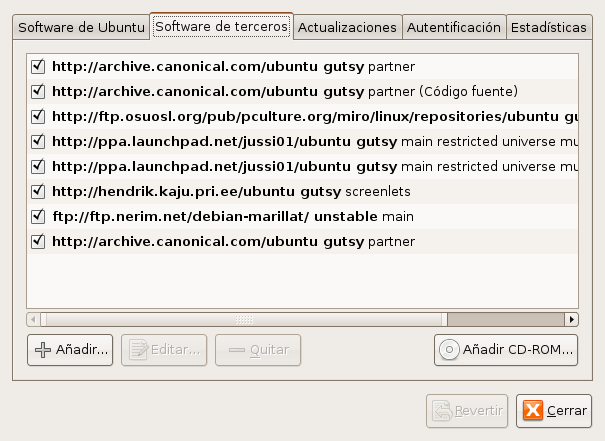
\includegraphics[width=.5\textwidth]{manuales/pestFuentes.png}
\caption{Pesta�a de Software de Terceros}
\label{pestFuentes}
\end{figure} Pulsaremos en el bot�n \command{A�adir} una primera vez, y pegaremos la siguiente l�nea: 

\begin{alltt}
deb http://\emph{tunombre.deservidor.org}/ubuntu gutsy main
\end{alltt}

 Volvemos a pulsarlo, y ahora introducimos �sta, correspondiente a un repositorio de paquetes de c�digo fuente (de ah� el \emph{deb-src}): 

\begin{alltt}
deb-src http://\emph{tunombre.deservidor.org}/ubuntu gutsy main
\end{alltt}

 Cambiamos a la pesta�a \emph{Autentificaci�n}, que ser� parecida a la de la figura , y pulsamos \command{Importar clave}. Seleccionaremos el fichero \filename{claveDebian.asc} antes descargado. 

\begin{figure}
\centering
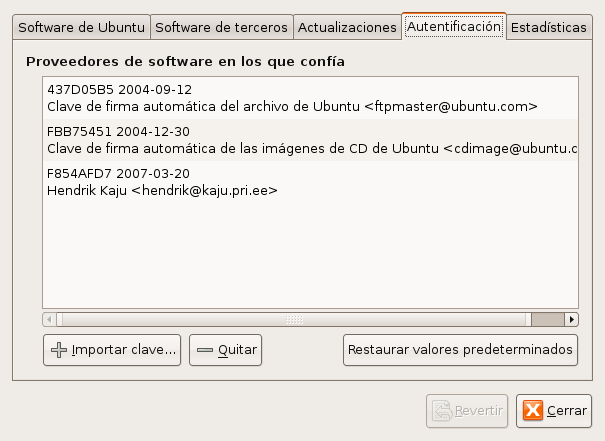
\includegraphics[width=.5\textwidth]{manuales/pestAutentificacion.png}
\caption{Pesta�a de Autentificaci�n}
\label{pestAutentificacion}
\end{figure} Guardamos los cambios realizados pulsando \command{Cerrar}, y finalmente pulsamos el bot�n \command{Recargar} de la barra de herramientas de la ventana principal. Cuando se cierre autom�ticamente el di�logo que aparece, ya podremos usar como siempre \application{Synaptic}, empleando el bot�n \command{Buscar} para hallar el paquete que deseamos, marcarlo con un doble clic e instalarlo mediante \command{Aplicar}. Adem�s, a partir de ahora, el sistema \application{apt} se ocupar� de monitorizar dicho repositorio y mantener actualizado el sistema. 

\section{Creaci�n y mantenimiento del paquete}

 En este cap�tulo, dar� un ejemplo de un paquete razonablemente sencillo, pero completo: un emulador de SNES, conocido como ZSNES. Veremos todas las fases, desde que nos descargamos el c�digo fuente hasta que tenemos el paquete instalado en nuestro sistema y funcionando. Existen muchas gu�as de creaci�n de paquetes, pero en mi opini�n la informaci�n se halla bastante fragmentada. De todas formas, en el wiki de Ubuntu hay una excelente introducci�n acerca del tema~\cite{packagingcomplete}, y tambi�n hay una gu�a por parte de la comunidad Debian~\cite{debianmaintainer}, aunque en mi opini�n la de Ubuntu est� m�s actualizada. 

 Para simplificar, describir� el proceso de forma secuencial. Sin embargo, lo normal es que sea iterativo, teniendo muchas revisiones intermedias del paquete hasta dejarlo listo para su distribuci�n. Se ven aspectos m�s avanzados en el siguiente cap�tulo. 

\subsection{Adaptaciones previas al uso de Subversion}

\subsubsection{Creaci�n de un esqueleto}

 Antes de poder introducir los ficheros fuente de nuestro paquete en el repositorio Subversion que previamente preparamos, hemos de crear una primera versi�n de nuestro paquete. 

 Tras descargar el c�digo fuente de la p�gina
	oficial (\url{http://www.zsnes.com/index.php?page=files}) a \filename{/tmp/\-packages/\-zsnes151src.tar.bz2}, crearemos el esqueleto b�sico del paquete mediante \command{dh\_make}, una de las muchas herramientas del paquete \application{debhelper} de ayuda. Ejecutaremos las siguientes �rdenes en una terminal dentro del directorio \filename{/tmp/\-packages}: 

\begin{alltt}
tar -xjf zsnes151src.tar.bz2
mv zsnes\_1\_51 zsnes-1.510
cd zsnes-1.510
dh\_make -e \emph{tudireccion@decorreo} -c GPL -s --createorig
      
\end{alltt}

 La carpeta que hemos creado (\filename{zsnes-1.510}) obedece al convenio seguido por Debian \filename{nombrepaquete-versionUpstream}, donde la versi�n del programa original se entiende como una serie de n�meros separados por puntos: as�, \filename{zsnes-1.510} es m�s reciente que \filename{zsnes-1.6}, y menos que \filename{zsnes-1.600}. 

 Por otro lado, las opciones pasadas a \command{dh\_make} son: 

\begin{description}
\item[-e tudireccion@decorreo] \mbox{}
 Especifica nuestra direcci�n email como desarrollador del paquete. Se usa en el registro de cambios (de ahora en adelante el \emph{Changelog}), y para realizar firmas digitales. 

\item[-c GPL] \mbox{}
 Indica que el c�digo original sigue la General Public License. Otras opciones incluyen la LGPL, BSD o la licencia art�stica. En otro caso, se nos dejar� un hueco (posteriormente veremos d�nde) para que lo rellenemos con el texto de la licencia en cuesti�n. 

\item[-s] \mbox{}
 Existen varios tipos de paquete Debian: de un solo binario, de varios, bibliotecas, o paquetes que emplean CDBS (el resto usan �nicamente \application{debhelper}). Aqu� hemos decidido hacer un paquete de un solo binario, mediante debhelper. Despu�s veremos tambi�n c�mo hacer un paquete con CDBS. 

\item[--createorig] \mbox{}
 Creamos en el directorio padre un fichero \filename{zsnes\_1.510.orig.tar.gz} con el c�digo fuente original, para poder comparar con la versi�n que usemos al construir el paquete y volcar las diferencias a un fichero \filename{diff}. 

\end{description}

\subsubsection{Edici�n}

 Ya tenemos el esqueleto del paquete. Todos los ficheros espec�ficos de �l se hallan bajo el directorio \filename{/tmp/\-packages/\-zsnes-1.510/\-debian}. Si examinamos dicho directorio, veremos que hay un gran n�mero de ficheros. No utilizaremos los ejemplos incluidos, indicados por la extensi�n \filename{.ex}, as� que los retiraremos, junto con el fichero \filename{README.Debian}, dado que no hay nada especial acerca de nuestro paquete: 

\begin{alltt}
rm debian/*.{ex,EX} debian/README.Debian
\end{alltt}

 Iremos rellenando cada fichero de control en \filename{debian} con los datos necesarios. Iremos detallando su sintaxis y sem�ntica a lo largo de esta secci�n. 

\paragraph{changelog}

 �ste es el registro de cambios de nuestro paquete. Aqu� iremos indicando los cambios realizados a lo largo de cada versi�n del paquete, no del software original. Este fichero es el que nuestros usuarios leer�n para ver qu� hay de nuevo en cada versi�n del paquete. 

 Escribiremos nuestra primera entrada: 

{ \small
\begin{alltt}
zsnes (1.510-0ubuntu1) gutsy; urgency=low

  * Versi�n inicial del paquete

 -- Antonio Garcia <nyoescape@gmail.com>  Fri, 19 Feb 2008 13:49:12 +0100
\end{alltt}
}

 Vemos c�mo la versi�n actual del paquete junto con su �ltima fecha y autor del cambio se hallan codificados en el registro. Tambi�n se tiene en cuenta la distribuci�n (en nuestro caso \emph{gutsy}, de Ubuntu), y la urgencia del cambio (por lo general baja, a menos que se trata de una vulnerabilidad de seguridad o algo del estilo). 

 Para una misma versi�n del software original, tendremos distintas versiones del paquete, separadas del n�mero de versi�n original por un gui�n, como vemos aqu�. En particular, los paquetes de Ubuntu~\cite{ubuntuversioning} usan el esquema \varname{-XubuntuY}, indicando que se trata de la Y-�sima versi�n del paquete de Ubuntu originado de la X-�sima versi�n del paquete Debian (0 si no proviene de un paquete Debian). Los n�meros de versi�n de paquete comienzan por 1. 

\note{ La raz�n de este esquema de versionado es para permitir una f�cil integraci�n con los paquetes Debian. Normalmente, la pol�tica de Ubuntu es s�lo crear nuevos paquetes o versiones de �stos si el paquete Debian est� anticuado o tiene alg�n problema. As�, si los de Debian sacan una nueva versi�n, como la \varname{-3}, a partir de \varname{-2ubuntu3}, se reflejar� dicha informaci�n de forma correcta. }

 As�, para la pr�xima versi�n del paquete, s�lo tendremos que a�adir la entrada en cuesti�n al registro, y nuestros guiones de ayuda har�n el resto del trabajo. 

\note{ Mucho cuidado con el formato del registro, es muy r�gido. El espaciado debe ser exactamente el mismo que en el ejemplo, como los dos espacios entre la direcci�n de correo y la fecha, o el espacio inicial al inicio de la misma l�nea. }

\paragraph{compat}

 Para este fichero no hay que hacer nada: s�lo contiene un n�mero entero, indicando qu� versi�n del paquete \application{debhelper} estamos usando. 

\paragraph{control}

 Este fichero es muy importante: describe todos los paquetes que estamos definiendo y enuncia sus dependencias. El formato es tambi�n bastante r�gido, pero muy simple. Utiliza una serie de campos delimitados por ':' y saltos de l�nea. 

 Por supuesto, no existe ninguna receta m�gica que nos diga las dependencias de un programa cualquiera. Para ello, normalmente tendremos que examinar la documentaci�n del desarrollador original, y/o el gui�n de compilaci�n que utilice: como aqu� usan las \application{autotools}, podr�amos consultar \filename{src/\-configure.in}. Una buena referencia respecto a las \application{autotools} es el Autobook~\cite{autobook}. 

 Por suerte, los desarrolladores de ZSNES han incluido dichas dependencias en \filename{docs/\-install.txt}, con lo que no tendremos que ir buscando en los guiones de compilaci�n. 

 El fichero que usaremos ser� �ste: 

\begin{alltt}
Source: zsnes
Section: games
Priority: optional
Maintainer: Antonio Garcia <nyoescape@gmail.com>
Build-Depends: cdbs, debhelper (>= 4.1.0), autotools-dev, fakeroot, 
  desktop-file-utils, g++ (>= 4), libsdl1.2-dev, nasm (>= 0.98), 
  zlib1g-dev (>= 1.2.3), libpng12-dev (>= 1.2), libncurses5-dev, 
  libgl1-mesa-dev
Standards-Version: 3.7.2

Package: zsnes
Architecture: i386
Depends: \${shlibs:Depends}
Description: Emulador de Super Nintendo
 Emulador de la consola Super Nintendo con m�s funciones 
 disponibles. Permite guardar y cargar estados, grabar 
 demostraciones, y aplicar diversos filtros. Tiene una 
 compatiblidad inmejorable.
\end{alltt}

\note{ En �ste y en cualquier otro fichero de control de Debian, no debemos olvidar poner un salto de l�nea justo al final del fichero. }

 Examinando el fichero de campo a campo, tenemos: 

\begin{description}
\item[\computeroutput{Source: zsnes}] \mbox{}
Indica que el paquete fuente del que derivan todos se llama "zsnes".

\item[\computeroutput{Section: games}] \mbox{}
Por la pol�tica de Debian~\cite{debianpolicy}, todo paquete se halla en alguna secci�n de las disponibles. As� indicamos qu� tipo de aplicaci�n es: un juego, un editor, etc.

\item[\computeroutput{Priority: optional}] \mbox{}
 Indica la importancia del paquete: desde imprescindibles (\emph{required}), pasando por importantes (\emph{important}), est�ndar (\emph{standard}), opcionales (\emph{optional}), y extra (tienen conflicto con alguno de m�s prioridad). 

\item[\computeroutput{Maintainer: Antonio Garcia <nyoescape@gmail.com>}] \mbox{}
Nombre y direcci�n de contacto del desarrollador del paquete.

\item[\computeroutput{Build-Depends: ...}] \mbox{}
Paquetes requeridos para poder compilar este paquete. Incluye las herramientas para paquetes Debian y las dependencias del propio programa.

\item[\computeroutput{Standards-Version: 3.7.2}] \mbox{}
 Versi�n de la pol�tica de Debian que este documento sigue. Realmente se halla compuesta por varios documentos, todos situados bajo el directorio \filename{/usr/\-share/\-doc/\-debian-policy}. 

\item[\computeroutput{Package: zsnes}] \mbox{}
Nombre de uno de los paquetes binarios generados a partir del fuente. Aqu� s�lo hay uno y tiene el mismo nombre.

\item[\computeroutput{Architecture: i386}] \mbox{}
Arquitectura a la que va dirigida el paquete. Existe una gran variedad de valores, pero nos interesan sobre todo \emph{i386} (la IA-32 habitual), \emph{source} (c�digo fuente) y \emph{all} (c�digo sin una arquitectura definida, como programas Java, o guiones de alg�n lenguaje interpretado como Perl o Python).

\item[\computeroutput{Depends}] \mbox{}
 Paquetes requeridos para que �ste se instale y funcione correctamente. La variable \varname{\$\{shlib:Depends\}} incluye las dependencias deducidas de forma autom�tica en cuanto a bibliotecas din�micas se refiere. 

\item[\computeroutput{Description}] \mbox{}
Incluye una descripci�n corta de una sola l�nea y otra m�s larga de varias l�neas del contenido del paquete. Al igual que siempre, su formato es muy r�gido: toda l�nea de la descripci�n larga comienza por un espacio, y l�neas vac�as �nicamente a�aden un punto ('.'). El campo termina tras la primera l�nea sin dicho espacio inicial.

\end{description}

\note{ Mucho cuidado con los acentos y dem�s en el nombre del desarrollador del paquete y otros campos: podr�an causar problemas en el interior de la jaula \application{chroot}, que s�lo tiene soporte para los caracteres ASCII de 7 bits. }

\paragraph{copyright}

 Contiene la informaci�n relativa a la licencia del paquete y del programa original, junto con datos acerca de los autores originales, su copyright y de d�nde descargamos el c�digo fuente. 

 En este caso s�lo tenemos que rellenar sin m�s los campos. No se fuerza ning�n formato particular sobre el fichero. Es importante sustituir "Upstream Author(s)" por "Upstream Authors" y fijarnos en la informaci�n en \filename{docs/\-authors.txt} del c�digo fuente, o los verificadores de paquetes que veremos despu�s dar�n avisos al respecto. 

\paragraph{dirs}

 En este fichero listamos los directorios en que vamos a instalar alg�n fichero. Si no lo listamos aqu�, dicho directorio no va a hallarse disponible durante la construcci�n del paquete, as� que hay que tener cuidado. Las rutas deben de seguir el Filesystem Hierarchy Standard (FHS), disponible a trav�s de la orden \command{man hier} desde cualquier terminal. 

 Algunas rutas importantes y sus contenidos son: 

\begin{description}
\item[\filename{/bin}] \mbox{}
Ejecutables usados en modo monousuario. Normalmente realizan tareas de mantenimiento a bajo nivel, entre otras cosas. Instalados a trav�s de paquetes Debian.

\item[\filename{/boot}] \mbox{}
Configuraci�n de GRUB, ficheros de imagen de los \emph{kernels} disponibles, etc.

\item[\filename{/dev}] \mbox{}
�rbol de directorios donde cada dispositivo conectado al sistema es un fichero.

\item[\filename{/etc}] \mbox{}
Ficheros de configuraci�n global (para todos los usuarios).

\item[\filename{/home}] \mbox{}
Directorios de casa de cada usuario, con espacio para cada uno de ellos.

\item[\filename{/mnt}] \mbox{}
Dispositivos externos montados temporalmente: particiones de Windows, CD, DVD, pendrives, etc.

\item[\filename{/proc}] \mbox{}
�rbol de directorios con informaci�n del \emph{kernel} en cada fichero: procesos en ejecuci�n, dispositivos disponibles, etc.

\item[\filename{/root}] \mbox{}
Directorio de casa del superusuario.

\item[\filename{/sbin}] \mbox{}
Ejecutables para uso del superusuario.

\item[\filename{/usr}] \mbox{}
Datos, programas y bibliotecas compartidos por todos los usuarios.

\item[\filename{/usr/bin}] \mbox{}
Ejecutables para todos los usuarios, instalados a trav�s de paquetes Debian.

\item[\filename{/usr/lib}] \mbox{}
Bibliotecas para todos los usuarios, instalados a trav�s de paquetes Debian.

\item[\filename{/usr/local}] \mbox{}
Similar a \filename{/usr}, pero para uso del administrador.

\item[\filename{/usr/share}] \mbox{}
Datos compartidos por todos los usuarios.

\item[\filename{/usr/share/man}] \mbox{}
 P�ginas de \emph{man} disponibles. Toda p�gina se halla dentro de una secci�n. En particular, la de \application{zsnes} estar�a en la 1, tras ver las instrucciones disponibles a trav�s de la orden \command{man man}. 

\end{description}

 Dado que tenemos que instalar el ejecutable para todos los usuarios y una p�gina \emph{man}, nuestro fichero \filename{dirs} contendr�: 

\begin{alltt}
usr/bin
usr/share/man/man1	  
\end{alltt}

\note{ En este fichero, las rutas \emph{no} incluyen una barra inicial, como suelen hacer. Para ser m�s exactos, son rutas a crear dentro del �rea temporal de construcci�n del directorio \filename{debian/\-zsnes}, donde colocaremos todos los ficheros tal y como se descomprimir�n despu�s bajo el directorio ra�z, \filename{/}. }

\paragraph{\filename{rules}}

 Aqu� est� el fichero m�s importante de todos. Es el que decide qu� hay que hacer exactamente para compilar e instalar el paquete completo: documentaci�n, binarios, guiones y ficheros de datos. 

 De todas formas, en t�rminos generales, no es m�s que un \emph{makefile}, si bien uno que puede hacerse muy complejo: el objetivo \emph{build} compila, \emph{install} instala dentro del �rea de construcci�n del paquete, y \emph{clean} retira los ficheros generados durante la construcci�n. Esta �ltima se halla bajo la ruta relativa \filename{debian/\-zsnes} respecto del directorio principal del paquete. 

 Dado que escribir una y otra vez un \emph{makefile} completo para muchas aplicaciones parecidas era una p�rdida de tiempo, se han desarrollado diversos paquetes que factorizan cierta funcionalidad com�n, como instalar p�ginas \emph{man}, tipos MIME, entradas de men�, y cosas del estilo: son los guiones del paquete \filename{debhelper}. Pr�cticamente nadie hoy en d�a desarrolla sus paquetes sin estos guiones. 

 Algunos desarrolladores han decidido ir un paso m�s all�, y factorizar reglas para perfiles completos de aplicaciones. As�, si sabemos que se trata de una aplicaci�n desarrollada a trav�s de las autotools, s�lo tendremos que aplicar dicho perfil, a�adiendo las opciones oportunas que pasar a \filename{configure}, por ejemplo. Esto es el Common Debian Build System (CDBS)~\cite{cdbsdoc}, que usaremos en esta gu�a. Existen perfiles para aplicaciones Python, Perl, GNOME, KDE, Java (basadas en Ant), o incluso para aquellas con un simple \emph{makefile}. 

 Por supuesto, para paquetes complicados, este sistema se queda corto, pero son minor�a comparados con los dem�s. Adem�s, no es s�lo cuesti�n de simplicidad: factorizando la mayor proporci�n posible de reglas, blindaremos nuestro paquete ante cambios en la pol�tica de Debian en el futuro. 

 De todas formas, en general, la comunidad de desarrolladores se halla muy dividida entre usar o no CDBS: aunque factoriza mucha complejidad, resulta dif�cil de comprender y aprovechar en casos dif�ciles, a menos que seamos capaces de leer complejos ficheros \emph{makefile} por nosotros mismos, dado que no existe mucha documentaci�n detallada al respecto: para CDBS, el c�digo es la mejor documentaci�n. 

 Dado que resulta imposible entender bien CDBS si no se comprende antes el sistema tradicional, en esta secci�n explicaremos las dos alternativas. Comenzaremos por el sistema "tradicional" con los guiones de debhelper, y luego veremos c�mo CDBS factoriza la mayor parte de estas reglas. 

\subparagraph{Reglas con \application{debhelper}}

 Partiendo del esqueleto que autom�ticamente nos ha creado \command{dh\_make}, lo retocamos para este paquete en particular. Vamos a ver qu� tal ha quedado, y luego explicaremos qu� partes exactamente hemos cambiado, y por qu�: 

{ \lstset{language=make,basicstyle=\small}
\begin{lstlisting}[caption=Reglas de un paquete Debian creado con debhelper]
#!/usr/bin/make -f
# -*- makefile -*-

# This file was originally written by Joey Hess and Craig Small. As a
# special exception, when this file is copied by dh-make into a dh-make
# output file, you may use that output file without restriction.  This
# special exception was added by Craig Small in version 0.37 of dh-make.

# Uncomment this to turn on verbose mode.
#export DH_VERBOSE=1

# El c�digo se halla en un subdirectorio, no en la ra�z
SRCDIR = src
# Opciones a pasar a configure (--enable-release activa optimizaciones)
CONFIGURE_FLAGS = --disable-cpucheck --enable-release --with-x --with-opengl
# Opciones a usar en el compilador
CFLAGS = -Wall -g

ifneq (,$(findstring noopt,$(DEB_BUILD_OPTIONS)))
	CFLAGS += -O0
else
	CFLAGS += -O2
endif

configure: configure-stamp
configure-stamp:
	dh_testdir
	touch configure-stamp

build: build-stamp

build-stamp: configure-stamp 
	dh_testdir

	cd $(SRCDIR) && \
          force_arch=i586 ./configure $(CONFIGURE_FLAGS) --prefix=/usr
	$(MAKE) -C $(SRCDIR)

	touch $@

clean:
	dh_testdir
	dh_testroot
	rm -f build-stamp configure-stamp

	# Limpiamos tambi�n las herramientas internas usadas por ZSNES en su
	# compilaci�n
	-$(MAKE) -C $(SRCDIR) clean tclean
	# Borramos los ficheros temporales generados por la compilaci�n
	$(RM) $(SRCDIR)/tools/depbuild $(SRCDIR)/config.{log,status,h} $(SRCDIR)/Makefile

	dh_clean 

install: build
	dh_testdir
	dh_testroot
	dh_clean -k 
	dh_installdirs

	$(MAKE) -C $(SRCDIR) install DESTDIR=$(CURDIR)/debian/zsnes

# Build architecture-independent files here.
binary-indep: build install
# We have nothing to do by default.

# Build architecture-dependent files here.
binary-arch: build install
	dh_testdir
	dh_testroot
	dh_installchangelogs 
	dh_installdocs
	dh_installexamples
#	dh_install
#	dh_installmenu
#	dh_installdebconf	
#	dh_installlogrotate
#	dh_installemacsen
#	dh_installpam
#	dh_installmime
#	dh_python
#	dh_installinit
#	dh_installcron
#	dh_installinfo
	dh_installman $(SRCDIR)/linux/zsnes.1
	dh_link
	dh_strip
	dh_compress
	dh_fixperms
#	dh_perl
#	dh_makeshlibs
	dh_installdeb
	dh_shlibdeps
	dh_gencontrol
	dh_md5sums
	dh_builddeb

binary: binary-indep binary-arch
.PHONY: build clean binary-indep binary-arch binary install configure
\end{lstlisting}%$
}

 Aunque es bastante largo, conceptualmente es sencillo, gracias al uso de \application{debhelper}. Un par de cosas a destacar: 

\begin{enumerate}
\item  Dado que nuestro c�digo fuente se halla bajo un subdirectorio y no en el directorio ra�z del paquete, a�adimos una variable \varname{SRCDIR}, cuyo valor tendremos en cuenta para realizar un cambio de directorio antes de cada orden de compilaci�n. 

\item  Por otro lado, \varname{CURDIR} contiene la ruta del directorio ra�z actual desde el cual se est� construyendo el paquete. La ruta \filename{\$(CURDIR)/debian/\-zsnes} contiene un �rbol de directorios que sigue el FHS, y se corresponde con los ficheros contenidos en el paquete \filename{zsnes}. 

\item  Bajo el objetivo de compilaci�n \varname{build-stamp} a�adimos las �rdenes requeridas para compilar: invocamos al gui�n \filename{configure} con las opciones necesarias e iniciamos la compilaci�n. La opci�n \option{-C} pasada a \command{make} hace el cambio de directorio antes de comenzar, justo como \command{cd} hace para las dem�s. Hay que hacerlo para cada orden y no al principio debido al hecho de que tras cada orden volvemos al directorio original, al restaurarse el estado anterior del shell. 

\item  Repetimos el cambio en la invocaci�n a \command{make} para los otros objetivos \varname{clean} e \varname{install}. Puede verse c�mo se pasa la variable de entorno \varname{DESTDIR} con la ruta al �rea de construcci�n para la instalaci�n: evidentemente, el \emph{makefile} debe de estar hecho para tener esto en cuenta. Tenemos la suerte para este paquete de que ya sea as�: de lo contrario, tendr�amos que adaptar dicho fichero, �y posiblemente el resto del programa! 

\item  Por �ltimo, en el objetivo \varname{binary-arch} tenemos una serie de llamadas a distintos guiones de \application{debhelper}. Comentaremos y descomentaremos seg�n nos haga falta: as�, por ejemplo, un programa escrito en Perl no necesita \command{dh\_link} ni \command{dh\_strip}, al no generar ejecutables. 

 Hemos a�adido un argumento a \command{dh\_installman} con la p�gina \application{man} que queremos que se instale. Al igual que con todo lo dem�s, si no hubiera una, tendr�amos que crearla nosotros. Lo m�s usual en este caso es escribir un fichero SGML o XML DocBook y transformarlo a \emph{nroff} (el formato de las p�ginas \application{man}) mediante \application{docbook-to-man} o una hoja de estilos XSLT, por ejemplo. Podr�amos partir del ejemplo creado antes por \command{dh\_make}>, \filename{zsnes.sgml.ex}. 

\end{enumerate}

 Un detalle importante: la mayor�a de los guiones suponen que los ficheros bajo nuestro directorio \filename{debian} siguen una serie de convenciones. Por ejemplo, \command{dh\_installdocs} supone que existe alg�n fichero \filename{debian/\-zsnes.docs} o \filename{debian/\-docs} que liste la documentaci�n a instalar. En este caso, aprovechamos la documentaci�n que ya trae ZSNES, con lo que tendr�amos esto en \filename{debian/\-docs}: 

\begin{alltt}
docs/srcinfo.txt
docs/README.SVN
docs/opengl.txt
docs/stdards.txt
docs/authors.txt
docs/todo.txt
docs/install.txt
docs/thanks.txt
docs/support.txt
docs/README.LINUX
docs/readme.txt/about.txt
docs/readme.txt/faq.txt
docs/readme.txt/history.txt
docs/readme.txt/gui.txt
docs/readme.txt/advanced.txt
docs/readme.txt/index.txt
docs/readme.txt/games.txt
docs/readme.txt/netplay.txt
docs/readme.txt/readme.txt
docs/readme.txt/support.txt
docs/readme.htm/styles/release.css
docs/readme.htm/styles/print.css
docs/readme.htm/styles/jipcy.css
docs/readme.htm/styles/radio.css
docs/readme.htm/styles/corner.png
docs/readme.htm/styles/plaintxt.css
docs/readme.htm/styles/shared.css
docs/readme.htm/images/zsneslogo.png
docs/readme.htm/images/netplay.png
docs/readme.htm/images/quick.png
docs/readme.htm/images/saveslot.png
docs/readme.htm/images/cheat.png
docs/readme.htm/images/gui.png
docs/readme.htm/images/config.png
docs/readme.htm/images/game.png
docs/readme.htm/images/f1\_menu.png
docs/readme.htm/images/misc.png
docs/readme.htm/netplay.htm
docs/readme.htm/about.htm
docs/readme.htm/games.htm
docs/readme.htm/advanced.htm
docs/readme.htm/gui.htm
docs/readme.htm/support.htm
docs/readme.htm/readme.htm
docs/readme.htm/history.htm
docs/readme.htm/license.htm
docs/readme.htm/faq.htm
docs/readme.htm/index.htm
docs/readme.1st
\end{alltt}

\note{ Hemos usado ya otro fichero m�s del mismo estilo: \filename{dirs} es realmente el fichero que \command{dh\_installdirs} utiliza, por ejemplo. }

\subparagraph{Reglas con CDBS}

 Ahora que ya sabemos cu�l es la estructura real de un fichero de reglas, lo reescribiremos empleando CDBS: 

\begin{lstlisting}[caption=Reglas de un paquete Debain creadas utilizando CDBS]
#!/usr/bin/make -f
# -*- makefile -*-

DEB_SRCDIR = src

include /usr/share/cdbs/1/rules/debhelper.mk
include /usr/share/cdbs/1/class/autotools.mk

DEB_CONFIGURE_SCRIPT_ENV   += force_arch=i586
DEB_CONFIGURE_EXTRA_FLAGS   = --disable-cpucheck --with-x \
  --enable-release --with-opengl
DEB_INSTALL_MANPAGES_zsnes += $(DEB_SRCDIR)/linux/zsnes.1
\end{lstlisting}%$

 Sorprendentemente, esto es todo: ocho l�neas. Los dos \command{include} se ocupan de importar los conjuntos de reglas de apoyo para el uso interno de \application{debhelper} e implementar el soporte para el perfil de las autotools, respectivamente. 

 A continuaci�n, pasamos las mismas opciones a \filename{configure} que antes: pedimos que compile para Pentium o superior, que emplee aceleraci�n 3D y un interfaz gr�fico, optimice algo m�s de lo normal (\verb#--enable-release#) y no intente autodetectar nuestra CPU. Finalmente, indicamos que instale la p�gina man \filename{src/\-linux/\-zsnes.1} que incluye ZSNES. 

 Usaremos esta versi�n de \filename{debian/\-rules} para realizar el resto del documento, aprovechando algunas funcionalidades adicionales que aporta. Sin embargo, internamente, es exactamente lo mismo de antes. 

\subsubsection{Construcci�n preliminar}

 Con todo listo, ya podemos construir el paquete. Situ�ndonos en el directorio principal del paquete, \filename{/tmp/\-packages/\-zsnes-1.510}, ejecutaremos: 

\begin{alltt}
dpkg-buildpackage -rfakeroot
\end{alltt}

 Tras un cierto tiempo, nos preguntar� la contrase�a de nuestra clave privada para firmar el paquete de forma autom�tica. Poco despu�s, tendremos en \filename{/tmp/\-packages} nuestra primera versi�n del paquete Debian, \filename{zsnes\_1.510-0ubuntu1\_i386.deb}, junto con un fichero \filename{.dsc} que describe el paquete fuente que tambi�n hemos construido, y un \filename{diff.gz} con las diferencias respecto a las fuentes originales. 

\subsubsection{Inyecci�n en el repositorio}

 Con nuestra primera versi�n del paquete lista, s�lo nos queda inyectar el paquete en el repositorio Subversion. Nos situaremos en \filename{\~{}/\-packages} y ejecutaremos: 

\begin{alltt}
svn-inject -c2 -o /tmp/packages/zsnes\_1.510-0ubuntu1.dsc \textbackslash{}
  file:///home/\emph{tunombredeusuario}/.svnDebian
\end{alltt}

 Tras un cierto tiempo, ya tendremos enviado al repositorio central nuestro paquete, y nuestra copia de trabajo habr� sido creada, con lo que no necesitaremos m�s \filename{/tmp/\-packages}. 

 La opci�n \option{-o} evita que se guarde el c�digo fuente en el repositorio, usando �nicamente archivos \filename{tar.gz} en el subdirectorio \filename{tarballs} del directorio principal del repositorio, que no se hallar� bajo control de versiones. 

 El repositorio creado tiene la siguiente estructura: 

\begin{description}
\item[\filename{\~{}/packages/tarballs}] \mbox{}
 Contiene los ficheros \filename{tar.gz} con las fuentes originales de nuestros paquetes. 

\item[\filename{\~{}/packages/zsnes/build-area}] \mbox{}
 Se trata del directorio destino en el que se depositar�n todos los paquetes y dem�s ficheros que vayamos produciendo. 

\item[\filename{\~{}/packages/zsnes/branches}] \mbox{}
 Almacena las distintas ramas de desarrollo. Normalmente contendr�a las distintas versiones del c�digo original, pero al usar tarballs, es pr�cticamente in�til en nuestro caso. 

\item[\filename{\~{}/packages/zsnes/tags}] \mbox{}
 Permite asociar n�meros de versi�n con determinadas revisiones del repositorio. Posteriormente veremos c�mo se usa. 

\item[\filename{\~{}/packages/zsnes/trunk}] \mbox{}
 Aqu� se almacena la versi�n actual del paquete. S�lo almacenamos el directorio \filename{debian}, para ahorrar la complejidad y tiempo de descarga necesario de otra forma. 

\end{description}

\subsection{Preparaci�n de una primera versi�n}

\subsubsection{Construcci�n definitiva}

 Es el momento de reconstruir el paquete, pero esta vez haciendo uso de la jaula \application{chroot}, para asegurar que efectivamente hemos listado todas las dependencias correctamente. 

 Dado que la orden es bastante larga, lo mejor es a�adir un alias a dicha orden, o mejor a�n, declarar una funci�n de \application{dash} (la versi�n reducida del shell \application{bash} de Ubuntu) que haga dicha tarea, en \filename{\~{}/.bashrc}. A�adiremos estas l�neas: 

\begin{alltt}
function svn-b () {
  buildarea="`pwd`/../build-area";
  sudo cowbuilder --update
  svn-buildpackage  \textbackslash{}
    --svn-builder="pdebuild --auto-debsign --buildresult \${buildarea}" \textbackslash{}
    --svn-postbuild="rm \${buildarea}/*\_source.changes";
}

function svn-tag () {
  svn-buildpackage --svn-only-tag
}
\end{alltt}

 Nos situaremos en \filename{\~{}/packages/\-zsnes/\-trunk} y ejecutaremos: 

\begin{alltt}
svn-b
\end{alltt}

 Tras un tiempo prudencial, e introducir nuestras contrase�as de GPG y superusuario, tendremos una primera versi�n del paquete, comprobada dentro de una jaula \application{chroot}. 

\subsubsection{Verificaci�n}

 Sin embargo, no basta con que se compile e instale correctamente. Adem�s, el paquete debe de cumplir todas las pol�ticas de Debian, como pertenecer a un determinado conjunto de secciones, tener todos sus ficheros de control bien escritos, respetar el est�ndar FHS que antes mencionamos, etc. 

 De hecho, si queremos que nos lleguen a aceptar cualquier paquete en un repositorio Debian oficial, como la secci�n \emph{universe} o \emph{multiverse} de Ubuntu, o la secci�n \emph{unstable} o \emph{testing} de Debian, lo mejor que podemos hacer para evitar hacer perder tiempo a nuestro supervisor o supervisores (que ser�n los que efectivamente suban al repositorio el paquete las primeras veces) es pasar antes nuestro paquete por los dos verificadores disponibles: Linda y Lintian, y retirar todos los avisos. 

\note{ Seg�n parece, Linda, escrito en Python, es m�s reciente que Lintian, y tambi�n m�s r�pido. Por otro lado, Lintian est� escrito en Perl. Aparte de eso, no hay muchas diferencias: simplemente ejecutaremos ambos por seguridad, ya que tampoco supone un esfuerzo adicional considerable. }

 Lanzaremos los verificadores sobre el \filename{.deb}, que se hallar� en \filename{\~{}/packages/\-zsnes/\-build-area}, pidiendo explicaciones de los avisos y errores con \option{-i}: 

\begin{alltt}
linda -i \~{}/packages/zsnes/build-area/zsnes\_1.510-0ubuntu1\_i386.deb
lintian -i \~{}/packages/zsnes/build-area/zsnes\_1.510-0ubuntu1\_i386.deb
\end{alltt}

 Seg�n parece, no todo est� bien en nuestro paquete: 

{ \small
\begin{alltt}
W: zsnes: extra-license-file usr/share/doc/zsnes/license.htm
N:
N:   All license information should be collected in the debian/copyright
N:   file. This usually makes it unnecessary for the package to install
N:   this information in other places as well.
N:   
N:   Refer to Policy Manual, section 12.5 for details.
N:
E: zsnes: FSSTND-dir-in-usr usr/man/
N:
N:   As of policy version 3.0.0.0, Debian no longer follows the FSSTND.
N:   
N:   Instead, the Filesystem Hierarchy Standard (FHS), version 2.3, is
N:   used. You can find it in /usr/share/doc/debian-policy/fhs/ .
N:
E: zsnes; Manual page zsnes.1.gz installed into /usr/man.
 The manual page shown is installed into the legacy location of
 /usr/man, where they should be installed into /usr/share/man.
E: zsnes; FSSTND directory /usr/man in /usr found.
 As of policy version 3.0.0.0, Debian no longer follows the FSSTND.
 Instead, the Filesystem Hierarchy Standard (FHS), version 2.1, is
 used. You can find it in /usr/share/doc/debian-policy/fhs/ .
E: zsnes; FSSTND directory /usr/man/man1 in /usr found.
W: zsnes; File /usr/share/doc/zsnes/license.htm is considered to be an
 extra license file.  The file shown above is considered to be another
 license file, where as the license for a package should be contained
 in the copyright file, which should be installed into
 /usr/share/doc/<pkg>.
\end{alltt}
}

 Analizando esta salida, vemos que hay cuatro problemas con nuestro paquete seg�n Linda, y dos seg�n Lintian. El primer problema es f�cil de tratar: hemos incluido un fichero de licencia con la documentaci�n (\varname{extra-license-file}), que no deber�a estar, ya que el archivo \filename{copyright} deber�a contener toda la informaci�n. Basta en este caso con retirar la l�nea problem�tica de \filename{debian/\-docs}. 

 El segundo problema es m�s complejo: el directorio \filename{/usr/\-man} no es parte del est�ndar actual, FHS, sino de uno m�s antiguo, el FSSTND (FileSystem Standard). En principio, nuestras reglas est�n bien escritas. Veamos si efectivamente nuestro paquete pone la p�gina man en su sitio: 

\begin{alltt}
\prompt{\~{}/packages/zsnes/trunk\$ dpkg \textbackslash{}
  -c ../build-area/zsnes\_1.510-0ubuntu1\_i386.deb}     
\end{alltt}

 S� que lo hace: \filename{/usr/\-share/\-man/\-man1/\-zsnes.1.gz} aparece como deber�a. Sin embargo, tambi�n aparece \filename{/usr/\-man/\-man1/\-zsnes.1.gz}. As�, hay algo fuera de nuestras reglas que est� instalando en dicho sitio la p�gina \application{man}. 

 Vamos a descomprimir en un directorio temporal el c�digo fuente original, y echar un vistazo con la inestimable ayuda de \application{grep}, empleando la opci�n \option{-R} para hacer una b�squeda recursiva por el �rbol de directorios y \option{-l} para solamente listar los ficheros con coincidencia y no el contenido que sigue el patr�n: 

\begin{alltt}
cd /tmp
tar -xzf \~{}/packages/tarballs/zsnes\_1.510.orig.tar.gz
cd zsnes-1.510.orig
grep -Rl zsnes.1 *
\computeroutput{docs/srcinfo.txt
docs/readme.txt/readme.txt
docs/readme.htm/readme.htm
src/Makefile.in}
\end{alltt}

 Ya lo hemos encontrado: descartando los tres ficheros que forman parte de la documentaci�n, s�lo queda \filename{src/Makefile.in}. Tiene que ser el culpable, ya que este fichero es usado por el gui�n \filename{configure} para crear el \emph{makefile} con el que hacer la compilaci�n e instalar el programa. 

 Veremos exactamente d�nde est� el problema, empleando la opci�n \option{-C} para ver un contexto de un determinado n�mero de l�neas alrededor de las apariciones: 

{ \small
\begin{alltt}
grep -C4 zsnes.1 src/Makefile.in
\computeroutput{install:
        @INSTALL@ -d -m 0755 \$(DESTDIR)/@prefix@/bin
        @INSTALL@ -m 0755 @ZSNESEXE@ \$(DESTDIR)/@prefix@/bin
        @INSTALL@ -d -m 0755 \$(DESTDIR)/@prefix@/man/man1
        @INSTALL@ -m 0644 linux/zsnes.1 \$(DESTDIR)/@prefix@/man/man1
uninstall:
        rm -f @prefix@/bin/\$(notdir @ZSNESEXE@) @prefix@/man/man1/zsnes.1

clean:
        rm -f \$(Z\_OBJS) \$(PSR) \$(PSR\_H) @ZSNESEXE@
tclean:
}
\end{alltt}
}

 Ya hemos encontrado las dos l�neas problem�ticas, al final del objetivo \varname{install}: crean el directorio e instalan la p�gina \application{man}. S�lo hay que quitarlas. Sin embargo, hay un problema: no podemos tocar el c�digo directamente, ya que no lo tenemos bajo control de versiones. Es m�s: no se considera buena pr�ctica, ya que en futuras versiones los desarrolladores originales podr�an arreglar ese problema, y se har�a dif�cil ver qui�n ha hecho qu� tras hacer unos cuantos cambios m�s. 

 Por eso, se considera buena pr�ctica emplear un sistema de parches para hacer este tipo de modificaciones. Algunas alternativas~\cite{packagingpatching} incluyen el m�s antiguo, \application{dpatch}, el m�s reciente (y aparentemente superior, seg�n los desarrolladores de SUSE) \application{quilt} y el que usaremos aqu�, \application{simple-patchsys}, que como su nombre indica, est� m�s inclinado hacia ser sencillo que ser potente. Sin embargo, nos basta para casos sencillos como �ste. 

 Para usarlo, a�adimos la l�nea que instala soporte para �l en \filename{debian/\-rules}, justo despu�s del primer \varname{include}: 

\begin{alltt}
include /usr/share/cdbs/1/rules/simple-patchsys.mk
\end{alltt}

 Pasaremos a crear el parche en s�. Para ello, tenemos que obtener el �rbol de fuentes tal y como lo ver�a \filename{debuild} antes de compilar, y no como lo tenemos ahora. Para ello, usaremos \command{svn-buildpackage}, no sin antes enviar nuestros otros cambios al repositorio (de otra forma, no nos dejar� seguir): 

{ \small
\begin{alltt}
\prompt{\~{}/packages/zsnes/trunk\$ svn commit -m \textbackslash{}
  "Integrado simple-patchsys del CDBS y corregido documentaci�n"}
\computeroutput{Enviando       trunk/debian/docs
Enviando       trunk/debian/rules
Transmitiendo contenido de archivos ..
Commit de la revisi�n 6.}
\prompt{\~{}/packages/zsnes/trunk\$ svn-buildpackage --svn-export}
\computeroutput{buildArea: /home/antonio/packages/zsnes/build-area
[...]
I: mergeWithUpstream property set, looking for upstream source tarball...
[...]
Exportaci�n completa.
rm -rf /home/antonio/packages/zsnes/build-area/tmp-0.00194501814349124
Build directory exported to /home/antonio/packages/zsnes/build-area/zsnes-1.510}
\end{alltt}
}

 Iremos al directorio exportado de construcci�n, que contendr� todos los ficheros necesarios, y generaremos el parche usando \command{cdbs-edit-patch}: 

\begin{alltt}
\prompt{\~{}/packages/zsnes/trunk\$ cd ../build-area/zsnes-1.510/}
\prompt{\~{}/packages/zsnes/build-area/zsnes-1.510\$ cdbs-edit-patch 01-man-fhs.patch}
\end{alltt}

 El programa nos indicar� que nos hallamos ahora en un subshell, y que hagamos las modificaciones necesarias. Usando un editor cualquiera, retiraremos dichas l�neas de \filename{src/\-Makefile.in}. Hecho esto, pulsaremos \texttt{CTRL + D} o introduciremos la orden \command{exit} para salir del subshell y dejar que cree el parche \filename{debian/\-patches/\-01-man-fhs.patch} con los cambios que hemos hecho. 

 S�lo hemos de colocar ahora el parche en el sitio correcto, y guardar los cambios en el repositorio: 

\begin{alltt}
cd \~{}/packages/zsnes/trunk
cp -r ../build-area/zsnes-1.510/debian/patches debian
svn add debian/patches
svn commit -m "Arreglado problema con la p�gina man en /usr/man"
\end{alltt}

 Ahora reconstruiremos el paquete: 

\begin{alltt}
svn-b
\end{alltt}

 Ya, por fin, Lintian y Linda no dan ning�n aviso. Probaremos a instalar el paquete, y ver qu� tal funciona: 

\begin{alltt}
sudo dpkg -i ../build-area/zsnes\_1.510-0ubuntu1\_i386.deb
\end{alltt}

 Tras probar un poco el emulador con alguna ROM libremente disponible, como las de PDRoms (\url{http://www.pdroms.com}), decidimos que el paquete est� en condiciones de ser usado. Usaremos la otra funci�n que definimos antes para marcar esta versi�n del paquete, copiando los contenidos de \filename{trunk} en un nuevo subdirectorio de \filename{tags} cuyo nombre ser� la versi�n actual del paquete, para despu�s confirmar los cambios que se habr�n realizado autom�ticamente en \filename{debian/changelog}, en preparaci�n para la siguiente versi�n de nuestro paquete: 

\begin{alltt}
svn-tag
svn commit -m "Copiado a tags versi�n 1.510-0ubuntu1 del paquete"
\end{alltt}

\subsubsection{Env�o al repositorio Debian}

 Despu�s de haber verificado nuestro paquete y haber marcado la versi�n en el repositorio Subversion, es momento de enviarlo al repositorio Debian, para que nuestros usuarios puedan acceder f�cilmente a �l. A�adiremos tanto el paquete fuente como el paquete compilado: 

\begin{alltt}
sudo -E reprepro includedeb gutsy \textbackslash{}
 \~{}/packages/zsnes/build-area/zsnes\_1.510-0ubuntu1\_i386.deb
sudo -E reprepro -S main -P low includedsc gutsy \textbackslash{}
 \~{}/packages/zsnes/build-area/zsnes\_1.510-0ubuntu1.dsc
\end{alltt}

 Deber�amos probar el paquete justo como un usuario normal lo har�a. Pero, primero, tenemos que desinstalar la versi�n que instalamos antes a partir de un fichero: 

\begin{alltt}
sudo aptitude remove zsnes
sudo aptitude update
sudo aptitude install zsnes
\end{alltt}

\subsection{Actualizaci�n del paquete a una nueva versi�n del programa}

 Cada cierto tiempo, deberemos de actualizar nuestro repositorio con los cambios realizados en el c�digo. Para ello, disponemos de la orden \command{svn-upgrade}, a la que le pasaremos un fichero \filename{tar.gz} con el nuevo c�digo fuente del paquete. 

 Ahora probaremos a actualizar nuestro paquete con el c�digo correspondiente a la �ltima versi�n en el repositorio Subversion del equipo de ZSNES. Primero, prepararemos el tarball con el c�digo original. Descargamos el c�digo fuente, y lo exportamos a otro directorio, para retirar los ficheros usados por \application{Subversion}: 

\begin{alltt}
svn checkout https://svn.bountysource.com/zsnes/trunk zsnes-svn
svn export zsnes-svn zsnes-1.510.SVN5215
\end{alltt}

 He decidido usar el esquema \varname{1.510.SVN5215} para indicar que se trata de la revisi�n 5215 del repositorio. De esta forma, si sale una nueva versi�n oficial, o si empleo una revisi�n m�s reciente del repositorio Subversion, como \varname{1.520} o \varname{1.510.SVN5216}, �stas ser�n considerada m�s recientes, y la actualizaci�n se podr� hacer de forma correcta. Podemos comprobar que es efectivamente as� mediante la siguiente orden: 

\begin{alltt}
dpkg --compare-versions "1.510-0ubuntu1" gt "1.510.SVN5215-0ubuntu1" \&\& \textbackslash{}
  echo "1.510-0ubuntu1 mayor que 1.510.SVN5215-0ubuntu1" || \textbackslash{}
  echo "1.510-0ubuntu1 menor que 1.510.SVN5215-0ubuntu1"
\end{alltt}

 Ahora que ya tenemos el c�digo, inspeccionaremos un momento para ver si todos los ficheros importantes se hallan en su sitio. Normalmente, no se suelen almacenar ficheros generados autom�ticamente en el repositorio, as� que pueden que falten algunas cosas importantes. Mirando en \filename{src}, vemos que falta el gui�n \filename{configure} que necesitamos para compilar. Lo generaremos ejecutando las siguientes �rdenes bajo \filename{src}, el mismo directorio donde se halla su fichero fuente, \filename{configure.in}: 

\begin{alltt}
aclocal
autoconf
\end{alltt}

 Tambi�n faltan los directorios \filename{docs/\-readme.txt} y \filename{docs/\-readme.htm}, que a�adiremos en su sitio. Con esto tenemos los ficheros fuente listos. Vamos a crear el tarball que necesitamos: 

\begin{alltt}
\prompt{/tmp\$ tar -czf zsnes-1.510.SVN5215.tar.gz zsnes-1.510.SVN5215}
\end{alltt}

 El siguiente paso es a�adir dicho c�digo a nuestra �rea de trabajo, e indicar que vamos comenzar a empaquetar una nueva versi�n del programa. Volvemos al directorio con la versi�n actual de nuestro paquete y ejecutamos: 

\begin{alltt}
\prompt{\~{}/packages/zsnes/trunk\$ svn-upgrade /tmp/zsnes-1.510.SVN5215.tar.gz}
\end{alltt}

 Se har�n los cambios necesarios en \filename{debian/\-changelog} y el resto del repositorio. Cambiaremos el n�mero de versi�n del paquete a \varname{0ubuntu1} y confirmamos dichos cambios antes de volver a reconstruir el paquete: 

\begin{alltt}
\prompt{\~{}/packages/zsnes/trunk\$ svn commit -m \textbackslash{}
  "Actualizado con rev 5215 upstream"}
\prompt{\~{}/packages/zsnes/trunk\$ svn-b}
\end{alltt}

 Sin embargo, la reconstrucci�n falla. Buscando entre los distintos mensajes, podemos ver una l�nea del estilo: 

\begin{alltt}
\computeroutput{Trying patch 01-man-fhs.patch at level 1 ... 0 ... 2 ... failed.}
\end{alltt}

 En resumen: el parche que antes hicimos para corregir el problema de \filename{Makefile.in} no se ha podido aplicar. Tras inspeccionar sus contenidos, vemos que efectivamente \filename{Makefile.in} ha cambiado demasiado: 

\begin{alltt}
install:
	@INSTALL@ -d -m 0755 \$(DESTDIR)/@bindir@
	@INSTALL@ -m 0755 @ZSNESEXE@ \$(DESTDIR)/@bindir@
	@INSTALL@ -d -m 0755 \$(DESTDIR)/@mandir@/man1
	@INSTALL@ -m 0644 linux/zsnes.1 \$(DESTDIR)/@mandir@/man1
\end{alltt}

 Vaya, parece que ellos mismos han corregido ya el problema que ten�amos antes. �sta es precisamente la raz�n por la que usamos un parche, en vez de cambiar directamente el c�digo. S�lo tenemos que eliminar el parche, confirmar los cambios y reconstruir: 

\begin{alltt}
\prompt{\~{}/packages/zsnes/trunk\$ svn rm debian/patches}
\computeroutput{D  debian/patches/01-man-fhs.patch}
\prompt{\~{}/packages/zsnes/trunk\$ svn commit -m \textbackslash{}
  "01-man-fhs.patch: Retirado (corregido por upstream)"}
\computeroutput{Deleting       zsnes/trunk/debian/patches/01-man-fhs.patch
Transmitting file data .
Committed revision 11.}
\prompt{\~{}/packages/zsnes/trunk\$ svn-b}
\end{alltt}

 Esta vez ya no da el fallo del parche, pero indica que faltan las bibliotecas de desarrollo de Qt para la nueva interfaz. A�adiremos la dependencia en \filename{libqt4-dev} al fichero \filename{control} y volveremos a intentarlo tras confirmar otra vez nuestros cambios. 

 Esta vez falla diciendo que no puede construir el fichero \filename{ui\_zsnes.h}, que hace falta para compilar. Probaremos a compilar sobre el directorio \filename{/tmp/zsnes-1.510.SVN5215/\-src} tras instalar las dependencias en nuestro propio sistema: 

\begin{alltt}
./configure
make
\end{alltt}

 Da el mismo problema, as� que no es culpa de nuestro paquete. Vamos a mirar con \application{grep}, a ver qu� puede ser: 

\begin{alltt}
\prompt{grep -R ui\_zsnes.h *}
\computeroutput{makefile.ms:\${GUI\_D}/gui.cpp: \${GUI\_D}/ui\_zsnes.h
src/gui/gui.h:\#include "ui\_zsnes.h"
Makefile.in:GUI\_QO=\$(GUI\_D)/moc\_gui.cpp \$(GUI\_D)/ui\_zsnes.h
Makefile:GUI\_QO=\$(GUI\_D)/moc\_gui.cpp \$(GUI\_D)/ui\_zsnes.h
makefile.dep:gui/gui.o: gui/gui.cpp gui/gui.h ui\_zsnes.h
}
\end{alltt}

 Si nos fijamos, se puede ver que en \filename{makefile.dep} la ruta no se corresponde con la de las anteriores entradas, por lo que seguramente ah� estar� el fallo. Esta vez buscamos por este fichero: 

{ \small
\begin{alltt}
\prompt{grep -R makefile.dep *}
\computeroutput{src/configure:touch -t 198001010000 makefile.dep
src/Makefile.in:main: makefile.dep \$(Z\_QOBJS) \$(Z\_OBJS)
src/Makefile.in:include makefile.dep
src/Makefile.in:makefile.dep: \$(TOOL\_D)/depbuild Makefile
src/Makefile.in: \$(TOOL\_D)/depbuild @CC@ "@CFLAGS@" @NASMPATH@
"@NFLAGS@" \$(Z\_OBJS) > makefile.dep
src/Makefile.in: rm -f makefile.dep \$(Z\_OBJS) \$(Z\_QOBJS) \$(PSR)
\$(PSR\_H) @ZSNESEXE@
src/Makefile:main: makefile.dep \$(Z\_QOBJS) \$(Z\_OBJS)
src/Makefile:include makefile.dep
src/Makefile:makefile.dep: \$(TOOL\_D)/depbuild Makefile
src/Makefile: \$(TOOL\_D)/depbuild gcc " -pipe -I. -I/usr/local/include
-I/usr/include -D\_\_UNIXSDL\_\_ -I/usr/include/SDL -D\_GNU\_SOURCE=1
-D\_REENTRANT -D\_\_OPENGL\_\_ -DNO\_DEBUGGER -DNDEBUG -march=athlon-xp -O2
-fomit-frame-pointer -s -DQT\_SHARED -I/usr/include/qt4
-I/usr/include/qt4/QtCore -I/usr/include/qt4/QtGui " nasm "
-w-orphan-labels -D\_\_UNIXSDL\_\_ -f elf -DELF -D\_\_OPENGL\_\_ -DNO\_DEBUGGER
-O1" \$(Z\_OBJS) > makefile.dep
src/Makefile: rm -f makefile.dep \$(Z\_OBJS) \$(Z\_QOBJS) \$(PSR) \$(PSR\_H)
zsnes
src/autom4te.cache/output.0:touch -t 198001010000 makefile.dep
src/autom4te.cache/output.1:touch -t 198001010000 makefile.dep
src/configure.in:touch -t 198001010000 makefile.dep
}
\end{alltt}
}

 Puede verse que en \filename{src/Makefile} es donde se crea a trav�s de una herramienta propia de los desarrolladores de ZSNES, que obtiene autom�ticamente las dependencias. Recordando la lista anterior de ficheros que mencionaban a \filename{ui\_zsnes.h}, se nos viene a la cabeza \filename{gui/\-gui.h}. Vamos a probar a cambiar la ruta de inclusi�n a \filename{gui/\-ui\_zsnes.h}: 

\begin{alltt}
cd \~{}/packages/zsnes/trunk
svn-buildpackage --svn-export
cd ../build-area/zsnes-1.510.SVN5215
cdbs-edit-patch 02-fix-depbuild.patch
\end{alltt}

 Hacemos el cambio antes mencionado con el editor \application{vim} y salimos del shell, tras lo cual reintentaremos la construcci�n del paquete: 

\begin{alltt}
vim src/gui/gui.h
exit
\end{alltt}

 Ahora la reconstrucci�n ha tenido �xito. Ya s�lo tendr�amos que seguir los mismos pasos anteriores de verificaci�n, validaci�n manual, marcado en el repositorio (tras retirar el aviso <<NOT RELEASED YET>> a�adido autom�ticamente a \filename{debian/changelog}, claro), y env�o. Cualquiera de nuestros usuarios ser� notificado eventualmente de la actualizaci�n y podr� instalar la versi�n m�s reciente del paquete. 

 Una �ltima nota: si se quiere, se puede integrar la verificaci�n y publicaci�n en la funci�n \command{svn-b} antes definida, cambiando las l�neas correspondientes en \filename{\~{}/.bashrc} por: 

\lstset{language=bash}
\begin{lstlisting}[basicstyle=\small,caption=Funciones Bash de ayuda para construcci�n de paquetes]
function svn-b () {
  buildarea="`pwd`/../build-area";
  rutapaquete="${buildarea}/\${package}_\${debian_version}*.deb";
  rutadsc="${buildarea}/\${package}_\${debian_version}*.dsc";
  rutarepo="/var/packages/ubuntu";
  sudo cowbuilder --update
  svn-buildpackage  \
    --svn-builder="pdebuild --auto-debsign --buildresult ${buildarea}" \
    --svn-postbuild="rm ${buildarea}/*_source.changes; \
            lintian -i ${rutapaquete}; linda -i ${rutapaquete}; \
            cd ${rutarepo} && \
            sudo -E reprepro remove gutsy \${package} && \
            sudo -E reprepro includedeb gutsy ${rutapaquete} && \
            sudo -E reprepro -S main -P low includedsc gutsy ${rutadsc}";
}
function svn-tag () {
  svn-buildpackage --svn-only-tag
}
\end{lstlisting}%$

\section{Otros aspectos de inter�s}

\subsection{Integraci�n de repositorio propio con la jaula \application{chroot}}

 En este tutorial no har� falta, pero s� es posible que nos haga falta para casos m�s complejos. Cuando haya interdependencias entre varios paquetes que deseemos crear, tendremos que a�adir nuestro repositorio (que estar� alojado en su propio servidor web) a la lista de los repositorios de la jaula \application{chroot}. 

 Para ello, nos introduciremos en la jaula e importaremos la firma digital de nuestros paquetes: 

\begin{alltt}
sudo cowbuilder --login --save-after-login
wget http://\emph{direccion.delservidor.org}/claveDebian.asc
apt-key add claveDebian.asc
\end{alltt}

 Con esto, la jaula ya confiar� en nuestros paquetes. Tenemos que a�adir entonces la siguiente l�nea a \filename{/etc/apt/sources.list}, usando el editor \application{vim}: 

\begin{alltt}
deb http://\emph{direccion.delservidor.org}/ubuntu gutsy main
\end{alltt}

 Actualizamos la lista de paquetes: 

\begin{alltt}
aptitude update
\end{alltt}

 Hemos terminado, as� que s�lo queda salir del shell de la jaula: 

\begin{alltt}
exit
\end{alltt}

\subsection{Sincronizaci�n de un repositorio en Internet con un repositorio local}

 En muchos casos no dispondremos de los medios necesarios como para dejar nuestro ordenador como servidor web al exterior para que sirva nuestros paquetes. En estos casos, podemos subir nuestros ficheros \filename{.deb} a una forja o algo del estilo y dejar que los usuarios se los bajen. 

 Pero, �y si son muchos paquetes, o si queremos mantener actualizados a los usuarios? Lo mejor ser�a replicar completo el repositorio en un servidor conectado permantentmente a Internet. La mejor opci�n es, por tanto, obtener espacio de alojamiento con acceso mediante SFTP o FTP. 

 Una vez lo hayamos conseguido, podr�amos subir el �rbol completo de directorios de nuestra m�quina al servidor remoto, pero hacer esto una y otra vez tardar�a demasiado. La mejor opci�n es hacer un \emph{mirror inverso} a trav�s de la herramienta \application{lftp}, que nos pedir� la contrase�a antes de conectarse: 

\begin{alltt}
lftp -d -e "mirror -venR \emph{ruta local} \textbackslash{}
                         \emph{ruta remota} \textbackslash{}
                         \emph{direcci�n del servidor}"
\end{alltt}

 Si queremos que no nos pregunte una y otra vez la contrase�a, siempre podemos a�adir l�neas como �stas a \filename{\~{}/.netrc}, cuidando de que s�lo sea legible por nosotros: 

\begin{alltt}
machine \emph{mi.servidor.com}
login \emph{minombredeusuario}
password \emph{micontrase�a}
\end{alltt}

\subsection{Adaptaci�n de aplicaciones Java}

 La principal diferencia al crear un paquete Java es, sin duda, el hecho de que, a pesar de tener que compilar, el paquete en s� no tiene ninguna arquitectura definida. Ello deber�a verse reflejado en \filename{debian/control}. 

 Adem�s, deber�a tener en \varname{Build-Depends} alg�n compilador de Java, y en \varname{Depends} el paquete virtual \filename{java2-runtime}, adem�s de una alternativa concreta, como la de Sun, \filename{sun-java6-jre}, o preferiblemente la basada en OpenJDK, \filename{icedtea-java7-jre}, usando el operador l�gico OR (\varname{|}). Los paquetes virtuales no a�aden ninguna funcionalidad: se limitan a hacer cosas como ayudarnos a instalar varios paquetes de una sola vez (us�ndolos en su campo \varname{Depends}), o permiti�ndonos usar un paquete cualquiera que nos provea de una cierta funcionalidad. 

 As�, si curioseamos en el paquete \filename{sun-java6-jre}, veremos que tiene a dicho paquete virtual en el campo \varname{Provides} (<<Proporciona>>): 

\begin{alltt}
\prompt{\$ aptitude show sun-java6-jre}
\computeroutput{Paquete: sun-java6-jre
[...]
Proporciona: java-virtual-machine, java1-runtime, java2-runtime
[...]}
\end{alltt}

 Si usamos el compilador de Sun en Build-Depends (paquete \filename{sun-java6-jdk}), habremos de cambiar nuestro \filename{.pbuilderrc} para que use un interfaz distinto de entrada, que nos deje aceptar los t�rminos de la DLJ de Sun. A�adimos estas l�neas: 

\begin{alltt}
\# Para poder aceptar la licencia DLJ
export DEBIAN\_FRONTEND="readline" 
\end{alltt}

 Adem�s de eso, tendremos como de costumbre que adaptar nuestro programa Java para que sea f�cilmente compilable de forma autom�tica, y para que se integre bien dentro del sistema. Un problema es que no deber�amos escribir rutas absolutas en el c�digo Java, o si no perderemos toda la transportabilidad que dese�bamos en un primer momento. La forma m�s f�cil de implementar lo que deseamos es simplemente utilizar variables de entorno o propiedades del sistema. 

 A veces no nos servir� cualquier JRE de los disponibles para ejecutar nuestro programa, y tendremos que prescindir de usar \filename{java2-runtime}. Es el caso usual de las aplicaciones basadas en Swing: el JRE por defecto en Gutsy, GCJ, s�lo implementa completamente SWT. Tendremos que hacer que el sistema instale y active otro JRE. 

 Para poder establecerlas de forma separada del programa Java antes de lanzarlo, lo que necesitamos es un gui�n de shell, que ser� el que instalaremos en \filename{/usr/bin}. El fichero \filename{.jar}, siguiendo la pol�tica de Debian, debe ir en \filename{/usr/share/java}. 

 El que sea f�cilmente compilable de forma autom�tica depende de qu� sistema hayamos estado usando. Si nos hemos basado en un IDE, seguramente aqu� tengamos problemas. Lo que deber�amos hacer es reescribir la fase de compilaci�n usando un gui�n para \application{Apache Ant}. Esto, de paso, nos permitir� aprovechar el perfil de CDBS, simplificando bastante nuestra tarea. \application{Ant} es efectivamente un sustituto del \application{GNU Make} escrito en Java, para aplicaciones Java. Utiliza ficheros muy del estilo de los \emph{makefile}, s�lo que escritos en XML. 

 Con todo esto, a�n hay un par de complicaciones adicionales. Normalmente, los ficheros fuente Java se hallan escritos en UTF-8. Sin embargo, la jaula \application{chroot} que antes hicimos en~\ref{paqueteslimpios} (p�gina~\pageref{paqueteslimpios}) no tiene en principio una localizaci�n compatible instalada. Vamos a tener que entrar en la jaula e instalar los paquetes necesarios, comprobando la situaci�n que aqu� describimos con \command{locale} (nos mostrar� que usamos la localizaci�n est�ndar <<C>>): 

\begin{alltt}
sudo cowbuilder --login --save-after-login
aptitude install language-pack-es
exit
\end{alltt}

 Ahora, lo que hemos de hacer es asegurarnos que cuando llamemos a \application{Ant}, lo hagamos estableciendo una localizaci�n con UTF-8: 

\begin{alltt}
LANG=es\_ES.UTF-8 ant compile
\end{alltt}

 Deber�amos adem�s invocar las pruebas de unidad sobre el c�digo, para asegurarnos de que el c�digo usado en el paquete no presente regresiones. Adem�s de a�adir el paquete \filename{junit} a \varname{Build-Depends}, tenemos que tener en cuenta que si en alguna prueba de unidad usamos un componente Swing, aunque no se muestre nada en pantalla, requeriremos un servidor X, o de lo contrario la prueba fallar�. Dado que ejecutar un servidor X completo en una jaula \application{chroot} es un gasto in�til de recursos, vamos a usar un falso servidor X, que a�adiremos tambi�n a \varname{Build-Depends}: \filename{xvfb}. Para tener disponible el servidor X durante una orden, �nicamente ponemos \command{xvfb-run} antes de ella. Combin�ndolo con lo de las localizaciones, tendremos que ejecutar una orden como �sta: 

\begin{alltt}
LANG=es\_ES.UTF-8 xvfb-run ant (objetivo-compilaci�n)
\end{alltt}

\subsection{Actualizaci�n del escritorio}

 Antes conseguimos crear un paquete con un binario, junto con su p�gina \emph{man}. Sin embargo, para que realmente consideremos al paquete completo, deber�amos integrarlo con el gestor de escritorio del usuario. Veremos c�mo a�adir el acceso directo al men�, y c�mo asociar los ficheros ROM de Super Nintendo al emulador ZSNES. 

 Esta tarea se ha hecho en los �ltimos a�os mucho m�s sencilla gracias a las especificaciones ofrecidas por el grupo FreeDesktop.org~\cite{fdgspecs}, que hace de centro de reuni�n para diversos proyectos relacionados con entornos gr�ficos. As�, KDE y GNOME emplean el mismo formato para describir las entradas de su men�, por ejemplo. 

\subsubsection{Accesos directos e iconos}

 Normalmente, existen dos sitios del men� de aplicaciones donde podemos instalar un acceso directo a nuestra aplicaci�n: el men� Debian, y el propio men� normal de aplicaciones. Por completitud, trataremos ambos, aunque hoy en d�a el men� Debian no se usa demasiado. Adem�s, no aparece por omisi�n en un sistema Ubuntu: hay que instalar el paquete \filename{menu} para poder usarlo. 

 Para que se a�ada una entrada al men� Debian, hemos de asegurarnos de que la l�nea con \command{dh\_installmenu} se halle descomentada en \filename{debian/rules}. Dado que nuestro paquete se llama \filename{zsnes}, crearemos un fichero \filename{debian/zsnes.menu} con este contenido: 

\begin{alltt}
?package(zsnes):needs="X11" section="Games/Arcade" \textbackslash{}
  title="ZSNES" command="/usr/bin/zsnes" \textbackslash{}
  icon="/usr/share/pixmaps/zsnes.xpm"
\end{alltt}

 El significado de los campos es el siguiente: 

\begin{description}
\item[\varname{needs="X11"}] \mbox{}
Indica que el programa tiene una interfaz gr�fica, requiriendo un servidor X.

\item[\varname{section="Games/Arcade"}] \mbox{}
Especifica d�nde deber�a situarse el acceso directo. Las secciones se hallan prefijadas por la pol�tica de empaquetado de Debian.

\item[\varname{title="ZSNES"}] \mbox{}
�ste es el texto que se mostrar� en la entrada del men�.

\item[\varname{command="/usr/bin/zsnes"}] \mbox{}
�sta es la orden exacta que ser� ejecutada.

\item[\varname{icon="/usr/share/pixmaps/zsnes.xpm"}] \mbox{}
Tal y como indica el grupo FreeDesktop.org, hemos instalado el icono en formato XPM y en la ruta \filename{/usr/\-share/\-pixmaps}. Para convertir dicha imagen, podemos usar simplemente \application{Gimp}, o el programa \command{convert} del paquete \filename{imagemagick}, de esta forma:

\begin{alltt}
convert zsnes.png zsnes.xpm
\end{alltt}

\end{description}

 Ahora hemos de centrarnos en que aparezca en los men�s de KDE y GNOME. Para que sea as�, hemos de crear otro fichero m�s, \filename{debian/\-zsnes.desktop}, con el siguiente contenido: 

\begin{alltt}
[Desktop Entry]
Name=ZSNES
Type=Application
Comment=SNES (Super Nintendo) emulator that uses x86 assembly
Comment[es]=Emulador de SNES que emplea c�digo ensamblador de x86
Exec=/usr/bin/zsnes  \%f
Icon=zsnes.png
MimeType=application/x-snes-rom;
Categories=Game;Emulator;
\end{alltt}

 Dicho fichero ha de hallarse codificado tal y como indica el campo \varname{Encoding}: en UTF-8. Adem�s de indicar el nombre y el tipo de la aplicaci�n, podemos especificar una descripci�n m�s larga. Adelanto un detalle para realizar la asociaci�n de ficheros: el campo \varname{Exec}, que contiene la orden a ejecutar, permite especificar sustituciones como \option{ \%f}, que ser� sustituido por el primer fichero con el que se active el acceso directo. Si hay varios, se ejecutar� el emulador tantas veces como ficheros haya, con un fichero distinto cada vez. 

 En \varname{Categories} incluimos las categor�as a las que pertenece esta aplicaci�n: son m�s bien anotaciones sem�nticas que una descripci�n jer�rquica de d�nde deber�a colocarse exactamente. Debe de haber al menos una de las categor�as principales seg�n~\cite{fdmenu} (o si no no aparecer� en el men�), y pueden haber categor�as adicionales para dar m�s informaci�n. 

 Los campos con texto descriptivo como \varname{Name} y \varname{Comment} se pueden personalizar seg�n el idioma a�adiendo al nombre de campo, entre corchetes, un identificador de idioma de ISO 639. He incluido un ejemplo para \varname{Comment}. El campo \varname{Icon} no requiere la ruta, ya que el directorio \filename{/usr/\-share/\-pixmaps} es uno de los consultados de forma autom�tica. 

 Otro detalle tambi�n importante para crear la asociaci�n de fichero es especificar el tipo MIME de los ficheros que esta aplicaci�n abre. Dado que no existe un tipo est�ndar MIME para ROM de Super Nintendo, definimos uno nosotros, cuidando de poner el prefijo \varname{x-} en la segunda mitad, indicando que no es est�ndar. 

Validaremos el fichero mediante \command{desktop-file-validate}, sin m�s problemas. En caso contrario habr�a que hacer las correcciones oportunas.

 Ahora que tenemos los dos ficheros con la informaci�n necesaria, vamos a definir las acciones requeridas para instalarlos debidamente. En primer lugar, la llamada que necesitamos hacer a \command{dh\_installmenu} ya la hace CDBS por nosotros, con lo que ya tendr�amos la parte de instalar la entrada en el men� Debian. A�n tenemos que instalar el fichero \filename{.desktop}, el icono, y a�adir el icono al cach� de GNOME, para mejorar la eficiencia. A�adimos estas l�neas a \filename{debian/\-rules}: 

\begin{alltt}
install/zsnes::
  dh\_install -m 0644 \$(CURDIR)/debian/zsnes.desktop  \textbackslash{}
                     /usr/share/applications
  dh\_install -m 0644 \$(CURDIR)/debian/zsnes.xpm      \textbackslash{}
                     /usr/share/pixmaps
  dh\_desktop
  dh\_iconcache
\end{alltt}

 Cuando reconstruyamos el paquete, veremos que nos aparecer�n dos ficheros nuevos en el directorio \filename{debian}: \filename{zsnes.postrm.debhelper} y \filename{zsnes.postinst.debhelper}. Estos ficheros son guiones Bash generados autom�ticamente que se ejecutan despu�s de la desinstalaci�n e instalaci�n. Tambi�n hay guiones equivalentes para antes de la instalaci�n y la desinstalaci�n, llamados \filename{preinst} y \filename{prerm}, respectivamente. El sufijo \filename{.debhelper} indica al mecanismo de construcci�n de paquetes que debe concatenar su contenido con el que pudieran tener los ficheros sin tal sufijo, como \filename{zsnes.postrm}, que nosotros mismos habr�amos escrito manualmente. 

 En particular, \command{dh\_desktop} ha a�adido una llamada a \filename{update-desktop-database}, y \command{dh\_installmenu} otra llamada a \filename{update-menu}. Con esto, nos aseguramos de que el men� sea actualizado debidamente y que el entorno de escritorio sepa que nuestro programa est� disponible para abrir cualquier ROM de Super Nintendo. 

 Posteriormente, tras instalar el paquete, dichos guiones son guardados en \filename{/var/\-lib/\-dpkg/\-info}. Si alguna vez nos equivocamos al escribir alguno de ellos, es posible que no podamos ni terminar de desinstalar ni de instalar el paquete. Podemos forzar a que su ejecuci�n termine con �xito a�adiendo al inicio del gui�n en dicho directorio la l�nea: 

\begin{alltt}
exit 0
\end{alltt}

As� ya podremos retirar el paquete e instalar una versi�n con dicho fallo corregido.

\subsubsection{Actualizaci�n de los tipos MIME}

 Ya nuestro sistema sabe que puede abrir ROM de Super Nintendo con ZSNES. Tenemos el acceso directo, y el icono. S�lo falta decirle al sistema c�mo identificar una ROM de Super Nintendo. 

 En general, hay dos formas de identificar el tipo de un fichero: a trav�s de una secuencia binaria espec�fica en la cabecera (como en el caso de las im�genes en formato BMP, que incluyen siempre los caracteres <<BM>> al inicio del fichero), conocida como \emph{magic cookie}, o a trav�s de la extensi�n. 

 Aunque usar el contenido del fichero es mucho m�s robusto, no conozco realmente si siguen alg�n formato espec�fico (probablemente no), as� que nos limitaremos a la extensi�n, algo mucho m�s sencillo. En particular, nos centraremos en las dos m�s populares: \filename{.sfc} y \filename{.smc}. 

 A�adimos a nuestro paquete el fichero XML \filename{debian/\-zsnes.sharedmimeinfo} siguiente: 

\begin{alltt}
<?xml version="1.0" encoding="utf-8"?>
<mime-info 
  xmlns="http://www.freedesktop.org/standards/shared-mime-info">
   <mime-type type="application/x-snes-rom">
     <comment>SNES ROM</comment>
     <comment xml:lang="es">ROM de SNES</comment>
     <glob pattern="*.sfc"/>
     <glob pattern="*.smc"/>
   </mime-type>
</mime-info>
\end{alltt}

 Tras la declaraci�n XML, incluimos el elemento ra�z \varname{mime-info}, con la declaraci�n del espacio de nombres para documentos de tipos MIME de FreeDesktop.org. Ahora tendr�amos una serie de tipos MIME con \filename{mime-type}, dando una l�nea descriptiva en posiblemente varios idiomas (de nuevo usando c�digos de ISO 639), y posteriomente especificando patrones con los que identificar los ficheros que pertenecen a dicho tipo: \varname{glob} usa un simple patr�n de ficheros del shell (no se trata de una expresi�n regular, como podemos ver), y \varname{magic} nos permitir�a identificar por contenido. 

 Ahora deber�amos asegurarnos de que la l�nea que llama a \command{dh\_installmime} se halle descomentada, si us�ramos s�lo \application{debhelper}, pero con CDBS no hay que hacer nada m�s. La llamada a \command{update-mime-database} ser� a�adida autom�ticamente a los guiones de postinstalaci�n y postdesinstalaci�n por el gui�n anterior, y el fichero ser� instalado en su lugar correcto, \filename{/usr/\-share/\-mime/\-packages}. Podemos comprobar, tras instalar el paquete, que la asociaci�n se ha realizado bien inspeccionando \filename{/usr/\-share/\-mime/\-globs}, que deber�a contener las l�neas: 

\begin{alltt}
application/x-snes-rom:*.sfc
application/x-snes-rom:*.smc
\end{alltt}

\subsection{Generaci�n autom�tica de paquetes}

\subsubsection{M�dulos Perl}

 El gui�n \command{dh-make-perl} nos permite crear r�pidamente versiones preliminares de paquetes Debian para m�dulos Perl del CPAN (Comprehensive Perl Archive Network)~\cite{cpan}. De esta forma, podemos integrar todos los m�dulos necesarios para nuestra aplicaci�n Perl en paquetes, y que as� el usuario pueda instalarla justo como cualquier otra aplicaci�n. 

 As�, si queremos empaquetar el m�dulo \filename{XML::Writer} del CPAN, escribiremos: 

\begin{alltt}
dh-make-perl --cpan XML::Writer
\end{alltt}

 Es posible que tengamos que hacer algunos retoques a \filename{debian/\-control} o a \filename{debian/\-rules} si el sistema de compilaci�n del paquete no es compatible con el habitual (MakeMaker), o si tiene dependencias que no puedan detectarse autom�ticamente. Por lo general, no habr� mucho que hacer: el CPAN impone ciertas cosas que hacen que la tarea sea bastante m�s sencilla que con otros programas. 

 Una nota: el servicio CPAN tiene enlaces a otro servicio muy �til que indica exactamente las dependencias de un paquete Perl cualquiera de forma recursiva, y nos indica cu�les m�dulos se hallan preconfigurados (y no requieren de un paquete por lo tanto) y cu�les no. 

 Tambi�n es �til instalar el paquete \application{apt-file}, que es capaz de encontrar el paquete que contiene un determinado fichero, de tal forma que pueda ser a�adido autom�ticamente a las dependencias del paquete generado. Es importante actualizar el cach� cada cierto tiempo de esta forma: 

\begin{alltt}
sudo apt-file update
\end{alltt}

\subsubsection{Adaptaci�n de guiones de instalaci�n}

 Un caso muy com�n es cuando nosotros mismos tenemos que compilar alguna aplicaci�n, porque no dispongamos de un paquete apropiado. �Deber�amos directamente instalarla, y perder as� las ventajas de una desinstalaci�n limpia y segura, y la posibilidad de posteriormente actualizar a una versi�n posterior si finalmente aparece un paquete? 

 No hace realmente falta: \application{checkinstall}~\cite{checkinstall}, cuyo paquete del mismo nombre tendremos que instalar, se ocupa de invocar \command{make install}, seguir todo el rastro de la instalaci�n, y crear un rudimentario paquete Debian (tambi�n hay soporte para paquetes Slackware y RPM) a partir de �l. Realiza la instalaci�n autom�ticamente, y nos deja un paquete en el mismo directorio, que podemos pasar a cualquiera para que tambi�n lo instale. Por supuesto, el paquete no podremos subirlo a ning�n repositorio serio: no tiene ninguna informaci�n de dependencias, por ejemplo, ni se halla firmado. 

 Si por ejemplo estamos compilando un programa basado en las \application{autotools} (uni�n de \application{autoconf}, \application{automake} y a veces \application{libtool}), s�lo habr�a que cambiar el �ltimo paso: 

\begin{alltt}
./configure --prefix=/usr
make
sudo checkinstall
\end{alltt}

\subsection{Otros formatos de paquete}

\subsubsection{Comparativa con otros formatos}

 Los paquetes Debian son s�lo un tipo m�s de paquete que podemos encontrar. Otras distribuciones han desarrollado sus propios sistemas de empaquetado, con mayor o menor funcionalidad, y con mayor o menor �xito. En esta gu�a, mencionaremos los otros tres formatos m�s populares: RPM, Portage y Slackware. 

\paragraph{RPM}

 El formato RPM (RedHat Package Manager) es el empleado actualmente en las distribuciones SUSE y Fedora, entre otras, y es originario de la ahora desaparecida RedHat Linux. Tiene funcionalidad en el mismo nivel de los paquetes Debian, con guiones de pre/postinstalaci�n y desinstalaci�n, y metadatos, como por ejemplo las dependencias. Sin embargo, esta informaci�n de dependencias es menos rica que la de los paquetes Debian: s�lo existe un tipo de dependencia, mientras que en los paquetes Debian tenemos recomendaciones (paquetes que casi siempre necesitaremos junto con el actual) y sugerencias (paquetes que mejorar�an la funcionalidad del actual). Adem�s, en los paquetes Debian podemos especificar alternativas en las dependencias, y usar paquetes virtuales, que indiquen la disponibilidad de una cierta funcionalidad, como <<navegador web>> o <<entorno de ejecuci�n Java>>, m�s que un software determinado. 

 Por otro lado, a diferencia de los paquetes Debian, incorpora guiones de verificaci�n de la correcta instalaci�n de un paquete, y disparadores al cambiar el estado de alg�n otro paquete. Tambi�n incluye la capacidad de definir dependencias sobre ficheros, aunque a muchos no les parece realmente �til. 

 El principal problema de este formato era la falta de resoluci�n autom�tica de dependencias en la herramienta de gesti�n de paquetes \command{rpm} est�ndar: �sta simplemente informaba de las dependencias directas que no hab�an sido cumplidas, oblig�ndonos a reintentar el proceso bajando un paquete tras otro hasta finalmente conseguir instalar el paquete deseado. Sin embargo, ya existen herramientas que a�aden esta resoluci�n de forma transparente, como \command{yum} de Fedora, \application{YaST} de SUSE, o \command{urpmi} de Mandriva. 

 Gracias a esas herramientas, hoy en d�a el problema es distinto, y se basa m�s en la forma y contenido de los paquetes en s�: no existe una pol�tica estricta y est�ndar de empaquetado como la que tienen los paquetes Debian~\cite{debianpolicy}, ni herramientas de validaci�n. Por ello, un RPM no suele funcionar bien fuera de la versi�n espec�fica de la distribuci�n en que se desarroll�. Adem�s, no hay tanto software empaquetado en formato RPM como lo hay en formato Debian, ni de forma tan accesible. 

\paragraph{Portage}

 El sistema Portage de Gentoo es una versi�n para Linux del sistema \emph{ports} de FreeBSD: realmente, un paquete de Gentoo se halla formado por un fichero \filename{ebuild}, que contiene las instrucciones de c�mo obtener, compilar, instalar y configurar el software. 

 Normalmente, tras compilar el paquete, obtenemos tambi�n un paquete parecido a los que estamos acostumbrados a ver. As�, si tenemos varias m�quinas con la misma versi�n de Gentoo, no tendremos que compilar en cada m�quina. De la misma forma, existen tambi�n paquetes binarios precompilados si los necesitamos. De esa forma evitaremos tener que recompilar muchas aplicaciones grandes, como OpenOffice o KDE, por ejemplo. 

 Los ficheros \filename{ebuild} incluyen informaci�n de dependencias, y la herramienta usada para la instalaci�n, \command{emerge}, las sigue de forma transitiva. Tambi�n disponemos de paquetes virtuales, con la misma sem�ntica que en Debian. El �nico problema se halla en las dependencias inversas: a la hora de retirar un paquete, Portage no comprueba si estamos rompiendo alg�n otro paquete. Existen herramientas como \command{revdep-rebuild} que hacen esta comprobaci�n por nosotros, pero no se hallan integradas con el proceso de desinstalaci�n. 

 Otro problemas incluyen el tener que realizar mantenimiento constante sobre los ficheros de configuraci�n de los paquetes que actualicemos, o el ciclo de desarrollo m�s corto de los paquetes Gentoo frente a los de Debian. Aunque normalmente tendremos software mucho m�s reciente, no estar� tan probado como lo podr�a estar un paquete Debian, y podemos llevarnos m�s de un disgusto. 

 Por lo dem�s, se trata de un sistema muy completo, con la capacidad de actualizar todo nuestro sistema comprobando nuestras dependencias de forma transitiva autom�ticamente, entre otras cosas. Obtenemos las actualizaciones sincronizando de forma peri�dica nuestro �rbol de ficheros \filename{ebuild} con un directorio remoto mediante \command{rsync}. 

\paragraph{Slackware}

 El formato \filename{tgz}, de Slackware: es �nicamente un \filename{tar.gz} que ser� descomprimido directamente a \filename{/}, para despu�s ejecutar un gui�n de postinstalaci�n. Se corresponde con la filosof�a de dicha distribuci�n: el usuario es el que sabe qu� hay que hacer. 

 No incorpora metadatos de ning�n tipo, ni control de dependencias. Es posiblemente el formato m�s sencillo de empaquetado que podr�amos imaginarnos. 

\subsubsection{Conversi�n desde paquetes Debian}

 Puede que queramos que usuarios de SUSE, Slackware o Fedora, por ejemplo, empleen nuestro programa. Quiz�s no tengamos tiempo como para mantener un paquete para todos y cada uno de los otros muchos formatos disponibles. 

 La herramienta \application{alien} (como siempre, antes deberemos instalar su paquete) nos deja convertir entre paquetes Debian, Slackware, Solaris, RPM, LSB y Stampede. Es bastante experimental, y los paquetes generados no tendr�n la misma calidad que uno hecho a mano, pero puede ser �til en muchos casos. 

 As�, para convertir cualquier paquete a formato Debian, usaremos: 

\begin{alltt}
alien \emph{(ruta al paquete)}
\end{alltt}

 Por otro lado, si queremos crear un paquete RPM a partir de un paquete Debian, podr�amos usar, como en el caso de ZSNES: 

\begin{verbatim}
alien --to-rpm \
  \~{}/packages/build-area/zsnes\_1.510.SVN5113-0ubuntu1\_i386.deb
\end{verbatim}

 S�lo hemos de tener cuidado de que la conversi�n se haya hecho lo bastante bien: por ejemplo, los guiones de preinstalaci�n, postinstalaci�n y dem�s no se convierten bien al formato RPM. Posiblemente tendremos que editar los ficheros generados para asegurarnos de que funcionen bien. 
  
%%% Local Variables: 
%%% mode: latex
%%% TeX-master: "../memoria"
%%% End: 


%---------------------------------------------------------------------
\chapter{GNU Free Documentation License}
\label{sec:fdl}

 \begin{center}

       Version 1.2, November 2002


 Copyright \copyright 2000,2001,2002  Free Software Foundation, Inc.
 
 \bigskip
 
     51 Franklin St, Fifth Floor, Boston, MA  02110-1301  USA
  
 \bigskip
 
 Everyone is permitted to copy and distribute verbatim copies
 of this license document, but changing it is not allowed.
\end{center}


\begin{center}
{\bf\large Preamble}
\end{center}

The purpose of this License is to make a manual, textbook, or other
functional and useful document ``free'' in the sense of freedom: to
assure everyone the effective freedom to copy and redistribute it,
with or without modifying it, either commercially or noncommercially.
Secondarily, this License preserves for the author and publisher a way
to get credit for their work, while not being considered responsible
for modifications made by others.

This License is a kind of ``copyleft'', which means that derivative
works of the document must themselves be free in the same sense.  It
complements the GNU General Public License, which is a copyleft
license designed for free software.

We have designed this License in order to use it for manuals for free
software, because free software needs free documentation: a free
program should come with manuals providing the same freedoms that the
software does.  But this License is not limited to software manuals;
it can be used for any textual work, regardless of subject matter or
whether it is published as a printed book.  We recommend this License
principally for works whose purpose is instruction or reference.


\begin{center}
{\Large\bf 1. APPLICABILITY AND DEFINITIONS}
\addcontentsline{toc}{section}{1. APPLICABILITY AND DEFINITIONS}
\end{center}

This License applies to any manual or other work, in any medium, that
contains a notice placed by the copyright holder saying it can be
distributed under the terms of this License.  Such a notice grants a
world-wide, royalty-free license, unlimited in duration, to use that
work under the conditions stated herein.  The \textbf{``Document''}, below,
refers to any such manual or work.  Any member of the public is a
licensee, and is addressed as \textbf{``you''}.  You accept the license if you
copy, modify or distribute the work in a way requiring permission
under copyright law.

A \textbf{``Modified Version''} of the Document means any work containing the
Document or a portion of it, either copied verbatim, or with
modifications and/or translated into another language.

A \textbf{``Secondary Section''} is a named appendix or a front-matter section of
the Document that deals exclusively with the relationship of the
publishers or authors of the Document to the Document's overall subject
(or to related matters) and contains nothing that could fall directly
within that overall subject.  (Thus, if the Document is in part a
textbook of mathematics, a Secondary Section may not explain any
mathematics.)  The relationship could be a matter of historical
connection with the subject or with related matters, or of legal,
commercial, philosophical, ethical or political position regarding
them.

The \textbf{``Invariant Sections''} are certain Secondary Sections whose titles
are designated, as being those of Invariant Sections, in the notice
that says that the Document is released under this License.  If a
section does not fit the above definition of Secondary then it is not
allowed to be designated as Invariant.  The Document may contain zero
Invariant Sections.  If the Document does not identify any Invariant
Sections then there are none.

The \textbf{``Cover Texts''} are certain short passages of text that are listed,
as Front-Cover Texts or Back-Cover Texts, in the notice that says that
the Document is released under this License.  A Front-Cover Text may
be at most 5 words, and a Back-Cover Text may be at most 25 words.

A \textbf{``Transparent''} copy of the Document means a machine-readable copy,
represented in a format whose specification is available to the
general public, that is suitable for revising the document
straightforwardly with generic text editors or (for images composed of
pixels) generic paint programs or (for drawings) some widely available
drawing editor, and that is suitable for input to text formatters or
for automatic translation to a variety of formats suitable for input
to text formatters.  A copy made in an otherwise Transparent file
format whose markup, or absence of markup, has been arranged to thwart
or discourage subsequent modification by readers is not Transparent.
An image format is not Transparent if used for any substantial amount
of text.  A copy that is not ``Transparent'' is called \textbf{``Opaque''}.

Examples of suitable formats for Transparent copies include plain
ASCII without markup, Texinfo input format, LaTeX input format, SGML
or XML using a publicly available DTD, and standard-conforming simple
HTML, PostScript or PDF designed for human modification.  Examples of
transparent image formats include PNG, XCF and JPG.  Opaque formats
include proprietary formats that can be read and edited only by
proprietary word processors, SGML or XML for which the DTD and/or
processing tools are not generally available, and the
machine-generated HTML, PostScript or PDF produced by some word
processors for output purposes only.

The \textbf{``Title Page''} means, for a printed book, the title page itself,
plus such following pages as are needed to hold, legibly, the material
this License requires to appear in the title page.  For works in
formats which do not have any title page as such, ``Title Page'' means
the text near the most prominent appearance of the work's title,
preceding the beginning of the body of the text.

A section \textbf{``Entitled XYZ''} means a named subunit of the Document whose
title either is precisely XYZ or contains XYZ in parentheses following
text that translates XYZ in another language.  (Here XYZ stands for a
specific section name mentioned below, such as \textbf{``Acknowledgements''},
\textbf{``Dedications''}, \textbf{``Endorsements''}, or \textbf{``History''}.)  
To \textbf{``Preserve the Title''}
of such a section when you modify the Document means that it remains a
section ``Entitled XYZ'' according to this definition.

The Document may include Warranty Disclaimers next to the notice which
states that this License applies to the Document.  These Warranty
Disclaimers are considered to be included by reference in this
License, but only as regards disclaiming warranties: any other
implication that these Warranty Disclaimers may have is void and has
no effect on the meaning of this License.


\begin{center}
{\Large\bf 2. VERBATIM COPYING}
\addcontentsline{toc}{section}{2. VERBATIM COPYING}
\end{center}

You may copy and distribute the Document in any medium, either
commercially or noncommercially, provided that this License, the
copyright notices, and the license notice saying this License applies
to the Document are reproduced in all copies, and that you add no other
conditions whatsoever to those of this License.  You may not use
technical measures to obstruct or control the reading or further
copying of the copies you make or distribute.  However, you may accept
compensation in exchange for copies.  If you distribute a large enough
number of copies you must also follow the conditions in section 3.

You may also lend copies, under the same conditions stated above, and
you may publicly display copies.


\begin{center}
{\Large\bf 3. COPYING IN QUANTITY}
\addcontentsline{toc}{section}{3. COPYING IN QUANTITY}
\end{center}


If you publish printed copies (or copies in media that commonly have
printed covers) of the Document, numbering more than 100, and the
Document's license notice requires Cover Texts, you must enclose the
copies in covers that carry, clearly and legibly, all these Cover
Texts: Front-Cover Texts on the front cover, and Back-Cover Texts on
the back cover.  Both covers must also clearly and legibly identify
you as the publisher of these copies.  The front cover must present
the full title with all words of the title equally prominent and
visible.  You may add other material on the covers in addition.
Copying with changes limited to the covers, as long as they preserve
the title of the Document and satisfy these conditions, can be treated
as verbatim copying in other respects.

If the required texts for either cover are too voluminous to fit
legibly, you should put the first ones listed (as many as fit
reasonably) on the actual cover, and continue the rest onto adjacent
pages.

If you publish or distribute Opaque copies of the Document numbering
more than 100, you must either include a machine-readable Transparent
copy along with each Opaque copy, or state in or with each Opaque copy
a computer-network location from which the general network-using
public has access to download using public-standard network protocols
a complete Transparent copy of the Document, free of added material.
If you use the latter option, you must take reasonably prudent steps,
when you begin distribution of Opaque copies in quantity, to ensure
that this Transparent copy will remain thus accessible at the stated
location until at least one year after the last time you distribute an
Opaque copy (directly or through your agents or retailers) of that
edition to the public.

It is requested, but not required, that you contact the authors of the
Document well before redistributing any large number of copies, to give
them a chance to provide you with an updated version of the Document.


\begin{center}
{\Large\bf 4. MODIFICATIONS}
\addcontentsline{toc}{section}{4. MODIFICATIONS}
\end{center}

You may copy and distribute a Modified Version of the Document under
the conditions of sections 2 and 3 above, provided that you release
the Modified Version under precisely this License, with the Modified
Version filling the role of the Document, thus licensing distribution
and modification of the Modified Version to whoever possesses a copy
of it.  In addition, you must do these things in the Modified Version:

\begin{itemize}
\item[A.] 
   Use in the Title Page (and on the covers, if any) a title distinct
   from that of the Document, and from those of previous versions
   (which should, if there were any, be listed in the History section
   of the Document).  You may use the same title as a previous version
   if the original publisher of that version gives permission.
   
\item[B.]
   List on the Title Page, as authors, one or more persons or entities
   responsible for authorship of the modifications in the Modified
   Version, together with at least five of the principal authors of the
   Document (all of its principal authors, if it has fewer than five),
   unless they release you from this requirement.
   
\item[C.]
   State on the Title page the name of the publisher of the
   Modified Version, as the publisher.
   
\item[D.]
   Preserve all the copyright notices of the Document.
   
\item[E.]
   Add an appropriate copyright notice for your modifications
   adjacent to the other copyright notices.
   
\item[F.]
   Include, immediately after the copyright notices, a license notice
   giving the public permission to use the Modified Version under the
   terms of this License, in the form shown in the Addendum below.
   
\item[G.]
   Preserve in that license notice the full lists of Invariant Sections
   and required Cover Texts given in the Document's license notice.
   
\item[H.]
   Include an unaltered copy of this License.
   
\item[I.]
   Preserve the section Entitled ``History'', Preserve its Title, and add
   to it an item stating at least the title, year, new authors, and
   publisher of the Modified Version as given on the Title Page.  If
   there is no section Entitled ``History'' in the Document, create one
   stating the title, year, authors, and publisher of the Document as
   given on its Title Page, then add an item describing the Modified
   Version as stated in the previous sentence.
   
\item[J.]
   Preserve the network location, if any, given in the Document for
   public access to a Transparent copy of the Document, and likewise
   the network locations given in the Document for previous versions
   it was based on.  These may be placed in the ``History'' section.
   You may omit a network location for a work that was published at
   least four years before the Document itself, or if the original
   publisher of the version it refers to gives permission.
   
\item[K.]
   For any section Entitled ``Acknowledgements'' or ``Dedications'',
   Preserve the Title of the section, and preserve in the section all
   the substance and tone of each of the contributor acknowledgements
   and/or dedications given therein.
   
\item[L.]
   Preserve all the Invariant Sections of the Document,
   unaltered in their text and in their titles.  Section numbers
   or the equivalent are not considered part of the section titles.
   
\item[M.]
   Delete any section Entitled ``Endorsements''.  Such a section
   may not be included in the Modified Version.
   
\item[N.]
   Do not retitle any existing section to be Entitled ``Endorsements''
   or to conflict in title with any Invariant Section.
   
\item[O.]
   Preserve any Warranty Disclaimers.
\end{itemize}

If the Modified Version includes new front-matter sections or
appendices that qualify as Secondary Sections and contain no material
copied from the Document, you may at your option designate some or all
of these sections as invariant.  To do this, add their titles to the
list of Invariant Sections in the Modified Version's license notice.
These titles must be distinct from any other section titles.

You may add a section Entitled ``Endorsements'', provided it contains
nothing but endorsements of your Modified Version by various
parties--for example, statements of peer review or that the text has
been approved by an organization as the authoritative definition of a
standard.

You may add a passage of up to five words as a Front-Cover Text, and a
passage of up to 25 words as a Back-Cover Text, to the end of the list
of Cover Texts in the Modified Version.  Only one passage of
Front-Cover Text and one of Back-Cover Text may be added by (or
through arrangements made by) any one entity.  If the Document already
includes a cover text for the same cover, previously added by you or
by arrangement made by the same entity you are acting on behalf of,
you may not add another; but you may replace the old one, on explicit
permission from the previous publisher that added the old one.

The author(s) and publisher(s) of the Document do not by this License
give permission to use their names for publicity for or to assert or
imply endorsement of any Modified Version.


\begin{center}
{\Large\bf 5. COMBINING DOCUMENTS}
\addcontentsline{toc}{section}{5. COMBINING DOCUMENTS}
\end{center}


You may combine the Document with other documents released under this
License, under the terms defined in section 4 above for modified
versions, provided that you include in the combination all of the
Invariant Sections of all of the original documents, unmodified, and
list them all as Invariant Sections of your combined work in its
license notice, and that you preserve all their Warranty Disclaimers.

The combined work need only contain one copy of this License, and
multiple identical Invariant Sections may be replaced with a single
copy.  If there are multiple Invariant Sections with the same name but
different contents, make the title of each such section unique by
adding at the end of it, in parentheses, the name of the original
author or publisher of that section if known, or else a unique number.
Make the same adjustment to the section titles in the list of
Invariant Sections in the license notice of the combined work.

In the combination, you must combine any sections Entitled ``History''
in the various original documents, forming one section Entitled
``History''; likewise combine any sections Entitled ``Acknowledgements'',
and any sections Entitled ``Dedications''.  You must delete all sections
Entitled ``Endorsements''.

\begin{center}
{\Large\bf 6. COLLECTIONS OF DOCUMENTS}
\addcontentsline{toc}{section}{6. COLLECTIONS OF DOCUMENTS}
\end{center}

You may make a collection consisting of the Document and other documents
released under this License, and replace the individual copies of this
License in the various documents with a single copy that is included in
the collection, provided that you follow the rules of this License for
verbatim copying of each of the documents in all other respects.

You may extract a single document from such a collection, and distribute
it individually under this License, provided you insert a copy of this
License into the extracted document, and follow this License in all
other respects regarding verbatim copying of that document.


\begin{center}
{\Large\bf 7. AGGREGATION WITH INDEPENDENT WORKS}
\addcontentsline{toc}{section}{7. AGGREGATION WITH INDEPENDENT WORKS}
\end{center}


A compilation of the Document or its derivatives with other separate
and independent documents or works, in or on a volume of a storage or
distribution medium, is called an ``aggregate'' if the copyright
resulting from the compilation is not used to limit the legal rights
of the compilation's users beyond what the individual works permit.
When the Document is included in an aggregate, this License does not
apply to the other works in the aggregate which are not themselves
derivative works of the Document.

If the Cover Text requirement of section 3 is applicable to these
copies of the Document, then if the Document is less than one half of
the entire aggregate, the Document's Cover Texts may be placed on
covers that bracket the Document within the aggregate, or the
electronic equivalent of covers if the Document is in electronic form.
Otherwise they must appear on printed covers that bracket the whole
aggregate.


\begin{center}
{\Large\bf 8. TRANSLATION}
\addcontentsline{toc}{section}{8. TRANSLATION}
\end{center}


Translation is considered a kind of modification, so you may
distribute translations of the Document under the terms of section 4.
Replacing Invariant Sections with translations requires special
permission from their copyright holders, but you may include
translations of some or all Invariant Sections in addition to the
original versions of these Invariant Sections.  You may include a
translation of this License, and all the license notices in the
Document, and any Warranty Disclaimers, provided that you also include
the original English version of this License and the original versions
of those notices and disclaimers.  In case of a disagreement between
the translation and the original version of this License or a notice
or disclaimer, the original version will prevail.

If a section in the Document is Entitled ``Acknowledgements'',
``Dedications'', or ``History'', the requirement (section 4) to Preserve
its Title (section 1) will typically require changing the actual
title.


\begin{center}
{\Large\bf 9. TERMINATION}
\addcontentsline{toc}{section}{9. TERMINATION}
\end{center}


You may not copy, modify, sublicense, or distribute the Document except
as expressly provided for under this License.  Any other attempt to
copy, modify, sublicense or distribute the Document is void, and will
automatically terminate your rights under this License.  However,
parties who have received copies, or rights, from you under this
License will not have their licenses terminated so long as such
parties remain in full compliance.


\begin{center}
{\Large\bf 10. FUTURE REVISIONS OF THIS LICENSE}
\addcontentsline{toc}{section}{10. FUTURE REVISIONS OF THIS LICENSE}
\end{center}


The Free Software Foundation may publish new, revised versions
of the GNU Free Documentation License from time to time.  Such new
versions will be similar in spirit to the present version, but may
differ in detail to address new problems or concerns.  See
http://www.gnu.org/copyleft/.

Each version of the License is given a distinguishing version number.
If the Document specifies that a particular numbered version of this
License ``or any later version'' applies to it, you have the option of
following the terms and conditions either of that specified version or
of any later version that has been published (not as a draft) by the
Free Software Foundation.  If the Document does not specify a version
number of this License, you may choose any version ever published (not
as a draft) by the Free Software Foundation.

%---------------------------------------------------------------------

%%% Local Variables: 
%%% mode: latex
%%% TeX-master: "memoria"
%%% End: 



\bibliographystyle{hispa-annote}
\bibliography{bibliografia}

\printindex

\end{document}
